\documentclass[a4paper,11pt]{report}
%\usepackage[none]{hyphenat}

%\usepackage[T1]{fontenc}
%\usepackage[bitstream-charter]{mathdesign}

%\usepackage[usenames,dvipsnames,pdf]{pstricks}
%\usepackage[crop=off]{auto-pst-pdf}
\usepackage{makeidx}
\usepackage{url}
\usepackage[square,sort,comma,numbers]{natbib}
\usepackage{framed}

\usepackage{graphicx}
\graphicspath{{../figures/}{figures/}}
\usepackage{float}
\usepackage{caption}
\usepackage[section]{placeins} % floats never leave their section
% let large screenshots float to the nearest page with room instead of leaving gaps
\renewcommand{\topfraction}{0.9}
\renewcommand{\bottomfraction}{0.8}
\renewcommand{\textfraction}{0.07}
\renewcommand{\floatpagefraction}{0.75}
% application screenshots: a little wider than the text block so that their text stays legible on A4
\newcommand{\appshot}[1]{\makebox[\textwidth][c]{\includegraphics[width=17cm,height=0.84\textheight,keepaspectratio]{#1}}}
\usepackage{xcolor}
\usepackage{booktabs}
\usepackage{array}
% narrow table cell that can hyphenate its first word
\newcolumntype{C}[1]{>{\centering\arraybackslash\hspace{0pt}}p{#1}}
\usepackage{multirow}
\usepackage{tikz}
\usetikzlibrary{arrows.meta,positioning,shapes.geometric,fit,calc}
\newcommand{\todo}[1]{\textcolor{red}{[#1]}}
\newcommand{\testcount}{93}
% generated
\newcommand{\powerMean}{+3.4}
\newcommand{\powerSd}{133.8}
\newcommand{\powerN}{227}
\newcommand{\powerNeed}{11,806}
\newcommand{\powerYears}{46.8}
\newcommand{\powerMde}{24.9}

\usepackage{longtable}
\usepackage{amsfonts}
\usepackage{amsmath}

\usepackage[noend,ruled,noline,linesnumbered,algochapter]{algorithm2e}

\usepackage[linktoc=page]{hyperref}
\usepackage[margin=3cm]{geometry}
\usepackage{setspace} 

\usepackage{fancyhdr}
\pagestyle{fancy}

% chapter on the right, section on the left; each is cut short with "..." so the two never overlap
\usepackage[fit]{truncate}
\rhead{\small\truncate{0.47\headwidth}{\nouppercase{\leftmark}}}
\lhead{\small\truncate{0.47\headwidth}{\nouppercase{\rightmark}}}

\makeindex

\onehalfspacing 

\renewcommand*\contentsname{Table of Contents}

\begin{document}

\pagenumbering{roman}

%title page
\begin{titlepage}

\begin{center}
\line(1,0){430}\\
{\LARGE \bf Remember, Verify, Act:\\ Self-Correcting Agent Memory for\\ Agentic Trading and Market Analysis\par}
\line(1,0){430}
\end{center}

\vfill

\begin{center}
By
\end{center}

\vfill
\begin{center}
\begin{tabular}{ll}
Md. Nurul Huda & 0112230303\\
Tanjila Tafrim Priyonta & 0112230111\\
Atkia Fayrose Prity & 0112230101\\
Ankita Saha & 0112310509\\
MD. Mahmud Hasan & 0112230995\\
\end{tabular}

\vspace{1.2em}
Under the supervision of\\
{\large \bf Azizur Rahman Anik}
\end{center}

\vfill

\begin{center}
{Submitted in partial fulfilment of the requirements \\of the degree of Bachelor of Science in Computer Science and Engineering}
\end{center}

\vfill
\begin{center}
{\today}
\end{center}

\vfill

\begin{center}

\includegraphics[scale=0.15]{./uiu}
\end{center}

\begin{center}
	\textsc{Department of Computer Science and Engineering\\
		United International University}
\end{center}

\end{titlepage}



%\clearpage
%\thispagestyle{empty}
%\mbox{}
\clearpage

%\thispagestyle{empty}
%Dedication
%I would like to dedicate this thesis to my loving family ...
    



%\clearpage
%\thispagestyle{empty}
%\mbox{}
%\clearpage
%\thispagestyle{empty}
\pagenumbering{roman}
\setcounter{page}{1}


\setlength{\headheight}{14pt}
\begin{center}
	{\huge \bf Abstract}
	\line(1,0){430}
\end{center}

Large-language-model (LLM) trading agents depend on a memory that decides which news and filings they see before each decision, yet existing designs treat every source as equally trustworthy, keep facts that later news contradicts, store the same story many times and never learn from the outcomes of their own decisions. This project designs, builds and evaluates a \emph{self-correcting agent memory} that closes these gaps: it decides what to remember, verifies each memory before the agent acts on it, and learns from the outcomes of its own decisions. On top of a layered long-term memory it adds seven components: hierarchical online source credibility, near-duplicate consolidation, semantic contradiction retirement, a situational retrieval query, data-driven importance, a point-in-time co-mention peer graph, and outcome-aware episodic recall that abstains when similar past situations were mis-signalled. We assembled a point-in-time dataset of 23{,}247 news articles, 93 SEC filings and daily prices for ten large-cap stocks (September 2025 -- October 2026) and evaluate the memory under a rolling walk-forward protocol with transaction costs, ablations and non-parametric tests against flat retrieval, the layered FinMem memory as the main baseline, and rule-based, gradient-boosting, deep-learning (GRU, Transformer), reinforcement-learning and pattern-matching models. Over 227 test sessions our memory obtains the best risk-adjusted result of all memory designs (Sharpe $-0.20$ versus $-0.72$ for the layered baseline and $-0.65$ for flat retrieval; maximum drawdown $-15.2\%$ versus $-19.7\%$) and retrieves context that is twice as fresh as the layered baseline's while it merges re-reported stories and retires contradicted facts; when three free LLM backbones decide from it, it improves return and roughly halves drawdown with every backbone. Ablations show that credibility and episodic recall act mainly as risk controls. We also report what the memory cannot do: the gains are not statistically significant (Wilcoxon $p=0.39$), the next-day predictive content of news memory is close to zero, buy-and-hold and price-only models do better in this period, and a power analysis shows that about 47 years of daily data would be needed to confirm the observed edge. Finally, we deploy the agent as a bilingual (English/Bangla) agentic trading and analysis application that shows the evidence behind each decision and every algorithm's out-of-sample record, advises how to split a budget, and trades on an Alpaca paper account only inside user-defined guardrails, with an approval queue and an emergency stop.
\clearpage
\setlength{\headheight}{12pt}


\begin{center}
{\huge \bf Acknowledgements}
\line(1,0){430}
\end{center}

This work would not have been possible without the guidance and support of many people over the last three trimesters. We express our sincere gratitude to our supervisor, Azizur Rahman Anik, for his advice, critical feedback and encouragement throughout the project.

We thank the Department of Computer Science and Engineering, United International University, for the facilities and the opportunity to carry out this work. We also acknowledge the providers whose free research access made the study possible: Alpaca Markets (news and market data), the U.S.\ Securities and Exchange Commission (EDGAR XBRL data), Groq and OpenRouter (LLM inference), and the open-source authors of FinBERT, Sentence-Transformers, LightGBM and the scientific Python stack.

Last but not least, we owe our families our deepest thanks for their unconditional love and support.


%\clearpage
\setlength{\headheight}{14pt}
\begin{center}
{\huge \bf Publication List}
\line(1,0){430}
\end{center}

[Optional]
The main contributions of this research are either published or accepted or in preparation in journals and conferences as mentioned in the following list:

\section*{Journal Articles}
\begin{enumerate}
\item 
\end{enumerate}

\section*{Conference Papers}
\begin{enumerate}
\item 
\end{enumerate}


\section*{Additional Publications}
Following is the list of relevant publications published in the course of the research that is not included in the thesis:
\begin{enumerate}
\item 
\end{enumerate}


  
\clearpage
\setlength{\headheight}{12pt} % optional: enable once a paper is submitted






\clearpage
\phantomsection
\tableofcontents
\renewcommand{\contentsname}{Table of Contents}
\addcontentsline{toc}{chapter}{Table of Contents}

\clearpage
\phantomsection
\addcontentsline{toc}{chapter}{List of Figures}
\listoffigures

\clearpage
\phantomsection
\addcontentsline{toc}{chapter}{List of Tables}
\listoftables



\clearpage
\pagenumbering{arabic}
\setcounter{page}{1}

\renewcommand\bibname{References}

\clearpage
\phantomsection


\chapter{Introduction}
\label{ch:intro}

This chapter introduces the problem of memory design for LLM-based trading agents, explains the idea behind our self-correcting agent memory, states our objectives and methodology, and summarises the outcomes and the organisation of the report.

\section{Project Overview}
Large language models (LLMs) can read news, filings and analyst notes and turn them into trading decisions with a written rationale. Because a model's context window is limited and markets move every day, such agents need a \emph{memory}: a store of past information from which a few relevant items are retrieved for each decision. The most widely cited design, FinMem~\cite{yu2023finmem}, splits long-term memory into shallow, intermediate and deep layers for daily news, quarterly (10-Q) and annual (10-K) reports, each with its own decay speed, ranks memories by recency, relevancy and importance, promotes useful memories to deeper layers, and reports large gains over buy-and-hold and reinforcement-learning agents on five U.S. stocks.

Two problems motivate this project. First, \textbf{memory design}: such memories treat all sources within a layer as equally trustworthy, keep facts that later news contradicts until they decay, store the same story many times when it is re-reported, sample importance at random, ignore related companies, and do not learn from the realised outcomes of their own decisions. An agent memory should instead \emph{remember} what is relevant now, \emph{verify} it against source reliability, contradicting news and past outcomes, and only then let the agent \emph{act}. Our memory is built around this idea: four components improve what is \emph{remembered} (duplicate consolidation, a situational query, data-driven importance and related-company news), three \emph{verify} it (learned source credibility, contradiction retirement and a check of how acting in similar past situations turned out), and the agent then \emph{acts} through a decision policy and, in the application, through hard budget guardrails. Second, \textbf{evaluation}: published results for LLM trading agents, including FinMem's, come from one test window of a few months, a single back-test per stock and no transaction costs. A design that looks strong under such conditions may not survive a strict point-in-time, cost-aware, multi-regime test, so a new memory must be judged by a stricter standard.

The problem statement is therefore: \emph{Can a self-correcting agent memory that reasons about source credibility, redundancy, contradiction, related firms and its own past outcomes give an LLM trading agent better context and safer decisions than existing layered memory, when it is evaluated under a rigorous point-in-time protocol on recent data, and can it be deployed safely in an agentic trading application?}

\section{Motivation}
Retail and institutional users increasingly experiment with LLM agents for investing, yet published evidence is dominated by short back-tests whose results are hard to reproduce. Computationally, the memory is the component that decides \emph{which} evidence the model sees; poor memory produces redundant, stale or contradictory context, which wastes the context window and can bias the decision. Better memory is also useful outside trading: any agent that consumes a stream of documents of varying reliability (news monitoring, compliance, intelligence analysis) faces the same issues. Finally, an honest re-evaluation is valuable in itself: if a widely cited architecture does not transfer to new data, practitioners should know before deploying it.

\section{Objectives}
\begin{enumerate}
  \item Build a reproducible, point-in-time dataset of news, SEC filings and prices for FinMem's five stocks plus five additional large caps over about one year.
  \item Design a self-correcting agent memory with seven components (N1--N7) addressing credibility, redundancy, contradiction, query formation, importance, related firms and outcome feedback.
  \item Implement strong memory baselines on the same data: a faithful re-implementation of the layered FinMem memory (layered decay, importance, purge rules, access-counter promotion, top-$K$ per layer) and flat retrieval.
  \item Compare all systems against rule-based, machine-learning and LLM baselines under two evaluation protocols with transaction costs and appropriate statistical tests, and quantify each component through ablation.
  \item Test whether the conclusions depend on the model family by evaluating deep-learning (GRU, Transformer), reinforcement-learning (Q-learning) and pattern-matching models on exactly the same protocol, and analyse robustness (market exposure, stock set, market regime, statistical power).
  \item Deliver a working application in which the agent's retrieved evidence, recommendation and LLM decision can be inspected and executed on a paper-trading account, and in which the agent can trade autonomously only inside user-defined budget limits and permission levels.
  \item Make the application usable by non-specialists: plain-language explanations, budget-allocation advice, an algorithm board with honest track records, a Bangla interface and safe API-key management.
\end{enumerate}

\section{Methodology}
We downloaded 23{,}247 Benzinga articles through the Alpaca News API (the same source used by FinMem), 93 XBRL-based 10-Q/10-K summaries from SEC EDGAR and consolidated daily bars for ten stocks, SPY and QQQ. Each item becomes visible only after the first market close following its publication. All systems share the same FinBERT polarity scores and MiniLM sentence embeddings so that differences come only from the memory. Our memory and two baselines (flat retrieval and a faithful re-implementation of FinMem) are replayed day by day over the whole period; their retrieved evidence is turned into decisions by a common threshold rule, by gradient-boosting models and by three free LLM backbones. The primary evaluation is a rolling walk-forward over December~2025--October~2026 in which the decision threshold is re-selected every month from the previous 42 sessions; a fixed train/validation/test split is reported as a secondary protocol. Results are compared with Wilcoxon signed-rank tests (Holm-corrected), Diebold--Mariano tests, block-bootstrap confidence intervals and information coefficients. To check that the conclusions are not an artefact of the model family, a GRU, two Transformers, a Q-learning agent and a nearest-neighbour pattern model are added on the same protocol, and the results are decomposed into market exposure and alpha (CAPM), recomputed without Tesla, split by market regime and related to the statistical power of a one-year test. Finally, the research agent is packaged as an application with a safe-autonomy layer (budget guardrails, permission modes, approval queue, emergency stop) and analytics for non-specialist users.

\section{Project Outcome}
\begin{itemize}
  \item An open, point-in-time research dataset and a test-covered Python package (\testcount{} automated tests) that reproduces every number, table, figure and screenshot in this report.
  \item A self-correcting agent memory that is the best of the evaluated memory architectures on risk-adjusted return and drawdown, retrieves context about twice as fresh as the layered baseline's while merging re-reported stories and retiring contradicted facts, and improves the decisions of every LLM backbone tested, with an ablation showing which components matter.
  \item A rigorous evaluation framework for memory-based trading agents (point-in-time data, walk-forward protocol, costs, significance and power analysis), which shows honestly that the memory's advantage is not yet statistically significant, that the next-day predictive content of news memory is close to zero, and that the layered FinMem baseline does not transfer to 2025--26 data (Sharpe $-0.72$ on ten stocks, $-28.6\%$ on its own five stocks).
  \item A comparison with deep-learning, reinforcement-learning and pattern-matching models on the same protocol, together with CAPM, leave-one-out, regime and power analyses, which shows that the conclusions are not specific to one model family or one stock and quantifies how much data a significant result would need.
  \item A web application (``Agentic Trade'') that turns the research memory into an inspectable trading assistant connected to Alpaca paper trading, with a safe-autonomy layer (budget guardrails, four permission levels, approval queue, emergency stop), budget-allocation advice, analytics and an algorithm board for non-specialists, in English and Bangla.
\end{itemize}

\section{Organization of the Report}
Chapter~\ref{ch:back} reviews the background on financial text analysis, retrieval-augmented and memory-augmented LLM agents and evaluation methodology, and identifies the gap. Chapter~\ref{ch:design} presents the requirements, system design, the user interface, the detailed methodology (data, the baseline memories, our components N1--N7, decision policies, the safe-autonomy design and evaluation), the project plan and the task allocation. Chapter~\ref{ch:impl} describes the implementation, testing and the experimental results. Chapter~\ref{ch:sic} discusses the relevant standards, design constraints, cost and the complex-engineering-problem mapping. Chapter~\ref{ch:concl} concludes with limitations and future work. The appendices explain how to reproduce the results, list all hyperparameters and API endpoints, and give a short user guide.

\chapter{Background}
\label{ch:back}

This chapter provides the background needed for the rest of the report: financial text signals, embeddings, retrieval and memory for LLM agents, the layered FinMem architecture that serves as our main baseline, the sequence models, reinforcement learning, pattern matching and portfolio-construction methods used as additional baselines, and the statistics used to evaluate trading strategies. It then reviews related applications and research and summarises the gap this project addresses.

\section{Preliminaries}

\subsection{Returns and performance measures}
For a stock with closing prices $P_t$, the simple daily return is $r_t = P_t/P_{t-1}-1$. A strategy that holds position $p_t\in\{-1,0,1\}$ from the close of day $t$ to the close of day $t+1$ earns $p_t r_{t+1}$ minus a proportional cost $c\,|p_t-p_{t-1}|$; we use $c=5$ basis points. From the daily net returns we compute the cumulative return (CR), the annualised Sharpe ratio $\sqrt{252}\,\bar r/\sigma_r$, the Sortino ratio (downside deviation in the denominator), annualised volatility and the maximum drawdown (MDD), the largest peak-to-trough fall of the equity curve. Buy-and-hold (B\&H) always holds $p_t=1$.

\subsection{Financial sentiment and sentence embeddings}
FinBERT~\cite{araci2019finbert} is a BERT model fine-tuned on financial phrases that outputs positive, negative and neutral probabilities; we use the polarity $s = p_{+}-p_{-}\in[-1,1]$. Sentence-Transformers~\cite{reimers2019sbert} map a text to a dense vector such that semantically similar texts have high cosine similarity; we use the compact MiniLM model~\cite{wang2020minilm} (384 dimensions). Classic studies show that news tone predicts short-horizon returns but that much of the effect reverses~\cite{tetlock2007giving,chan2003stock}, and that short-term reversal is a robust feature of equity returns~\cite{jegadeesh1990evidence}.

\subsection{Retrieval-augmented and memory-augmented LLM agents}
Retrieval-augmented generation (RAG)~\cite{lewis2020rag} retrieves the documents most similar to a query and places them in the prompt. Generative Agents~\cite{park2023generative} rank an agent's memory stream by a sum of recency, relevance and importance and add periodic reflections. Later systems manage memory hierarchically (MemGPT~\cite{packer2023memgpt}) or learn from verbal feedback on past attempts (Reflexion~\cite{shinn2023reflexion}).

\subsection{FinMem: the layered baseline}
\label{sec:finmem-bg}
FinMem~\cite{yu2023finmem} adapts the Generative-Agents score to finance. Each memory event $E$ belongs to a layer $l\in\{\text{shallow},\text{intermediate},\text{deep}\}$ and is scored for a query $P$ as
\begin{equation}
\gamma^E_l = S^E_{\text{Recency},l} + S^E_{\text{Relevancy},l} + S^E_{\text{Importance},l},
\end{equation}
with $S_{\text{Recency}}=e^{-\delta/Q_l}$ ($\delta$ = age in days, $Q=14,90,365$), $S_{\text{Relevancy}}$ the cosine similarity of the embeddings, and $S_{\text{Importance}} = v_l\,\alpha_l^{\delta}$ where $v_l\in\{40,60,80\}$ is drawn with layer-specific probabilities and $\alpha=0.9,0.967,0.988$. Events are purged when recency falls below $0.05$ or importance below $5$. An access counter adds 5 importance points to memories that proved pivotal, and memories whose importance passes a threshold move to a deeper layer with their recency reset. The top-$K=5$ events of every layer, the recent price momentum and a self-adaptive risk character (risk-seeking after gains, risk-averse after losses) are given to GPT-4 to choose Buy, Sell or Hold.

\subsection{Statistical evaluation of trading strategies}
Daily returns are non-normal and autocorrelated, and many strategy variants are usually tried. We therefore use the Wilcoxon signed-rank test~\cite{wilcoxon1945} on paired daily returns (as FinMem did), Holm's step-down correction for multiple comparisons~\cite{holm1979}, the Diebold--Mariano test of equal predictive accuracy~\cite{diebold1995}, a moving-block bootstrap~\cite{kunsch1989} for confidence intervals of Sharpe-ratio differences~\cite{ledoit2008}, and the Spearman information coefficient (IC) between a signal and the next-day return. Bailey and L\'opez de Prado~\cite{bailey2014deflated} show that back-test performance is inflated by selection, which motivates our walk-forward design and our explicit reporting of post-hoc variants.

\subsection{Sequence models: recurrent networks and Transformers}
\label{sec:seq-bg}
A recurrent network reads a window of feature vectors $x_{t-L+1},\dots,x_t$ one step at a time and keeps a hidden state. The gated recurrent unit (GRU)~\cite{cho2014gru}, a lighter relative of the LSTM~\cite{hochreiter1997lstm}, updates
\begin{equation}
z_t=\sigma(W_z[x_t,h_{t-1}]),\quad \rho_t=\sigma(W_\rho[x_t,h_{t-1}]),\quad
\tilde h_t=\tanh(W_h[x_t,\rho_t\odot h_{t-1}]),\quad h_t=(1-z_t)\odot h_{t-1}+z_t\odot\tilde h_t ,
\end{equation}
so the update gate $z_t$ decides how much of the past to keep. A Transformer~\cite{vaswani2017attention} instead lets every position look at every other position through \emph{self-attention}. With queries, keys and values $Q=HW_Q$, $K=HW_K$, $V=HW_V$ computed from the sequence of hidden vectors $H$,
\begin{equation}
\operatorname{Attention}(Q,K,V)=\operatorname{softmax}\!\Big(\frac{QK^\top}{\sqrt{d_k}}\Big)V ,
\end{equation}
and several such heads run in parallel, followed by a position-wise feed-forward layer, residual connections and layer normalisation. Because attention is order-free, a learned positional embedding is added to the input. The attention weights show which past days the model relied on, which makes them a useful diagnostic. In finance, LSTMs were among the first deep models to beat simple baselines on daily stock returns~\cite{fischer2018lstm}, Temporal Fusion Transformers~\cite{lim2021tft} and PatchTST~\cite{nie2023patchtst} adapt attention to forecasting, but Zeng et al.~\cite{zeng2023transformers} show that simple linear models often match Transformers on time series, so a fair comparison with tree models is essential. Gu, Kelly and Xiu~\cite{gu2020ml} find that tree ensembles and neural networks extract real but small predictive signals from price-based features.

\subsection{Reinforcement learning and Q-learning}
\label{sec:rl-bg}
Reinforcement learning (RL)~\cite{sutton2018rl} models trading as a Markov decision process: in state $s_t$ the agent picks an action $a_t$, receives a reward $r_{t+1}$ and moves to $s_{t+1}$. The action-value $Q(s,a)$ is the expected discounted sum of future rewards when taking $a$ in $s$ and acting well afterwards. Tabular Q-learning~\cite{watkins1992q} learns it from experience with the update
\begin{equation}
Q(s_t,a_t)\leftarrow Q(s_t,a_t)+\alpha\big[r_{t+1}+\gamma\max_{a'}Q(s_{t+1},a')-Q(s_t,a_t)\big],
\label{eq:qlearning}
\end{equation}
with learning rate $\alpha$ and discount $\gamma$, while an $\varepsilon$-greedy policy explores random actions with probability $\varepsilon$. RL for trading goes back to direct reinforcement~\cite{moody2001learning} and deep variants~\cite{deng2017deep}; FinRL~\cite{liu2020finrl} packages deep RL agents such as PPO~\cite{schulman2017ppo}. A known difficulty is that market rewards are very noisy, so an agent may learn little that generalises.

\subsection{Nearest-neighbour pattern matching}
Analogue or nearest-neighbour forecasting~\cite{cover1967nn} predicts the future of the current price pattern from what followed the most similar past patterns. It formalises the chart-pattern intuition of technical analysis, which Lo, Mamaysky and Wang~\cite{lo2000technical} studied with non-parametric methods, finding some incremental information in certain patterns. We measure similarity by the Pearson correlation of z-normalised log-price windows and weight the outcomes of the $k$ nearest windows by their similarity.

\subsection{Portfolio construction and factor exposure}
Mean--variance optimisation~\cite{markowitz1952} chooses weights $w$ that trade off expected return against variance $w^\top\Sigma w$; its minimum-variance special case needs only the covariance matrix $\Sigma$. Because expected returns are hard to estimate, DeMiguel et al.~\cite{demiguel2009naive} show that the naive $1/N$ portfolio is hard to beat out of sample. Risk parity~\cite{maillard2010erc} sets each asset's contribution to portfolio risk $w_i(\Sigma w)_i/w^\top\Sigma w$ to be equal; its simple inverse-volatility form $w_i\propto 1/\sigma_i$ ignores correlations. The CAPM~\cite{sharpe1964capm} decomposes a strategy's return as $r_t=\alpha+\beta\,r^{m}_t+\epsilon_t$: $\beta$ measures exposure to the market and $\alpha$ the return that the market does not explain. A strategy with a negative $\beta$ will lag buy-and-hold in a rising market even if its decisions carry some skill, so we report $\alpha$ and $\beta$ alongside raw returns.

\subsection{Statistical power}
A test's power is the probability of detecting an effect that truly exists~\cite{cohen1988power}. For a mean daily return difference $\mu$ with standard deviation $\sigma$ over $n$ days, a two-sided test at level 5\% with 80\% power needs roughly $n \approx \big((z_{0.975}+z_{0.8})\,\sigma/\mu\big)^2$ observations. Sharpe ratios estimated from one year of daily data have wide sampling error~\cite{lo2002sharpe}, and when many strategies are tried the chance of a spurious winner grows~\cite{harvey2016cross,bailey2014deflated}. A non-significant result on a short sample is therefore inconclusive rather than proof of no effect.

\section{Literature Review}

\subsection{Similar Applications}
\begin{itemize}
  \item \textbf{Broker and charting platforms} (e.g.\ TradingView, Alpaca's dashboard) offer charts, technical indicators and order entry but no reasoning over news memory.
  \item \textbf{News-sentiment screeners} display headline tone per ticker but do not retain or reconcile past information, and do not explain which evidence drives a signal.
  \item \textbf{LLM ``copilot'' assistants} answer questions about a stock from search results, but retrieval is stateless, there is no evaluation of their decisions, and they are not connected to a controlled execution path.
  \item \textbf{Open-source agent frameworks} such as FinRL~\cite{liu2020finrl} (reinforcement learning on numeric features) and FinGPT~\cite{yang2023fingpt} (data pipelines and fine-tuned financial LLMs) are research toolkits rather than inspectable decision-support applications.
\end{itemize}
Our application differs by exposing exactly the memory that was evaluated in the study, the evidence and its credibility, a model consensus, and a human-approved paper-trading path.

\subsection{Related Research}
\paragraph{LLMs for return prediction.} Lopez-Lira and Tang~\cite{lopezlira2023chatgpt} report that ChatGPT's headline scores predict next-day returns, with the effect concentrated in small stocks and decaying over time. FinGPT~\cite{yang2023fingpt} provides financial LLM pipelines.
\paragraph{LLM trading agents.} FinMem~\cite{yu2023finmem} introduces layered memory and character design; FinAgent~\cite{zhang2024finagent} adds multimodal inputs and tool use; TradingAgents~\cite{xiao2024tradingagents} organises several LLM roles (analysts, researchers, trader, risk manager) as a firm. These works generally evaluate on a single test period of a few months.
\paragraph{Learning-based trading.} Deep reinforcement learning agents (PPO~\cite{schulman2017ppo}, DQN, A2C, as packaged in FinRL~\cite{liu2020finrl}) and gradient-boosted trees such as LightGBM~\cite{ke2017lightgbm} are standard numeric baselines.
\paragraph{Deep learning for return prediction.} LSTM networks~\cite{fischer2018lstm} and large comparisons of machine-learning methods~\cite{gu2020ml} find small but real predictive content in price-based features; Transformer forecasters~\cite{lim2021tft,nie2023patchtst} are strong on long horizons, but their advantage over simple models is contested~\cite{zeng2023transformers}.
\paragraph{Portfolio construction.} Out-of-sample comparisons favour simple, robust allocation rules ($1/N$, risk parity) over estimated mean--variance optima~\cite{demiguel2009naive,maillard2010erc}.
\paragraph{Memory for agents.} Generative Agents~\cite{park2023generative}, MemGPT~\cite{packer2023memgpt} and Reflexion~\cite{shinn2023reflexion} study memory ranking, hierarchical memory and learning from feedback, but do not model source reliability or contradictions in a noisy news stream.

\section{Gap Analysis}
\begin{table}[ht]
\centering
\caption{Capabilities of FinMem and of the proposed memory.}
\label{tab:gap}
\small
\begin{tabular}{p{0.28\textwidth}p{0.3\textwidth}p{0.33\textwidth}}
\hline
Aspect & FinMem & This work \\
\hline
Source reliability & all sources in a layer equal & N1: online hierarchical credibility \\
Re-reported stories & stored repeatedly & N2: merged, counted as corroboration \\
Contradicted facts & remain until decay & N3: retired by semantic contradiction \\
Retrieval query & fixed task prompt & N4: conditioned on the day's news \\
Importance & random draw by layer & N5: attention surprise $\times$ confidence \\
Related companies & ignored & N6: point-in-time co-mention graph \\
Learning from outcomes & reflections (text) & N7: episodic recall and abstention \\
Evaluation & one window, no costs & two protocols, costs, 10 stocks, tests \\
Model families & LLM vs.\ a few RL agents & memory, rules, ML, GRU, Transformer, Q-learning, analogues on one protocol \\
Robustness & -- & CAPM $\alpha/\beta$, stock-set, regime and power analysis \\
Deployment & research code & safe-autonomy app: budget guardrails, approval queue, kill switch \\
\hline
\end{tabular}
\end{table}
Table~\ref{tab:gap} summarises the gap. Beyond the memory itself, no prior work we are aware of re-evaluates FinMem on recent data under a point-in-time, cost-aware, walk-forward protocol and reports the predictive content of the memory signal separately from trading profit.

\section{Summary}
We reviewed the measures, models and statistics used in this report, described the layered FinMem baseline in detail, introduced the sequence models, reinforcement learning, pattern matching and portfolio-construction methods used as additional baselines, surveyed related applications and research, and identified seven memory capabilities, an evaluation gap and a deployment gap that the rest of the report addresses.

\chapter{Project Design}
\label{ch:design}

This chapter specifies the requirements, shows the system context and data flow, presents the user interface, and then details the research methodology: data and point-in-time alignment, the baseline memories, our self-correcting memory with its seven components, the decision policies, the extension models, the safe-autonomy design of the application and the evaluation protocol. It ends with the alternatives we considered, the project plan and the task allocation.

\section{Requirement Analysis}
\subsection{Functional and Nonfunctional Requirements}
\paragraph{Functional requirements.}
\begin{enumerate}
  \item[FR1] Download news, SEC filings and daily prices for a configurable ticker universe and align every item to the first trading session at which it was public.
  \item[FR2] Annotate every text with polarity and an embedding, identically for all memory systems.
  \item[FR3] Replay Plain RAG, FinMem and the proposed memory day by day and log retrieved evidence, signals and memory operations.
  \item[FR4] Evaluate rule, ML and LLM policies under rolling and fixed protocols with costs, statistics and ablations; export tables and figures.
  \item[FR5] For a selected ticker, show the retrieved memories with layer, age, polarity, credibility and corroboration, the episodic and peer evidence, and the signals of all three memories.
  \item[FR6] Produce a recommendation from the memory signal and a price model, query a chosen LLM backbone with the same prompt as the study, and highlight the memories it cites.
  \item[FR7] Execute approved decisions on an Alpaca paper account (or a local simulated account) under position and loss limits.
  \item[FR8] Refresh data incrementally and rebuild the memory from the application.
  \item[FR9] Present study results interactively (equity curves, tables, tests, heatmaps, figures).
  \item[FR10] Let the user set a trading budget and hard limits (cash reserve, per-stock cap, single-order cap, daily-loss and drawdown limits, trades per day, allowed stocks) that every automated order must respect.
  \item[FR11] Run the agent autonomously on a schedule with a selectable permission mode (suggest only, approval required, guarded automatic, fully automatic) and decision mode (rules, LLM, both must agree), an approval queue and an emergency stop.
  \item[FR12] Suggest how to split the budget across stocks (risk parity, minimum variance, equal weight, signal-tilted) with a walk-forward comparison, and turn a plan into orders that wait for approval.
  \item[FR13] Provide analytics for the selected stock: chart-pattern analogues and their back-test, return distribution and risk, correlation, Monte Carlo equity distribution, and an algorithm board showing what every evaluated model says today with its out-of-sample track record and decision log, including a reinforcement-learning agent.
  \item[FR14] Let a non-technical user connect broker and LLM accounts by pasting API keys, which are verified with the provider before they are stored.
  \item[FR15] Offer the whole interface in English and Bangla, in light and dark themes, on desktop and mobile.
\end{enumerate}
\paragraph{Nonfunctional requirements.}
\begin{itemize}
  \item \textbf{No look-ahead}: no component may use information published after the decision time (enforced by tests).
  \item \textbf{Reproducibility}: every reported number is generated by code from versioned data; LLM responses are cached by prompt hash.
  \item \textbf{Cost}: runs on a laptop CPU (8 cores, 8\,GB RAM) using free data and inference tiers.
  \item \textbf{Safety}: paper trading by default; live trading requires two explicit opt-ins; every agent order passes one server-side guardrail; risk-reducing exits are never blocked by trade-count limits; an emergency stop cancels pending orders.
  \item \textbf{Security}: API keys stay on the user's machine in an owner-only file, are never returned to the browser in full, and can only be read or changed from the application's own page on the same machine.
  \item \textbf{Usability and accessibility}: plain-language explanations next to every metric, bilingual interface, light/dark themes, responsive layout, colour never the only carrier of meaning.
  \item \textbf{Transparency}: every decision exposes its evidence; limitations of the study are shown in the application.
  \item \textbf{Maintainability}: modular package with automated tests (\testcount{} tests).
\end{itemize}

\subsection{Context Diagram}
\begin{figure}[H]
\centering
\begin{tikzpicture}[node distance=1.6cm and 2.4cm, every node/.style={font=\small},
  sys/.style={circle, draw, thick, fill=blue!8, minimum size=3.2cm, align=center},
  ext/.style={rectangle, draw, rounded corners, fill=gray!10, minimum width=3.0cm, minimum height=0.9cm, align=center},
  arr/.style={-{Latex[length=2mm]}, thick}]
\node[sys] (s) {Agentic Trade\\ memory agent\\ \& application};
\node[ext, above left=of s] (user) {Trader / researcher};
\node[ext, above right=2.0cm and 3.2cm of s] (alpaca) {Alpaca\\ (news, bars,\\ paper broker)};
\node[ext, below right=2.0cm and 3.2cm of s] (sec) {SEC EDGAR\\ (XBRL filings)};
\node[ext, below left=of s] (llm) {LLM providers\\ (Groq, OpenRouter)};
\draw[arr] (user) to[bend left=10] node[above, sloped]{ticker, approval} (s);
\draw[arr] (s) to[bend left=10] node[below, sloped]{evidence, advice} (user);
\draw[arr] (alpaca) to[bend right=10] node[above, sloped]{news, prices, fills} (s);
\draw[arr] (s) to[bend right=10] node[below, sloped]{paper orders} (alpaca);
\draw[arr] (sec) -- node[below, sloped]{10-Q / 10-K facts} (s);
\draw[arr] (s) to[bend left=10] node[above, sloped]{prompt} (llm);
\draw[arr] (llm) to[bend left=10] node[below, sloped]{decision JSON} (s);
\end{tikzpicture}
\caption{Context diagram.}
\label{fig:context}
\end{figure}

\subsection{Data Flow Diagram Level 1}
\begin{figure}[H]
\centering
\begin{tikzpicture}[every node/.style={font=\footnotesize},
  proc/.style={circle, draw, thick, fill=blue!8, minimum size=1.9cm, align=center, inner sep=1pt},
  store/.style={draw, thick, fill=white, minimum width=2.4cm, minimum height=0.6cm, align=center, path picture={\draw (path picture bounding box.north west) -- (path picture bounding box.south west);}},
  ext/.style={rectangle, draw, fill=gray!10, minimum width=2.2cm, minimum height=0.7cm, align=center},
  arr/.style={-{Latex[length=1.8mm]}, thick}]
% row 1: ingest and annotate
\node[ext]   (src) at (0,0)      {Alpaca / SEC};
\node[proc]  (p1)  at (3.1,0)    {1.0\\ Ingest \&\\ align (PIT)};
\node[store] (d1)  at (6.25,0)   {D1 raw data};
\node[proc]  (p2)  at (9.4,0)    {2.0\\ Annotate\\ (FinBERT,\\ MiniLM)};
% row 2: memory replay and evaluation
\node[store] (d2)  at (9.4,-2.7) {D2 annotated};
\node[proc]  (p3)  at (6.25,-2.7){3.0\\ Memory\\ replay};
\node[store] (d3)  at (3.1,-2.7) {D3 signals \&\\ evidence};
\node[proc]  (p5)  at (0,-2.7)   {5.0\\ Evaluate \&\\ report};
% row 3: decision
\node[proc]  (p4)  at (3.1,-5.4) {4.0\\ Decide\\ (rule, ML,\\ LLM)};
\node[ext]   (llm) at (6.25,-5.4){LLM API};
% row 4: user and execution
\node[ext]   (user) at (3.1,-8.1){User};
\node[proc]  (p6)  at (6.25,-8.1){6.0\\ Execute\\ (paper)};
\draw[arr] (src) -- (p1);
\draw[arr] (p1) -- (d1);
\draw[arr] (d1) -- (p2);
\draw[arr] (p2) -- (d2);
\draw[arr] (d2) -- (p3);
\draw[arr] (p3) -- (d3);
\draw[arr] (d3) -- (p5);
\draw[arr] (d3) -- (p4);
\draw[arr] (llm) -- node[above]{decision} (p4);
\draw[arr] (p4) -- node[above right]{order} (p6);
\draw[arr] (user) -- node[left]{approve} (p4);
\draw[arr] (p6) -- node[below]{fills} (user);
\draw[arr] (p5) |- node[pos=0.3, right]{tables, figures} (user);
\end{tikzpicture}
\caption{Level-1 data flow diagram.}
\label{fig:dfd}
\end{figure}

\subsection{UI Design}
The application is a single-page web interface served by a dependency-free Python HTTP server. It was designed for users without a finance or computing background. A sidebar groups the pages into \emph{Main} (Home, Trade, Portfolio, AI Autopilot, Insights), \emph{Research} (Stock scanner, AI memory, Research lab) and Settings. One stock picker in the top bar drives every page, so the user chooses a stock once and every view follows it. Every metric has a plain-language explanation, the interface can be switched between English and Bangla and between light and dark themes, and on a phone the sidebar becomes a bottom navigation bar (Appendix~\ref{app:guide}). Colours come from one set of design tokens per theme, so charts and tables follow the theme, and colour is never the only carrier of meaning: every green or red value also carries a sign, a label or an icon. The main pages are described below; the analytics pages are shown with the results they implement in Chapter~\ref{ch:impl}. All screenshots in this report use the light theme, whose text colours were chosen to stay legible in print.

\paragraph{Home.} The Home page (Figure~\ref{fig:ui-home}) answers three questions a user has when opening the application: how much money is there, what is the AI doing, and is anything at risk. The top card shows the total account value with cash, invested amount, open profit or loss and the number of stocks held, and a badge states whether the account is the Alpaca paper account or the local simulator. Next to it, the autopilot card shows whether the agent is running, its permission level, how it decides and how many trades are waiting for approval. The ``AI view'' card turns the research agent's output for the selected stock into one word (Buy, Sell or Hold), a confidence value and one plain sentence, together with the last close, the 20-day move, the price model's chance of a rise and the number of articles read that day; it also reminds the user that the study found these signals only weakly predictive. The budget card shows, as progress bars, how much of the budget is in use, today's loss against the daily limit and the drop from the account's peak, and the activity list shows the latest orders and decisions.
\begin{figure}[!htbp]
\centering
\appshot{app_home_paper.png}
\caption{Home: account value, autopilot status, the agent's view of the selected stock in plain words, budget and safety meters and recent activity.}
\label{fig:ui-home}
\end{figure}

\paragraph{Trade.} The Trade page (Figure~\ref{fig:ui-terminal}) is where a user looks at one stock and places an order by hand. The chart shows the real daily candles of the selected stock with optional 20- and 50-day averages, volatility bands, RSI and MACD. Four classic indicators (RSI, MACD, trend and position in the recent range) are explained in words and combined into one score on a bearish--bullish scale, so that a beginner does not have to read the indicators separately. The ``Ask the AI agent'' button requests a decision from the research agent and, if the user agrees, executes it within the budget limits. The position card shows shares, average price and profit or loss with one-click ``sell all'' and ``sell half'' buttons, and the order ticket accepts an amount in dollars or shares, suggests 5, 10 or 25\% of the cash and shows the estimated number of shares before the order is sent.
\begin{figure}[!htbp]
\centering
\appshot{app_trade_paper.png}
\caption{Trade: real daily candles with moving averages, four chart signals combined into one score, the AI decision button, the current position and an order ticket in dollars or shares.}
\label{fig:ui-terminal}
\end{figure}

\paragraph{AI Autopilot.} The AI Autopilot page (Figure~\ref{fig:ui-autopilot}) controls the agent's autonomy (Section~\ref{sec:autopilot-design}). The top bar states in one sentence whether the autopilot is running and offers three buttons: start, run one check now, and an emergency stop that is always visible in red. Below it, the live safety limits show how close the account is to each hard limit and what happens when it is reached (for example, new buys stop for the day, while selling to reduce risk is always allowed). The approval queue lists the trades that wait for the user's decision; each one is re-checked against the limits when it is approved. The four permission levels are presented as cards ordered from safest to most autonomous, each with a one-line explanation, and the decision mode (rules only, the language model, or both must agree) and the schedule (how often to check, how many stocks per check, the buy size and whether to trade only while the U.S.\ market is open) are set below. The activity log at the bottom records every decision and what happened to it.
\begin{figure}[!htbp]
\centering
\appshot{app_autopilot_paper_1.png}
\caption{AI Autopilot: state and controls, live safety limits, approval queue, permission modes, decision modes and schedule.}
\label{fig:ui-autopilot}
\end{figure}
\begin{figure}[!htbp]
\ContinuedFloat
\centering
\appshot{app_autopilot_paper_2.png}
\caption[]{(continued)}
\end{figure}

\paragraph{Budget and limits.} The budget form in Settings (Figure~\ref{fig:ui-budget}) is the single place where the user sets the hard limits that every automated order must respect: the total budget the AI may manage, the share always kept as cash, the maximum in one stock and in one order, the daily loss and drawdown limits, the number of trades per day and the stocks the AI may buy. Each field has a one-line explanation, and a sentence under the form restates all limits in dollars (for example, ``The AI may invest up to \$8{,}000 of your \$10{,}000 \ldots''), so that the user can check the effect of a percentage before saving it. The other Settings tabs hold the broker and LLM connections, whose keys are verified before they are stored, and the language and theme preferences.
\begin{figure}[!htbp]
\centering
\appshot{app_budget_paper.png}
\caption{Settings, Budget \& limits: the hard limits every automated order must respect, with a plain-language summary.}
\label{fig:ui-budget}
\end{figure}

\paragraph{AI memory.} The AI memory page (Figure~\ref{fig:ui-agent}) opens the research agent for inspection and is the application's link to the study. The summary cards show the memory signal and its decision threshold, the recommendation and its confidence, the price model's chance of a rise, the outcome of similar past situations (N7) and the signal from related companies (N6). The left column lists what the agent remembers, grouped by memory layer, and every memory shows its date, age, tone, learned credibility (N1), headline category, author and identifier, so that a user can verify the evidence behind a decision. The right column explains the recommendation, compares the three memory designs of the study (Plain RAG, FinMem and ours) on the same day's data, and plots the price together with the memory signal and its threshold over the last 90 days. From this page the user can ask a chosen LLM backbone for a decision with the same prompt as the study; the memories it cites are highlighted.
\begin{figure}[!htbp]
\centering
\appshot{app_memory_paper.png}
\caption{AI memory: the memories retrieved by our agent per layer with tone, credibility and corroboration (left); recommendation, the three memory designs compared and the signal history (right).}
\label{fig:ui-agent}
\end{figure}

\paragraph{Stock scanner.} The scanner (Figure~\ref{fig:ui-scanner}) shows all ten stocks in one table: price, one-day and 20-day change, the memory signal as a bar, the action of our memory (including when it abstains), FinMem's action, the price model's probability of a rise, the combined recommendation and its confidence. Because the recommendation only says Buy or Sell when the memory agent and the price model agree, most rows show Hold, which reflects the weak signals found in the study. A row opens the AI memory page for that stock, and one button sends all current recommendations to the approval queue.
\begin{figure}[!htbp]
\centering
\appshot{app_scanner_paper.png}
\caption{Stock scanner: memory signal, FinMem action, price-model probability and consensus for all ten stocks.}
\label{fig:ui-scanner}
\end{figure}

\paragraph{Research lab.} The Research lab (Figure~\ref{fig:ui-research}) presents the results of this report interactively. The user chooses the evaluation protocol (rolling walk-forward or fixed split) and the stock set (all ten or FinMem's five); headline cards then show our Sharpe ratio, return and worst fall against FinMem, the Sharpe gain and its significance. The equity chart shows the growth of \$1 for every strategy, with a legend that switches strategies on and off, and the tables below list all strategies and the significance tests of ours against each baseline, followed by per-stock results and the model comparison of Section~\ref{sec:ext-results}. The numbers are read from the same result files as the tables of Chapter~\ref{ch:impl}.
\begin{figure}[!htbp]
\centering
\appshot{app_research_paper_1.png}
\caption{Research lab: headline statistics, interactive equity curves, all-strategy table and significance tests of the study.}
\label{fig:ui-research}
\end{figure}
\begin{figure}[!htbp]
\ContinuedFloat
\centering
\appshot{app_research_paper_2.png}
\caption[]{(continued)}
\end{figure}

\paragraph{Insights.} The Insights page groups the analytics into six tabs: budget split (Figure~\ref{fig:ui-split}), pattern finder (Figure~\ref{fig:ui-pattern}), what-if, risk, correlation, and the algorithm board with the reinforcement-learning agent (Figures~\ref{fig:ui-algo}--\ref{fig:ui-rl}). They are shown in Chapter~\ref{ch:impl} together with the experiments they are based on.

\section{Detailed Methodology and Design}

\subsection{System architecture}
\begin{figure}[H]
\centering
\begin{tikzpicture}[every node/.style={font=\footnotesize},
  box/.style={rectangle, draw, rounded corners, thick, align=center, minimum height=0.85cm},
  nov/.style={box, fill=blue!10, minimum width=2.7cm},
  arr/.style={-{Latex[length=1.8mm]}, thick}]
\node[box, fill=gray!10, text width=12.4cm, align=center] (data) at (0,0) {News (Alpaca/Benzinga) \quad 10-Q/10-K (SEC XBRL) \quad Daily prices $\rightarrow$ point-in-time alignment, FinBERT, MiniLM};
\node[box, fill=orange!10, text width=12.4cm, align=center] (fm) at (0,-1.4) {FinMem core: shallow/intermediate/deep layers, $Q=14/90/365$, importance $v\alpha^\delta$, purge, access counter \& promotion, top-$K$ per layer};
\node[nov] (n1) at (-4.8,-2.9) {N1 credibility};
\node[nov] (n2) at (-1.6,-2.9) {N2 dedup};
\node[nov] (n3) at (1.6,-2.9) {N3 contradiction};
\node[nov] (n4) at (4.8,-2.9) {N4 situational query};
\node[nov] (n5) at (-4.8,-4.0) {N5 importance};
\node[nov] (n6) at (-1.6,-4.0) {N6 peer graph};
\node[nov] (n7) at (1.6,-4.0) {N7 episodic recall};
\node[box, fill=green!8, minimum width=2.7cm] (agg) at (4.8,-4.0) {weighted aggregation};
\node[draw, dashed, rounded corners, fit=(n1)(n4)(n5)(agg), inner sep=5pt, label={[font=\footnotesize]above right:{Ours}}] (ours) {};
\node[box, fill=gray!10, text width=12.4cm, align=center] (pol) at (0,-5.7) {Decision: threshold rule \quad | \quad LightGBM / LogReg \quad | \quad LLM backbones (FinMem-style prompt) $\rightarrow$ Buy / Sell / Hold};
\node[box, text width=12.4cm, align=center] (out) at (0,-7.0) {Evaluation (rolling \& fixed, costs, tests) \qquad Application (inspect, consensus, paper execution)};
\draw[arr] (data) -- (fm);
\draw[arr] (fm) -- (ours.north);
\draw[arr] (ours.south) -- (pol);
\draw[arr] (pol) -- (out);
\end{tikzpicture}
\caption{Architecture of the study and of the proposed memory (``Ours'' = FinMem core plus N1--N7).}
\label{fig:arch}
\end{figure}

\subsection{Data and point-in-time alignment}
The universe is FinMem's five stocks (TSLA, NFLX, AMZN, MSFT, COIN) plus NVDA, AAPL, GOOGL, META and AMD. Table~\ref{tab:data} and Figure~\ref{fig:data} summarise the data.
\begin{itemize}
  \item \textbf{News}: all articles tagged with any universe ticker by the Alpaca News API (Benzinga), 1 September 2025 -- 27 October 2026: headline, summary, author, symbol list and timestamp.
  \item \textbf{Filings}: every 10-Q and 10-K filed since July 2024, from SEC EDGAR XBRL company facts. Since we do not use an LLM to summarise filings, each filing is rendered as a short factual text (revenue, net income, diluted EPS with year-over-year change, operating margin) and its polarity is $\tanh(3\cdot\text{mean YoY growth})$.
  \item \textbf{Prices}: split- and dividend-adjusted consolidated daily bars for the ten stocks, SPY and QQQ.
\end{itemize}
An item becomes visible at the close of the first trading day whose 16:00 New York close is at or after its timestamp; after-hours news therefore belongs to the next session, and filings become visible after the close of their filing day. Decisions are taken at the close of day $t$ and earn the return from close $t$ to close $t+1$; outcomes of day-$t$ decisions are resolved only at close $t+1$, before the day-$(t+1)$ decision.

\begin{table}[ht]
\centering
\caption{Dataset composition: articles tagged with each ticker (an article can mention several), and SEC filings since July 2024.}
\label{tab:data}
\begin{tabular}{lrrr}
\hline
Ticker & News articles & 10-Q & 10-K \\
\hline
TSLA & 4,541 & 8 & 2 \\
NFLX & 1,161 & 8 & 2 \\
AMZN & 4,381 & 7 & 2 \\
MSFT & 4,263 & 6 & 3 \\
COIN & 1,211 & 7 & 2 \\
NVDA & 6,819 & 7 & 2 \\
AAPL & 3,486 & 7 & 2 \\
GOOGL & 4,568 & 7 & 2 \\
META & 3,815 & 8 & 2 \\
AMD & 1,839 & 7 & 2 \\
\hline
Unique total & 23,247 & 72 & 21 \\
\hline
\end{tabular}
\end{table}


\begin{figure}[H]
\centering
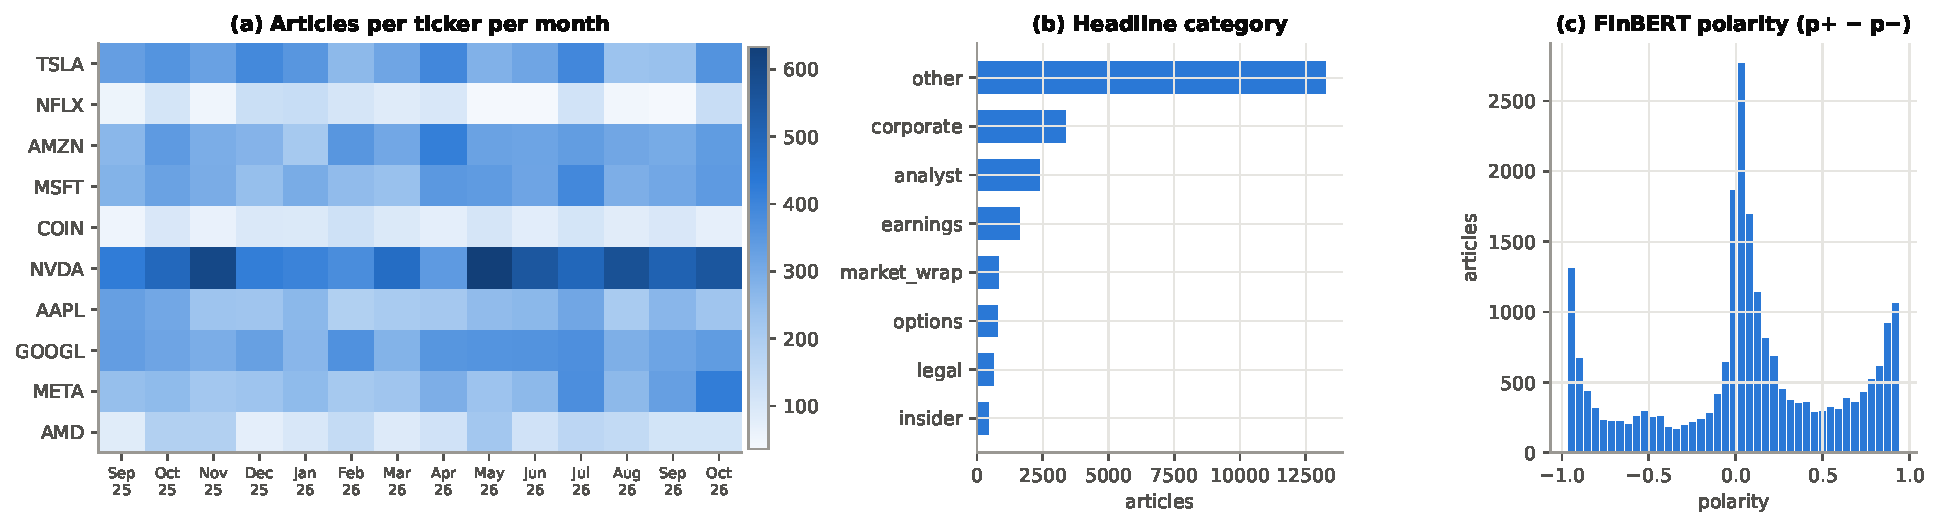
\includegraphics[width=\textwidth]{fig01_data_overview.pdf}
\caption{Dataset overview: (a) articles per ticker per month, (b) headline categories used by credibility learning, (c) distribution of FinBERT polarity.}
\label{fig:data}
\end{figure}

\subsection{Shared annotation}
Each headline receives a FinBERT polarity $s\in[-1,1]$ and each headline plus summary a unit-length MiniLM embedding $\mathbf{e}$. Headlines are also assigned a coarse category (analyst, earnings, options, insider, legal, market wrap, corporate, other) by keyword rules; this category is used only by N1. Every system receives exactly the same annotations.

\subsection{Baseline memories}
\label{sec:finmem-impl}
Both baselines use exactly the same data and annotations as our memory, so that every difference comes from the memory design.

\paragraph{Faithful FinMem.} We implement FinMem's scoring as described in Section~\ref{sec:finmem-bg}: recency $e^{-\delta/Q_l}$, relevancy $\mathbf{e}_E\cdot\mathbf{q}$ where $\mathbf{q}$ embeds the trading inquiry (``Can you make an investment decision on Tesla (TSLA) stock? \dots''), importance $\min(1,(v+b)\alpha_l^{\delta}/100)$ with $v$ drawn from FinMem's layer probabilities ($\{0.8,0.15,0.05\}$, $\{0.05,0.8,0.15\}$, $\{0.05,0.15,0.8\}$ over $\{40,60,80\}$) and $b$ the access-counter bonus. News enters the shallow layer, 10-Qs the intermediate and 10-Ks the deep layer. Shallow memories are purged when recency $<0.05$ or importance $<5$. After each outcome is known, the top-3 retrieved memories whose polarity sign matched the realised return receive $b \mathrel{+}= 5$; a memory whose $v+b$ reaches 60 (80) moves to the intermediate (deep) layer and its recency is reset. The top $K=5$ memories of each layer are retrieved. Deviations from the original are deliberate and apply equally to all systems: open encoders instead of GPT summaries and \texttt{ada-002} embeddings, and no purging in the intermediate and deep layers, which hold the filings (FinMem keeps a report for its reporting cycle) and promoted news.

\paragraph{Plain RAG baseline.} A single pool with recency $e^{-\delta/14}$ plus relevancy and the top 5 items overall, in the spirit of Generative Agents without importance or layers.

\subsection{Proposed self-correcting memory (N1--N7)}
Our memory (called ``Ours'' in tables and figures) keeps the layered core described above and adds seven components, each of which can be switched off for ablation. They follow the \emph{remember--verify--act} idea of Chapter~\ref{ch:intro} (Table~\ref{tab:rva}): N2, N4, N5 and N6 decide what is stored and retrieved, N1, N3 and N7 check whether a memory should be trusted or acted on, and the decision policies and guardrails turn the verified context into an action.
\begin{table}[H]
\centering
\caption{The seven components of our memory grouped by role.}
\label{tab:rva}
\small
\begin{tabular}{p{0.13\textwidth}p{0.34\textwidth}p{0.45\textwidth}}
\hline
Role & Component & What it fixes \\
\hline
Remember & N2 near-duplicate consolidation & the same story stored many times \\
 & N4 situational query & retrieval ignores what is happening today \\
 & N5 data-driven importance & importance drawn at random \\
 & N6 point-in-time peer graph & news about related companies ignored \\
\hline
Verify & N1 hierarchical source credibility & every source trusted equally \\
 & N3 contradiction retirement & contradicted facts kept until they decay \\
 & N7 outcome-aware episodic recall & no learning from the agent's own outcomes \\
\hline
Act & decision policies, guardrails & rule, ML and LLM decisions; budget limits and approvals in the application \\
\hline
\end{tabular}
\end{table}

\paragraph{N1 -- Hierarchical online source credibility.} For every visible article with $|s|\ge 0.2$, once its next-day outcome is known we record a hit if $\operatorname{sign}(s)=\operatorname{sign}(r_{t+1}-r^{\text{SPY}}_{t+1})$ (market-adjusted). Credibility is a Beta--Bernoulli posterior shrunk from author to category to global:
\begin{equation}
c_g=\frac{h_g+m\cdot 0.5}{n_g+m},\qquad c_k=\frac{h_k+m\,c_g}{n_k+m},\qquad c_a=\frac{h_a+m\,c_k}{n_a+m},
\end{equation}
with prior strength $m=8$, where $h$ and $n$ are hits and observations for the global pool $g$, the headline category $k$ and the author $a$. Credible memories gain $2(c-0.5)$ in retrieval score and enter the signal with weight $w=\operatorname{clip}(2(c-0.5),0,1)+0.05$. Updates use only resolved outcomes, so the estimate is point-in-time.

\paragraph{N2 -- Near-duplicate consolidation.} An incoming item whose embedding has cosine similarity $\ge 0.88$ with an active memory of the same layer and the same polarity sign does not create a new memory; instead the stored memory's corroboration count $n_c$ increases and its timestamp is refreshed. Corroboration adds $10\ln n_c$ importance points and multiplies the evidence weight by $1+\ln n_c$.

\paragraph{N3 -- Semantic contradiction retirement.} If a new item with $|s|\ge 0.3$ has similarity $\ge 0.72$ with an older active memory of the same layer whose polarity is opposite and $|s|\ge 0.3$, the older memory is retired.

\paragraph{N4 -- Situational query.} The query is $\mathbf{q}=\operatorname{normalize}(\mathbf{q}_{\text{task}}+\bar{\mathbf{e}}_{\text{today}})$, where $\bar{\mathbf{e}}_{\text{today}}$ is the mean embedding of the ticker's articles of the day, so that retrieval looks for memories related to what is happening now.

\paragraph{N5 -- Data-driven importance.} Instead of a random draw, $v = 40 + 40\cdot\operatorname{clip}\!\big(0.5|s|+0.5\tanh(a-1),0,1\big) + 20\,l$, where $a=(n_{\text{today}}+1)/(\bar n_{20}+1)$ is the news-attention surprise relative to the previous 20 sessions and $l\in\{0,1,2\}$ the layer index.

\paragraph{N6 -- Point-in-time peer graph.} Articles naming two to six symbols form a co-mention graph over a rolling 120-day window (only past days). The three most co-mentioned universe peers receive weights $w_p$ proportional to their counts; up to three same-day articles about each peer that do not mention the focal ticker, chosen by similarity to the query, contribute with weight $0.5\,w_p\,w(c)$.

\paragraph{N7 -- Outcome-aware episodic memory.} Every decision stores an episode: the context vector (weighted mean embedding of the retrieved memories), the signal $S$ and the realised market-adjusted return $\tilde r$. At decision time the ten most similar past contexts with similarity $>0.3$ are recalled; if at least five exist, the edge is
\begin{equation}
\epsilon=\frac{\sum_j \text{sim}_j\,\operatorname{sign}(S_j)\,\tilde r_j}{\sum_j \text{sim}_j},
\end{equation}
and the agent abstains (keeps its position) when $\epsilon<0$, i.e.\ when acting on the news signal in similar situations lost money.

\paragraph{Evidence aggregation.} For retrieved memories $i$ (and peer items) with polarity $s_i$ and weight $w_i$ ($w_i=1$ for the baselines), the memory signal is
\begin{equation}
S=\frac{\sum_i w_i s_i}{\sum_i |w_i|}\in[-1,1].
\end{equation}

\subsection{Decision policies}
\begin{itemize}
  \item \textbf{Threshold rule (all memories).} Buy if $S>\theta$, Sell if $S<-\theta$, otherwise Hold, with FinMem's semantics: Buy holds a long position, Sell a short position, Hold keeps the current position. $\theta\in\{0,0.05,0.1,0.15,0.2,0.3,0.4\}$ is chosen per system (Section~\ref{sec:protocols}).
  \item \textbf{Rule baselines.} Buy-and-hold; 1-day momentum; 20-day time-series momentum; 5-day mean reversion; 20-day moving-average crossover; and the sign of the day's average headline polarity (no memory).
  \item \textbf{Learned baselines.} Logistic regression and LightGBM~\cite{ke2017lightgbm} predicting the sign of the next-day return from nine price features (1/5/20-day returns, 20-day volatility, RSI, distance to the 20-day average, volume z-score, SPY 1/5-day returns), optionally with FinMem's or our memory features. Long when $P(\text{up})>0.5+\mu$, short when $<0.5-\mu$.
  \item \textbf{LLM backbones.} The retrieved memories (with credibility and corroboration tags and the peer and episodic summaries for ours), 3-day momentum, the current position and FinMem's self-adaptive character are rendered into a prompt; the model returns JSON with action, confidence, reasoning and cited memory IDs. We use three free models on Groq, \texttt{gpt-oss-120b}, \texttt{gpt-oss-20b} and \texttt{qwen3.8-27b}, with temperature 0 and no cross-model fallback. OpenRouter's free models were tried but dropped: on a free account all free models share a cap of 50 requests per day, and the one uncapped model we found was throttled upstream to about 30 requests per hour.
\end{itemize}

\subsection{Extension models}
\label{sec:ext-design}
To test whether the conclusions depend on the model family, we added five models that use the same (ticker, date) grid, the same test window, monthly walk-forward re-fitting, the same probability margin $\mu=0.02$ and the same 5\,bps costs as LightGBM. All settings were fixed before the first run.
\begin{itemize}
  \item \textbf{GRU (price).} For every (ticker, day), the nine price features of the last $L=20$ trading days are standardised with training-window statistics, clipped to $\pm5$ and fed to a one-layer GRU with 32 hidden units and a 4-dimensional ticker embedding; the last hidden state gives $P(\text{up})$ through a linear layer.
  \item \textbf{Transformer (price).} The same window is projected to $d=32$, a learned positional embedding and a ticker embedding are added, and two Transformer encoder layers (2 heads, feed-forward size 64, dropout 0.1) process it; the representation of the decision day predicts $P(\text{up})$ (Figure~\ref{fig:transformer-arch}).
  \item \textbf{Transformer (price+memory).} The same network with our memory features (signal, day sentiment, number of articles, conflict, redundancy, mean age, layer counts, peer signal, episodic edge, mean credibility) added to every day of the window.
  \item \textbf{Training.} Binary cross-entropy on the sign of the next-day return, AdamW~\cite{loshchilov2019adamw} (learning rate $10^{-3}$, weight decay $10^{-3}$), batch 64, gradient clipping 1.0, at most 40 epochs with early stopping (patience 6) on the last 15\% of the training rows in time order; three seeds are averaged, as for LightGBM. The model is refitted at the start of every test month on all labels that were resolved before the month began.
  \item \textbf{RL Q-learning.} A tabular agent (Section~\ref{sec:rl-bg}) with state $s=(\text{5-day move}\in\{\downarrow,\approx,\uparrow\}$ at $\pm2\%$, price above/below its 20-day average, RSI band $<35$/$35$--$65$/$>65$, current position$)$, i.e.\ 36 states, and actions Flat or Long. The reward is the next-day return of the chosen position minus 5\,bps per switch; $\alpha=0.1$, $\gamma=0.9$. It pre-trains for 30 passes on the history of all ten stocks before December 2025 with $\varepsilon$ decaying from 1 to 0.05, then trades the test window greedily. After each day's return becomes known it updates $Q$ from that day's experience of all ten stocks; because the market return does not depend on the agent, the rewards of both actions are known and both are learned from.
  \item \textbf{Pattern analogues (kNN).} For each stock and day, the 8 most similar past 20-day windows of the same stock (Pearson correlation of z-normalised log prices, non-overlapping, outcome fully observed) vote with similarity weights on the 10-day forward return; Buy if the expected move exceeds 1\% and $P(\text{up})\ge0.55$, Sell if it is below $-1\%$ and $P(\text{up})\le0.45$, otherwise Hold. These are the application's default settings, chosen before any test result.
  \item \textbf{Exploratory combinations} (defined \emph{after} the main results and reported separately): a \emph{risk overlay} that takes LightGBM's position but stays in cash whenever our memory abstains (N7), and a \emph{model vote} that takes the majority sign of LightGBM, the Transformer and our memory.
\end{itemize}

\begin{figure}[H]
\centering
\begin{tikzpicture}[every node/.style={font=\footnotesize},
  box/.style={rectangle, draw, rounded corners, thick, align=center, minimum height=0.8cm},
  arr/.style={-{Latex[length=1.8mm]}, thick}]
\node[box, fill=gray!10, minimum width=3.2cm] (in) at (0,0) {20 days $\times$ 9 price\\features (z-scored)};
\node[box, fill=blue!8, minimum width=3.0cm] (proj) at (4,0) {Linear $9\!\to\!32$\\+ position + ticker emb.};
\node[box, fill=violet!12, minimum width=3.0cm] (enc1) at (8,0) {Encoder layer 1\\2-head attention + FFN};
\node[box, fill=violet!12, minimum width=3.0cm] (enc2) at (8,-1.5) {Encoder layer 2\\2-head attention + FFN};
\node[box, fill=green!10, minimum width=3.0cm] (head) at (4,-1.5) {LayerNorm + Linear\\on decision day};
\node[box, fill=gray!10, minimum width=3.2cm] (out) at (0,-1.5) {$P(\text{up})\to$ long/short\\if $|P-0.5|>0.02$};
\draw[arr] (in) -- (proj); \draw[arr] (proj) -- (enc1); \draw[arr] (enc1) -- (enc2); \draw[arr] (enc2) -- (head); \draw[arr] (head) -- (out);
\end{tikzpicture}
\caption{Transformer model used as an extension baseline (refitted monthly, three seeds).}
\label{fig:transformer-arch}
\end{figure}

\subsection{Safe-autonomy design of the application}
\label{sec:autopilot-design}
The application lets the agent trade on its own, but because our results show that no signal is reliably predictive, autonomy is wrapped in layered controls (Figure~\ref{fig:autopilot-flow}).
\begin{enumerate}
  \item \textbf{Decision.} On a schedule (or on demand) the autopilot rotates through the allowed stocks and asks the chosen decision mode for Buy/Sell/Hold: the memory--price consensus, an LLM backbone, or both, where disagreement turns into Hold.
  \item \textbf{Hard guardrail.} One function, \texttt{gate}, sizes the order and applies the hard limits: emergency stop, allowed stocks, cash reserve, per-stock cap, single-order cap, daily-loss limit, drawdown limit from the equity peak and trades per day. A buy is sized as $\min(\text{target}-\text{held},\ \text{cash above reserve},\ \text{order cap})$; the agent never opens short positions; risk-reducing sells are only blocked by the emergency stop.
  \item \textbf{Permission mode.} \emph{Suggest only} logs what it would do; \emph{approval required} puts every trade in a queue (exits may optionally run at once); \emph{guarded automatic} executes small, confident, uncontested trades and queues the rest (confidence below a minimum, order above an automatic limit, or LLM--rule disagreement); \emph{fully automatic} executes everything that passes the hard limits.
  \item \textbf{Approval.} Queued proposals expire after 30 minutes and are re-checked against the hard limits at the moment of approval, never for more than the approved amount.
  \item \textbf{Audit.} Every decision, block, approval, rejection and expiry is written to an append-only log shown in the interface.
\end{enumerate}

\begin{figure}[H]
\centering
\begin{tikzpicture}[every node/.style={font=\footnotesize},
  box/.style={rectangle, draw, rounded corners, thick, align=center, minimum height=0.8cm, minimum width=2.6cm},
  dec/.style={diamond, draw, thick, aspect=2.2, align=center, inner sep=1pt},
  arr/.style={-{Latex[length=1.8mm]}, thick}]
\node[box, fill=gray!10] (sched) at (0,0) {Scheduler / user\\(market hours)};
\node[box, fill=blue!8] (dec) at (3.4,0) {Decision mode\\rules | LLM | both};
\node[dec, fill=orange!10] (gate) at (7.2,0) {Hard\\guardrail};
\node[box, fill=red!8] (block) at (7.2,-1.9) {Blocked / skipped\\(logged)};
\node[dec, fill=violet!10] (mode) at (11,0) {Permission\\mode};
\node[box, fill=green!10] (exec) at (11,-1.9) {Execute on\\paper account};
\node[box, fill=yellow!15] (queue) at (11,1.9) {Approval queue\\(30 min)};
\node[box, fill=gray!10] (sugg) at (7.2,1.9) {Suggestion only\\(logged)};
\draw[arr] (sched) -- (dec); \draw[arr] (dec) -- (gate);
\draw[arr] (gate) -- node[right]{fails} (block);
\draw[arr] (gate) -- node[above]{passes} (mode);
\draw[arr] (mode) -- node[right]{full / guarded, no flag} (exec);
\draw[arr] (mode) -- node[right]{approve / guarded, flagged} (queue);
\draw[arr] (mode.north west) -- node[above left]{suggest} (sugg);
\draw[arr] (queue.east) to[out=-30,in=30] node[right]{approved + re-checked} (exec.east);
\end{tikzpicture}
\caption{Every order of the autopilot passes one hard guardrail and then the user's permission mode.}
\label{fig:autopilot-flow}
\end{figure}

\paragraph{Budget allocation.} For a budget $B$, cash reserve $c$ and per-stock cap $m$, the investable share is $1-c$ and each weight is capped at $m/(1-c)$ of it, with the excess redistributed proportionally. Inverse-volatility weights are $w_i\propto1/\sigma_i$, minimum-variance weights solve $\min_w w^\top\Sigma w$ s.t.\ $\sum w_i=1$, $0\le w_i\le m/(1-c)$ (SLSQP), and the signal-tilted variant multiplies inverse-volatility weights by 1.5, 1 or 0 for today's Buy, Hold or Sell consensus. The methods are compared walk-forward: every 21 trading days the weights are recomputed from the previous 120 days only.

\paragraph{Credential handling.} Keys pasted in the interface are first tested with one authenticated call to the provider (account status for Alpaca, the model list for Groq, the key endpoint for OpenRouter); only valid keys are stored in a git-ignored file with owner-only permissions and are applied to the process environment immediately, so no restart is needed. The browser only receives masked keys. Write and read requests are accepted only from the local machine and from the application's own origin, which blocks malicious web pages and DNS-rebinding attempts.

\subsection{Evaluation protocols}
\label{sec:protocols}
\begin{itemize}
  \item \textbf{Rolling walk-forward (primary).} Memories are warmed up in September 2025. From December 2025 to October 2026 (227 sessions), at the start of each month the threshold $\theta$ of every system is chosen to maximise the Sharpe ratio over the previous 42 sessions, and the ML models are re-fitted on all earlier data (margin $\mu=0.02$ fixed in advance).
  \item \textbf{Fixed split (secondary).} Train October 2025 -- February 2026, validation March--April 2026 ($\theta$ and $\mu$ selection), test May--October 2026 (123 sessions).
\end{itemize}
Portfolios are equal-weight across tickers, net of 5\,bps. Ours is compared with every baseline by a paired Wilcoxon test on pooled (ticker, date) returns with Holm correction, a paired $t$-test, a Diebold--Mariano test and a 10-day moving-block bootstrap (5{,}000 resamples) of the Sharpe difference of the portfolios. The predictive content of each memory signal is measured by its Spearman IC with the next-day market-adjusted return.

\subsection{Alternatives considered}
\begin{itemize}
  \item \textbf{LLM-based sentiment and summaries} (as in FinMem) would cost thousands of calls on rate-limited free tiers and make annotations non-deterministic; FinBERT and MiniLM are free, fast and reproducible.
  \item \textbf{A vector database} (FAISS) is unnecessary at our scale (at most a few thousand active memories per ticker); an in-memory NumPy store keeps the code simple and testable.
  \item \textbf{Deep reinforcement learning baselines} (PPO, DQN, A2C) need years of training data and are sensitive to seeds; instead we use a tabular Q-learning agent whose 36 states can be inspected one by one, alongside compact GRU and Transformer models that can be refitted monthly on a CPU.
  \item \textbf{Large pre-trained time-series Transformers} would add parameters that one year of daily data cannot constrain; we keep the Transformer small (about 20k parameters) and average three seeds.
  \item \textbf{A single test window} (FinMem's protocol) is simpler but fragile; we report it only as a secondary protocol.
  \item \textbf{Signed credibility}, which lets contrarian sources vote in the opposite direction, was tried after the first fixed-split run; because this was a post-hoc choice it is reported separately and not used in the main model.
\end{itemize}

\section{Project Plan}
The project ran over three trimesters (Table~\ref{tab:plan}).
\begin{table}[H]
\centering
\caption{Project schedule.}
\label{tab:plan}
\begin{tabular}{llp{0.62\textwidth}}
\hline
Trimester & Phase & Activities \\
\hline
Fall 2025 & 1 & Literature review, analysis of FinMem, problem definition and project proposal \\
Spring 2026 & 2 & Requirements, system design, data pipeline, prototype memory, dashboard and paper-trading adapter \\
Summer 2026 & 3 & One-year dataset, faithful FinMem, proposed memory N1--N7, experiments, ablations, LLM backbones and extension models \\
 & 4 & Application integration (autopilot, analytics, Bangla interface), testing, report and presentation \\
\hline
\end{tabular}
\end{table}

\section{Task Allocation}
All members took part in the analysis of the FinMem paper, the project proposal, the report and the presentations; the main responsibility of each member is listed in Table~\ref{tab:tasks}.
\begin{table}[H]
\centering
\caption{Task allocation.}
\label{tab:tasks}
\small
\begin{tabular}{p{0.27\textwidth}p{0.14\textwidth}p{0.5\textwidth}}
\hline
Member & ID & Main responsibility \\
\hline
Md. Nurul Huda & 0112230303 & System design and implementation: faithful FinMem, memory components N1--N7, extension models, statistical evaluation and the application \\
Atkia Fayrose Prity & 0112230101 & Literature review (FinMem and related LLM-agent, memory and back-testing work), background and gap analysis; design of the plain-language explanations and Bangla interface text \\
Tanjila Tafrim Priyonta & 0112230111 & Results analysis (tables, figures, significance and robustness findings, limitations); usability testing of the application in both languages, themes and on mobile \\
Ankita Saha & 0112310509 & Data pipeline: news, SEC filing and price collection, point-in-time alignment and annotation; report structure in the UIU template, references, standards and design constraints \\
MD. Mahmud Hasan & 0112230995 & Experiments and testing: running the study, ablation and LLM-backbone experiments, automated tests; project proposal, slides and application demonstration \\
\hline
\end{tabular}
\end{table}

\section{Summary}
We specified functional and non-functional requirements, described the system's context, data flow and interface, and detailed the methodology: point-in-time data, the baseline memories, our self-correcting memory with its seven remember-and-verify components, the decision policies, the extension models (GRU, Transformer, Q-learning, pattern analogues), the safe-autonomy design of the application and two evaluation protocols with appropriate statistics.

\chapter{Implementation and Results}
\label{ch:impl}

This chapter describes the software environment and implementation, how the system was tested, and the experimental results: overall performance under both protocols, statistical tests, per-ticker and FinMem-universe results, predictive content, ablations, sensitivity analyses, retrieval diagnostics, the LLM-backbone comparison, the extension models (GRU, Transformer, reinforcement learning, pattern analogues), portfolio construction, robustness and power analyses, and the evaluation of the application.

\section{Environment Setup}
\begin{itemize}
  \item \textbf{Hardware}: a laptop with an 8-core CPU and 8\,GB RAM; no GPU is required (FinBERT and MiniLM run on CPU; annotating 23{,}247 articles took about 50 minutes, a full replay of 16 memory configurations about 15 minutes).
  \item \textbf{Software}: Python 3.13, pandas, NumPy, SciPy, scikit-learn, LightGBM, PyTorch (CPU), Hugging Face Transformers and Sentence-Transformers, Matplotlib; the web server uses only the Python standard library and the front end is plain HTML, CSS and JavaScript with hand-written SVG charts.
  \item \textbf{External services}: Alpaca Market Data (news and SIP bars) and Alpaca paper trading, SEC EDGAR XBRL API, Groq and OpenRouter free tiers. Credentials are read from a local \texttt{.env} file that is excluded from version control.
  \item \textbf{Code organisation} (\texttt{src/agentic\_trade/study}): \texttt{data.py} (download, alignment, incremental refresh), \texttt{annotate.py}, \texttt{memory.py} (all memories and N1--N7 flags), \texttt{backtest.py} (day-major replay), \texttt{policies.py}, \texttt{evaluation.py}, \texttt{pipeline.py} (protocols), \texttt{llm\_agent.py}, \texttt{figures.py}; the extension experiments are in \texttt{study/extensions.py}. The application consists of \texttt{dashboard\_server.py} (HTTP API), \texttt{agent\_service.py} (research agent), \texttt{autopilot.py} (budget, guardrails, permission modes, scheduler), \texttt{analytics.py} (pattern analogues, risk, correlation, allocation, Monte Carlo), \texttt{algorithms.py} (algorithm board and Q-learning agent) and \texttt{credentials.py} (API-key management), and a front end split into \texttt{core.js} (navigation, global stock, language, theme), \texttt{i18n.js} (about 750 English/Bangla strings), \texttt{charts.js}, \texttt{trade.js}, \texttt{autopilot.js}, \texttt{analytics.js}, \texttt{app.js} and \texttt{credentials.js}. Scripts \texttt{build\_dataset.py}, \texttt{run\_study.py}, \texttt{run\_llm\_study.py}, \texttt{run\_extensions.py}, \texttt{make\_extension\_figures.py}, \texttt{export\_latex\_tables.py}, \texttt{export\_extension\_tables.py} and \texttt{capture\_app\_screens.py} reproduce the dataset, results, figures, tables and screenshots in this report.
\end{itemize}

The replay is \emph{day-major}: all tickers advance together, so information shared across tickers (source credibility) can only contain outcomes that were already public. Each memory keeps its items in pre-allocated NumPy arrays, so a retrieval is a masked matrix--vector product followed by a per-layer partial sort.

\section{Testing and Evaluation}
The repository contains \testcount{} automated tests (pytest), all passing. The study-specific tests check:
\begin{itemize}
  \item point-in-time alignment (an article at 15:59 New York time belongs to the same session, at 16:01 to the next; weekend news to Monday);
  \item that retrieval never returns future items and that FinMem retrieves per layer;
  \item FinMem's decay constants, purge rule and access-counter promotion with recency reset;
  \item that duplicates are merged and contradictions retired only in our memory, never in FinMem;
  \item credibility shrinkage (an unseen author inherits the category estimate);
  \item episodic recall requiring at least five similar episodes;
  \item Hold-keeps-position semantics and transaction-cost accounting;
  \item non-overlapping splits, metric and Holm-correction helpers;
  \item the application's consensus rule (agreement, disagreement, abstention, weak price signals) and that the agent brief is built from the research memory.
\end{itemize}
Tests added for the extensions and the application check:
\begin{itemize}
  \item the Q-learning agent cannot look ahead: changing the last five days of prices leaves every earlier decision and the learning curve unchanged, and it is deterministic for a fixed seed;
  \item pattern analogues only use windows whose outcome was already known and never overlap the window being matched; an always-long analogue strategy reproduces buy-and-hold exactly;
  \item the guardrail sizes buys by the tightest of target, cash above reserve and order cap; blocks buys (but not exits) after the daily-loss or drawdown limit; enforces allowed stocks and trades per day; and the emergency stop cancels the queue and prevents re-enabling;
  \item every permission mode routes decisions as specified, approvals are re-checked and proposals expire;
  \item budget-split plans respect the reserve and the per-stock cap for every method, and their rebalancing amounts are consistent with current holdings;
  \item API keys are validated before saving, stored with owner-only permissions, never returned unmasked, and the endpoints refuse cross-origin and foreign-host requests;
  \item the experience log of the algorithm board is internally consistent (a long position is ``right'' exactly when the next-day return is positive).
\end{itemize}
Legacy tests cover the paper-trading adapter, risk limits, LLM output parsing and the dashboard APIs. Every view of the application was also exercised end to end in a headless browser in both languages and both themes, on desktop and phone widths, with the browser console checked for errors. The front-end dictionary is checked automatically: every key used in the HTML or JavaScript exists in both languages and every placeholder appears in both translations.

\section{Results and Discussion}

\subsection{Overall performance}
Table~\ref{tab:main} reports the primary rolling protocol and Figure~\ref{fig:equity} the equity curves. Among the three memory architectures, ours has the highest Sharpe ratio, the smallest loss and the smallest drawdown; FinMem and flat retrieval behave almost identically. However, all three news-memory policies lose money over the period, while buy-and-hold and, above all, the price-only LightGBM earn positive returns. Adding memory features to LightGBM \emph{reduces} its Sharpe ratio, indicating that the memory features mostly add noise for a tree model fitted on a few thousand observations.

\begin{table}[ht]
\centering
\caption{Ten-stock equal-weight portfolio, rolling walk-forward protocol (2025-12-01 to 2026-10-26, 227 sessions), net of 5\,bps. Best value per column in bold.}
\label{tab:main}
\small
\begin{tabular}{lrrrrrrr}
\hline
Strategy & CR (\%) & Sharpe & Sortino & Ann. Vol (\%) & MDD (\%) & Win (\%) & Turnover \\
\hline
Buy \& Hold & 11.15 & 0.61 & 0.96 & 23.82 & -16.50 & 50.2 & 0.00 \\
Momentum (1d) & -10.12 & -0.59 & -0.92 & 17.58 & -18.98 & 51.5 & 0.56 \\
TS-Momentum (20d) & -16.17 & -0.91 & -1.25 & 19.44 & -26.85 & 50.2 & 0.15 \\
Mean-Reversion (5d) & -4.54 & -0.21 & -0.30 & 17.22 & -21.57 & 48.0 & 0.30 \\
MA-Crossover & -3.37 & -0.12 & -0.16 & 18.02 & -19.62 & 53.3 & 0.17 \\
Daily News Sentiment & -22.24 & -2.26 & -3.11 & 12.05 & -23.32 & 42.7 & 0.38 \\ \hline
LogReg (price) & -21.54 & -1.39 & -2.13 & 18.20 & -29.66 & 47.1 & 0.20 \\
LGBM (price) & \textbf{19.40} & \textbf{1.15} & \textbf{1.91} & 18.59 & -17.15 & 54.2 & 0.70 \\
LGBM (price+FinMem) & 5.63 & 0.42 & 0.68 & 18.27 & -13.05 & 52.4 & 0.66 \\
LGBM (price+Ours) & 6.16 & 0.44 & 0.71 & 19.01 & \textbf{-11.03} & 51.1 & 0.60 \\ \hline
Plain RAG & -9.45 & -0.65 & -0.97 & 15.13 & -21.14 & 49.3 & 0.16 \\
FinMem & -10.98 & -0.72 & -1.03 & 16.11 & -19.69 & 48.5 & 0.07 \\
Ours & -3.56 & -0.20 & -0.30 & 14.84 & -15.18 & 49.3 & 0.06 \\
\hline
\end{tabular}
\end{table}


\begin{figure}[H]
\centering
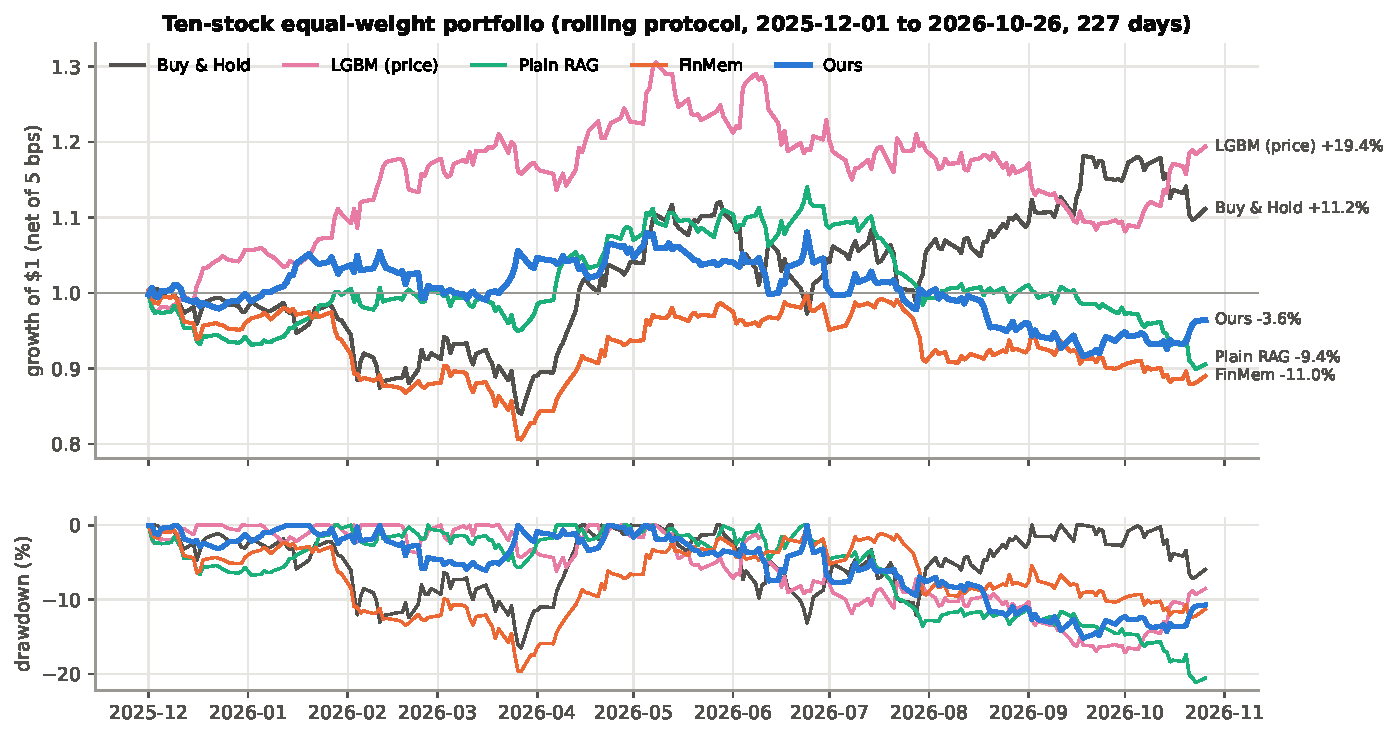
\includegraphics[width=\textwidth]{fig03_equity_portfolio.pdf}
\caption{Equal-weight ten-stock portfolio under the rolling protocol, net of costs, with drawdowns.}
\label{fig:equity}
\end{figure}

Two properties explain much of the gap to buy-and-hold. First, our memory abstains (keeps its position instead of acting on the signal) on 49\% of ticker-days because the episodic memory reports that similar situations were mis-signalled. Second, because Hold keeps the previous position, the memory policies are always invested, and ours is short on 58\% of ticker-days (FinMem 29\%, Plain RAG 43\%) in a market that rose over the period: its portfolio beta is $-0.33$ against $+0.64$ for FinMem (Figure~\ref{fig:positions}).

\begin{figure}[H]
\centering
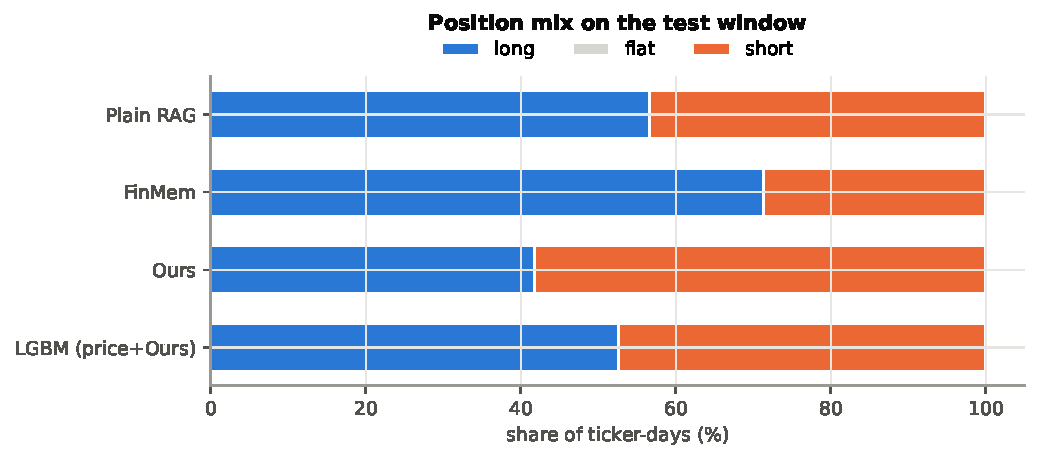
\includegraphics[width=0.75\textwidth]{fig17_positions.pdf}
\caption{Share of long, flat and short ticker-days in the test period.}
\label{fig:positions}
\end{figure}

\subsection{Statistical significance}
Table~\ref{tab:tests} compares ours with every baseline. Ours earns 3.4 basis points per day more than FinMem and has a Sharpe ratio higher by about 0.5, but the 95\% bootstrap interval of the difference contains zero and the Wilcoxon test is far from significance ($p=0.39$). The only Holm-significant differences are against the 1-day momentum rule and against trading on the day's headline tone without memory, i.e.\ memory is significantly better than reacting to today's news alone. Figure~\ref{fig:bootstrap} shows the bootstrap distributions.

\begin{table}[ht]
\centering
\caption{Ours versus every baseline on pooled (ticker, date) daily returns, rolling protocol. $\Delta$ = Ours $-$ baseline; CI from a 10-day moving-block bootstrap (5{,}000 resamples); Holm-adjusted Wilcoxon $p$; DM = Diebold--Mariano.}
\label{tab:tests}
\small
\begin{tabular}{lrrcrrr}
\hline
Baseline & $\Delta$ bps/day & $\Delta$Sharpe & 95\% CI & Wilcoxon $p$ & Holm $p$ & DM $p$ \\
\hline
Momentum (1d) & +2.9 & +0.39 & [-2.44, 2.85] & 0.000 & 0.000 & 0.723 \\
Daily News Sentiment & +9.6 & +2.06 & [-0.51, 4.38] & 0.000 & 0.001 & 0.164 \\
LGBM (price+FinMem) & -4.2 & -0.62 & [-3.34, 1.79] & 0.015 & 0.154 & 0.626 \\
LGBM (price) & -9.7 & -1.35 & [-3.99, 1.05] & 0.061 & 0.545 & 0.272 \\
LGBM (price+Ours) & -4.5 & -0.64 & [-2.92, 1.27] & 0.070 & 0.561 & 0.585 \\
LogReg (price) & +8.9 & +1.19 & [-1.18, 3.88] & 0.112 & 0.787 & 0.300 \\
TS-Momentum (20d) & +5.9 & +0.71 & [-1.68, 2.92] & 0.160 & 0.963 & 0.430 \\
Mean-Reversion (5d) & +0.3 & +0.02 & [-3.19, 2.67] & 0.308 & 1.000 & 0.973 \\
FinMem & +3.4 & +0.52 & [-2.73, 3.12] & 0.388 & 1.000 & 0.643 \\
MA-Crossover & -0.3 & -0.08 & [-2.16, 1.79] & 0.421 & 1.000 & 0.968 \\
Plain RAG & +2.8 & +0.46 & [-2.35, 2.36] & 0.426 & 1.000 & 0.683 \\
Buy \& Hold & -6.9 & -0.81 & [-4.11, 1.76] & 0.774 & 1.000 & 0.452 \\
\hline
\end{tabular}
\end{table}


\begin{figure}[H]
\centering
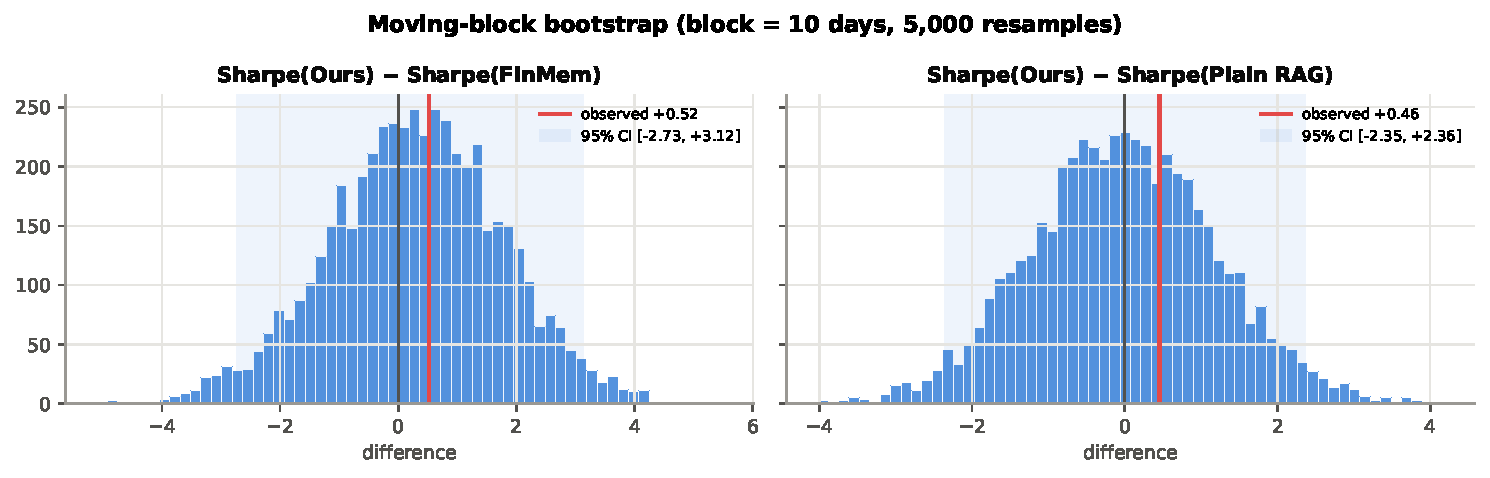
\includegraphics[width=\textwidth]{fig15_bootstrap.pdf}
\caption{Moving-block bootstrap distribution of the Sharpe difference between ours and FinMem (left) and Plain RAG (right).}
\label{fig:bootstrap}
\end{figure}

\subsection{FinMem's own stocks and per-ticker results}
On the five stocks FinMem was designed and evaluated on (Table~\ref{tab:finmem5}, Figure~\ref{fig:finmem5}), the difference is larger: FinMem and Plain RAG lose about 29\% while ours gains 3.5\%, also beating buy-and-hold ($-11.6\%$). Per ticker (Table~\ref{tab:perticker}, Figure~\ref{fig:heatmap}) the picture is mixed: ours is the best memory on NFLX, MSFT and COIN, but worse than FinMem on AMD, META, NVDA and TSLA. Such dispersion is expected when the underlying signal is weak.

\begin{table}[ht]
\centering
\caption{Equal-weight portfolio of FinMem's five stocks (TSLA, NFLX, AMZN, MSFT, COIN), rolling protocol, net of 5\,bps.}
\label{tab:finmem5}
\begin{tabular}{lrrrr}
\hline
System & CR (\%) & Sharpe & MDD (\%) & Ann. Vol (\%) \\
\hline
Buy \& Hold & -11.58 & -0.34 & -24.10 & 28.23 \\
Plain RAG & -28.82 & -1.59 & -31.61 & 22.20 \\
FinMem & -28.62 & -1.59 & -29.01 & 22.03 \\
Ours & \textbf{3.52} & \textbf{0.28} & \textbf{-20.03} & 22.35 \\
\hline
\end{tabular}
\end{table}


\begin{figure}[H]
\centering
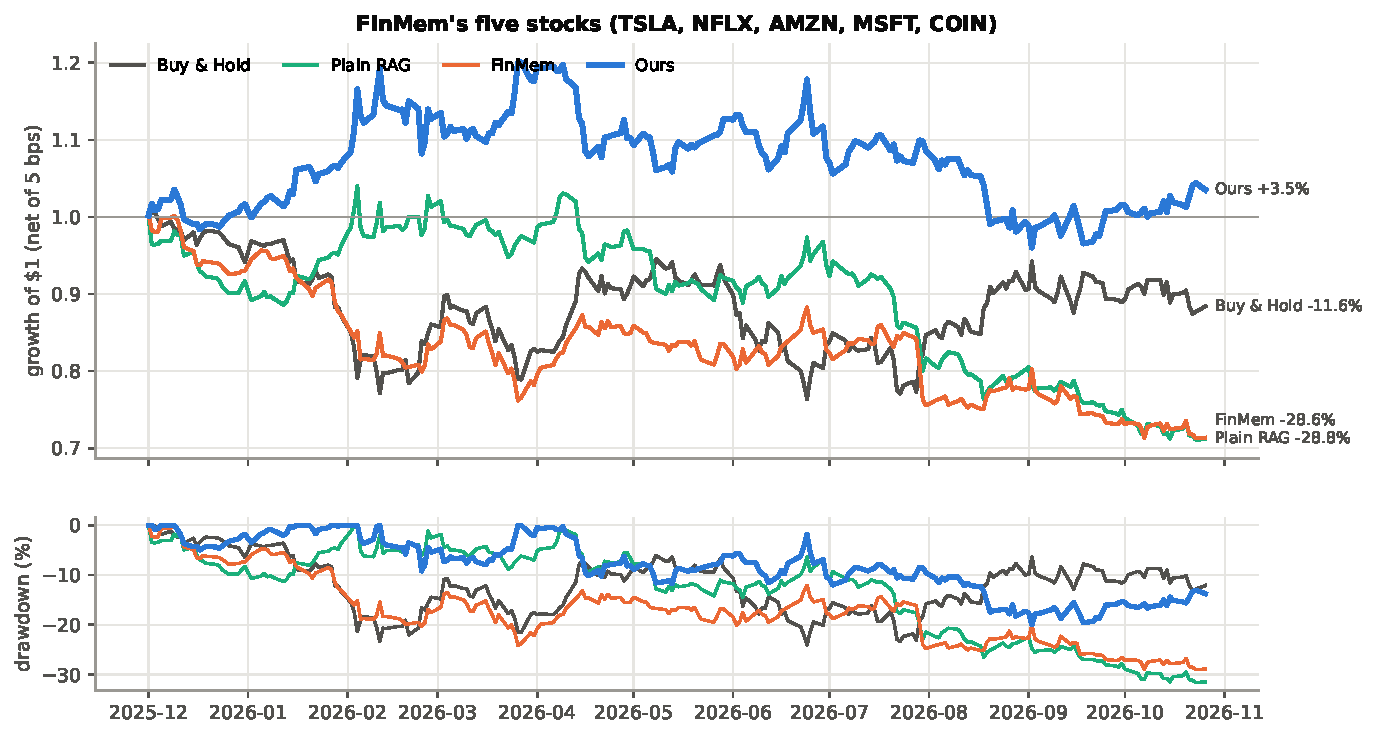
\includegraphics[width=\textwidth]{fig04_equity_finmem5.pdf}
\caption{Portfolio of FinMem's five stocks under the rolling protocol.}
\label{fig:finmem5}
\end{figure}

\begin{table}[ht]
\centering
\caption{Per-ticker Sharpe ratio, rolling protocol (net of costs).}
\label{tab:perticker}
\small
\setlength{\tabcolsep}{4pt}
\begin{tabular}{lrrrrrrrrrr}
\hline
Strategy & AAPL & AMD & AMZN & COIN & GOOGL & META & MSFT & NFLX & NVDA & TSLA \\
\hline
Buy \& Hold & 1.05 & 1.86 & 0.42 & -0.38 & 0.23 & 0.13 & 0.47 & -1.52 & 0.77 & 0.09 \\
LGBM (price) & -0.92 & 0.63 & 0.69 & 0.68 & 0.57 & 0.18 & -1.22 & -0.06 & 2.13 & 1.38 \\
Plain RAG & 0.75 & 0.26 & -0.76 & -1.55 & 1.86 & -0.40 & 0.31 & 0.94 & 0.03 & -1.90 \\
FinMem & 0.56 & 0.86 & -0.54 & -1.73 & -1.61 & 0.09 & 0.05 & 0.26 & 0.84 & -0.99 \\
Ours & 0.66 & 0.12 & -0.52 & 0.08 & 0.27 & -1.66 & 0.64 & 2.33 & -0.64 & -1.39 \\
\hline
\end{tabular}
\end{table}


\begin{figure}[H]
\centering
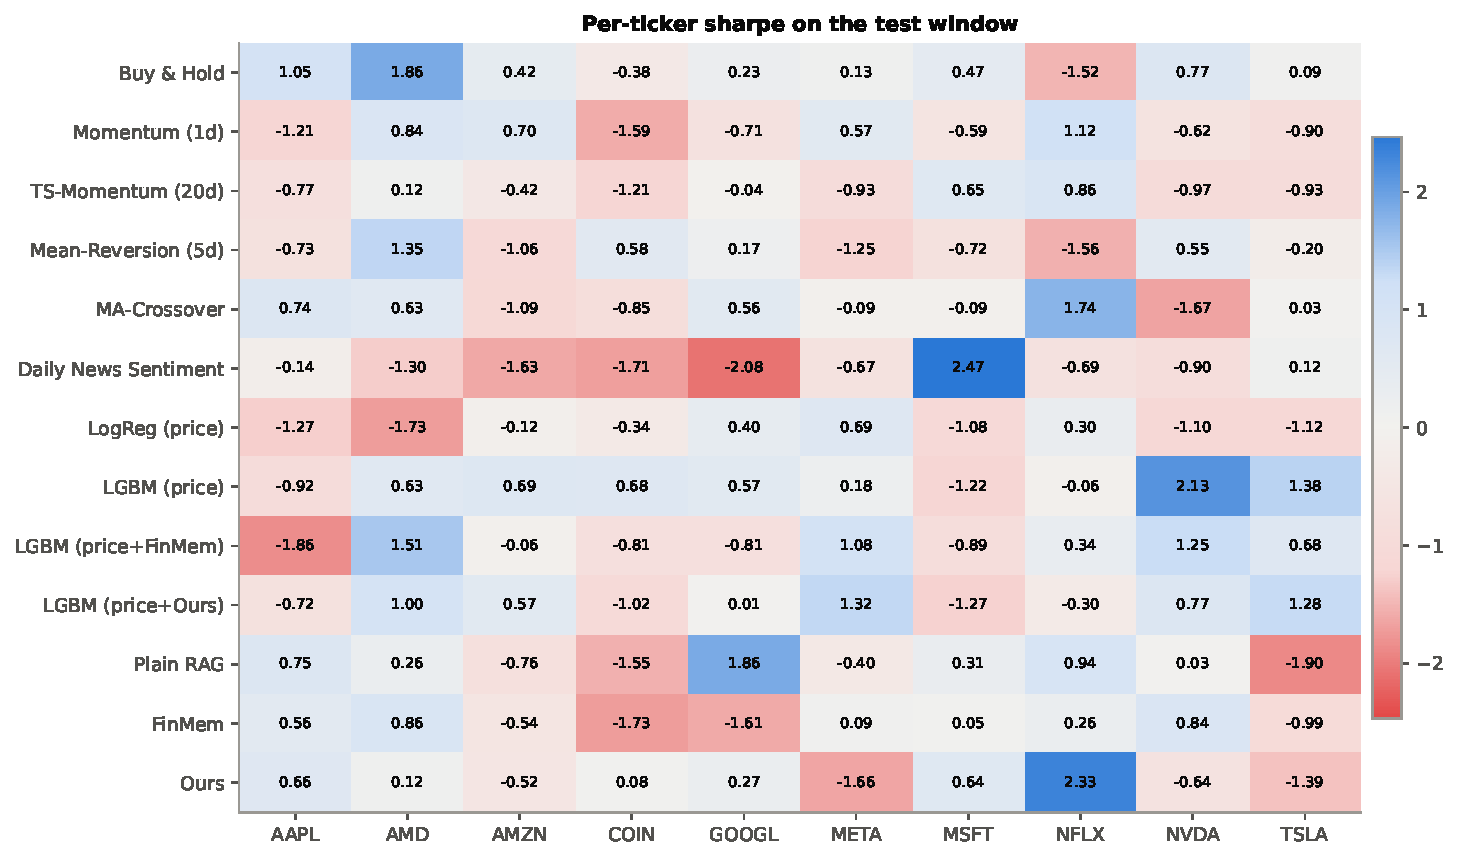
\includegraphics[width=\textwidth]{fig06_heatmap_sharpe.pdf}
\caption{Per-ticker Sharpe ratio of all strategies.}
\label{fig:heatmap}
\end{figure}

\begin{figure}[H]
\centering
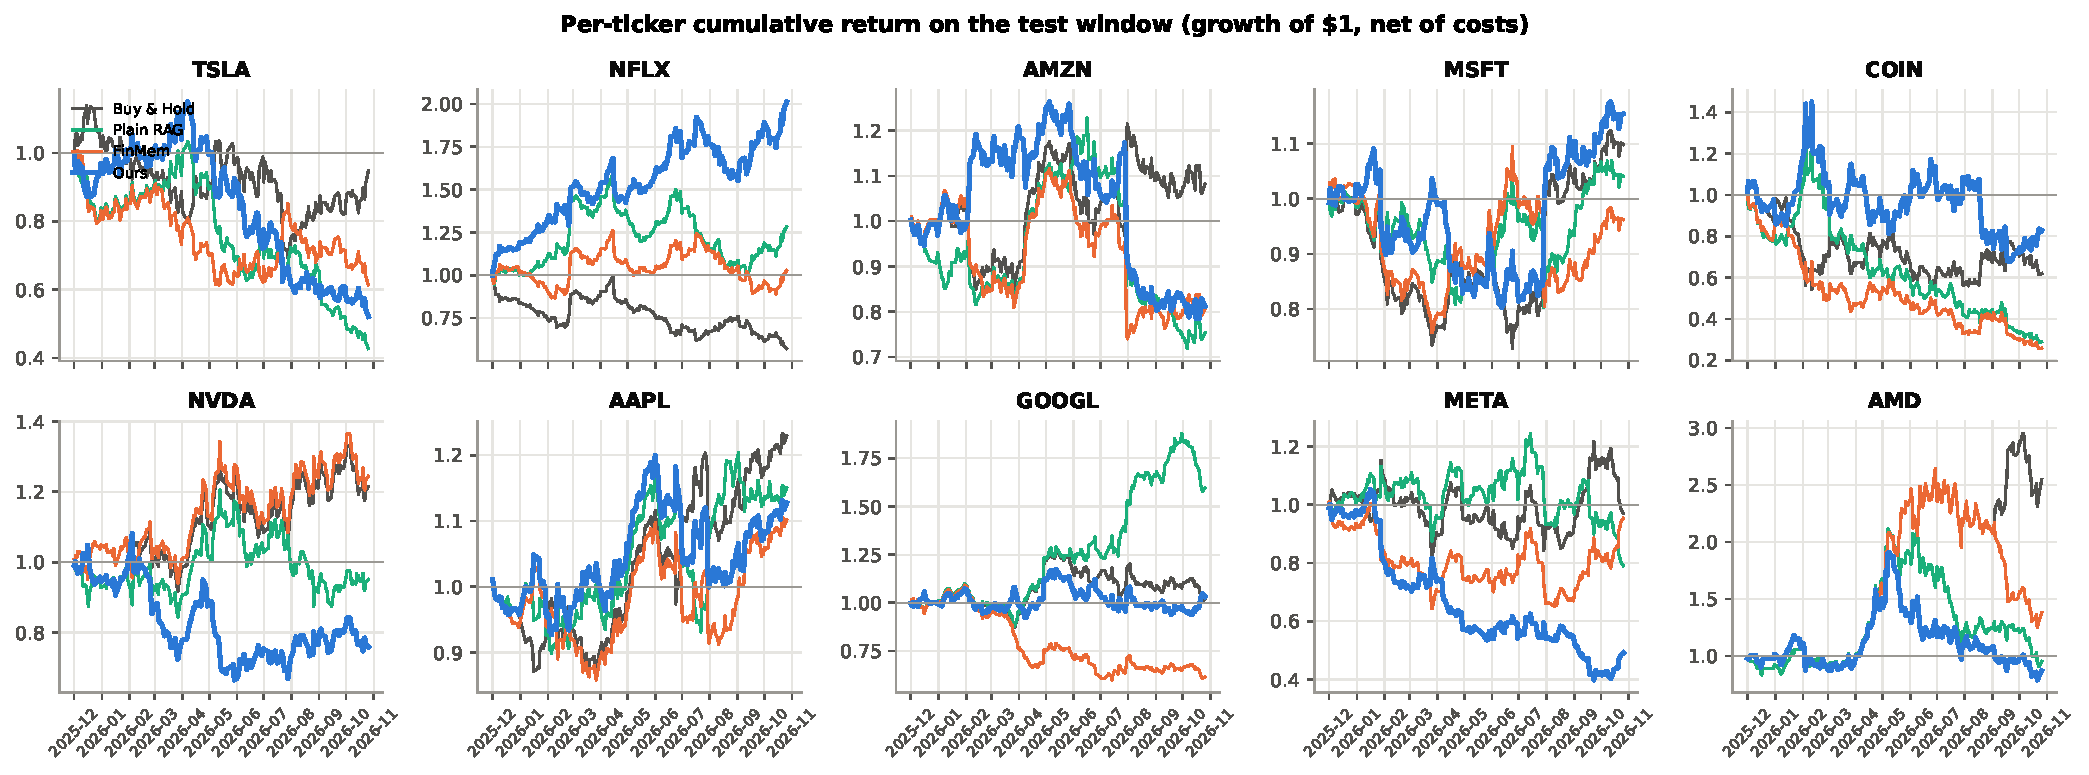
\includegraphics[width=\textwidth]{fig05_per_ticker.pdf}
\caption{Per-ticker cumulative returns of buy-and-hold and the three memories.}
\label{fig:perticker}
\end{figure}

\subsection{Predictive content of the memory}
Table~\ref{tab:icops} shows the Spearman IC between each memory signal and the next-day market-adjusted return. All values are within $\pm 0.04$ and none is significant at 5\%; flat retrieval of the most recent headlines is, if anything, slightly contrarian ($-0.037$, $p=0.08$), consistent with short-term reversal after news~\cite{chan2003stock,jegadeesh1990evidence}. This is the central empirical finding of the re-evaluation: in 2025--26, for these liquid large caps, the polarity of the retrieved news carries almost no information about the next day's move once it is public at the close, and FinMem's premise that better-organised news memory yields better daily trades does not hold on this data. The rolling 40-day Sharpe ratio (Figure~\ref{fig:rolling}) and monthly returns (Figure~\ref{fig:monthly}) confirm that relative performance changes sign across regimes.

\begin{table}[ht]
\centering
\caption{Predictive content of each memory signal (Spearman IC vs.\ next-day market-adjusted return, rolling test period) and memory operations over the full run (ten tickers).}
\label{tab:icops}
\small
\begin{tabular}{lrrrrrrrr}
\hline
System & IC & $p$ & IC (cross-sect.) & Items & Merged & Retired & Promoted & Purged \\
\hline
Plain RAG & -0.037 & 0.08 & -0.040 & 36,177 & 0 & 0 & 0 & 0 \\
FinMem & -0.000 & 0.99 & -0.007 & 36,177 & 0 & 0 & 1,221 & 32,625 \\
Ours & +0.003 & 0.90 & +0.015 & 33,917 & 2,260 & 667 & 1,510 & 29,417 \\
\hline
\end{tabular}
\end{table}


\begin{figure}[H]
\centering
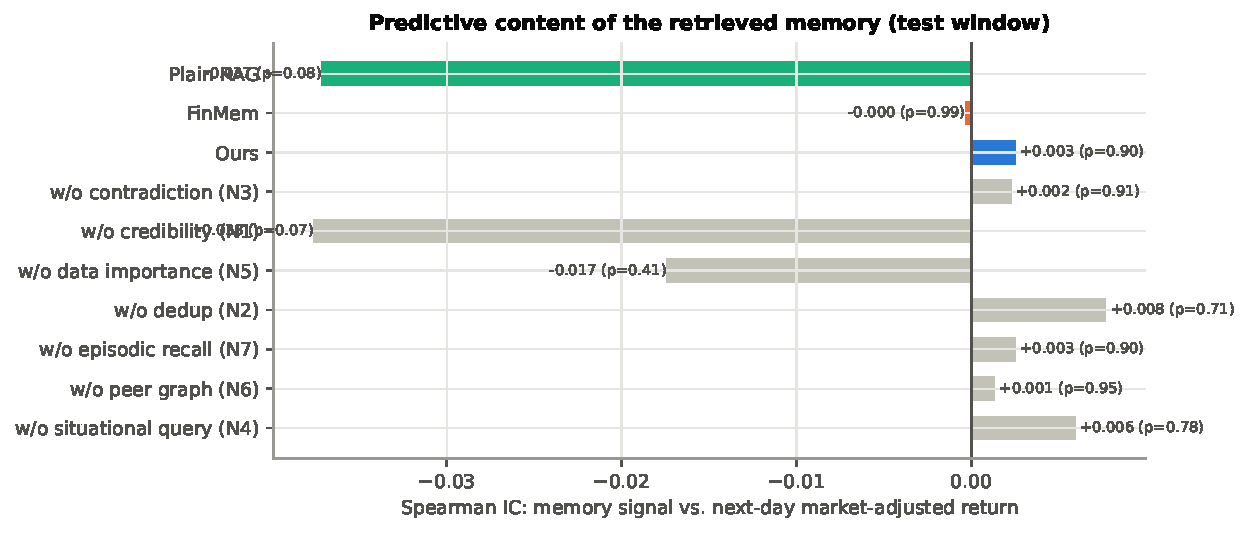
\includegraphics[width=0.85\textwidth]{fig12_information_coefficient.pdf}
\caption{Information coefficient of the memory signals, including ablated variants.}
\label{fig:ic}
\end{figure}

\begin{figure}[H]
\centering
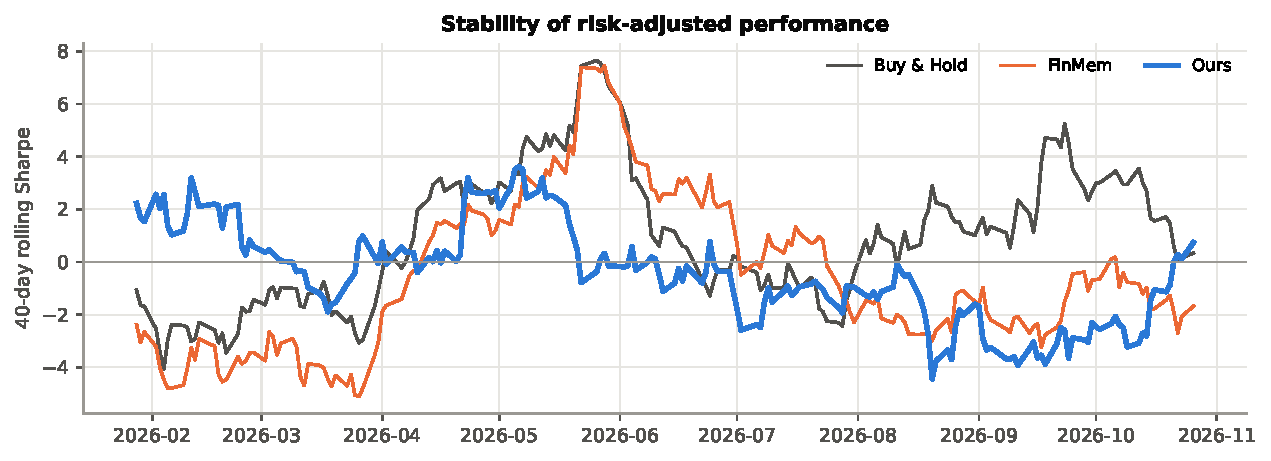
\includegraphics[width=\textwidth]{fig11_rolling_sharpe.pdf}
\caption{40-day rolling Sharpe ratio.}
\label{fig:rolling}
\end{figure}

\begin{figure}[H]
\centering
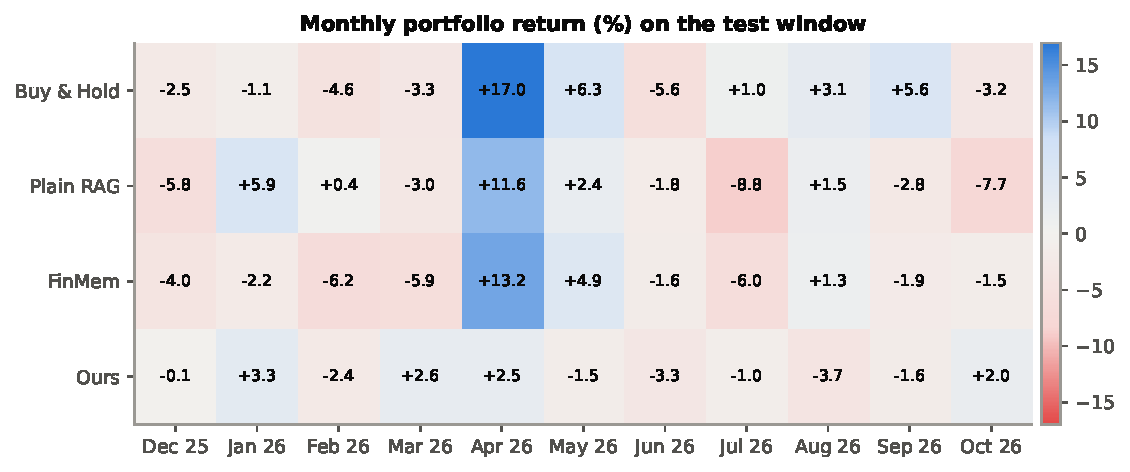
\includegraphics[width=0.85\textwidth]{fig16_monthly.pdf}
\caption{Monthly portfolio returns.}
\label{fig:monthly}
\end{figure}

\subsection{Ablation study}
Table~\ref{tab:ablation} and Figure~\ref{fig:ablation} remove one component at a time. The situational query (N4), the peer graph (N6) and data-driven importance (N5) contribute most to the Sharpe ratio. Removing episodic recall (N7) slightly increases the Sharpe ratio but raises the maximum drawdown from $-15.2\%$ to $-25.1\%$, and removing credibility (N1) raises it to $-18.6\%$: these two components act mainly as risk controls. Removing duplicate consolidation (N2) or contradiction retirement (N3) \emph{improves} the threshold policy; their benefit is in the quality and diversity of the context rather than in the aggregated polarity, which matters for an LLM reader but not for a polarity average. Given the noise level, differences of a few tenths of a Sharpe point should not be over-interpreted.

\begin{table}[ht]
\centering
\caption{Component ablation of our memory (rolling protocol). Each row removes one component; ``FinMem'' removes all of them.}
\label{tab:ablation}
\begin{tabular}{lrrrrr}
\hline
Variant & CR (\%) & Sharpe & $\Delta$Sharpe & MDD (\%) & IC \\
\hline
Ours & -3.56 & -0.20 &  & -15.18 & +0.003 \\
w/o contradiction (N3) & 0.78 & 0.13 & +0.33 & -12.79 & +0.002 \\
w/o credibility (N1) & -3.90 & -0.22 & -0.03 & -18.62 & -0.038 \\
w/o data importance (N5) & -6.60 & -0.47 & -0.28 & -13.96 & -0.017 \\
w/o dedup (N2) & -0.75 & 0.02 & +0.22 & -15.91 & +0.008 \\
w/o episodic recall (N7) & -2.47 & -0.10 & +0.10 & -25.10 & +0.003 \\
w/o peer graph (N6) & -7.75 & -0.52 & -0.32 & -19.29 & +0.001 \\
w/o situational query (N4) & -11.91 & -0.90 & -0.70 & -20.43 & +0.006 \\
FinMem & -10.98 & -0.72 & -0.52 & -19.69 & -0.000 \\
\hline
\end{tabular}
\end{table}


\begin{figure}[H]
\centering
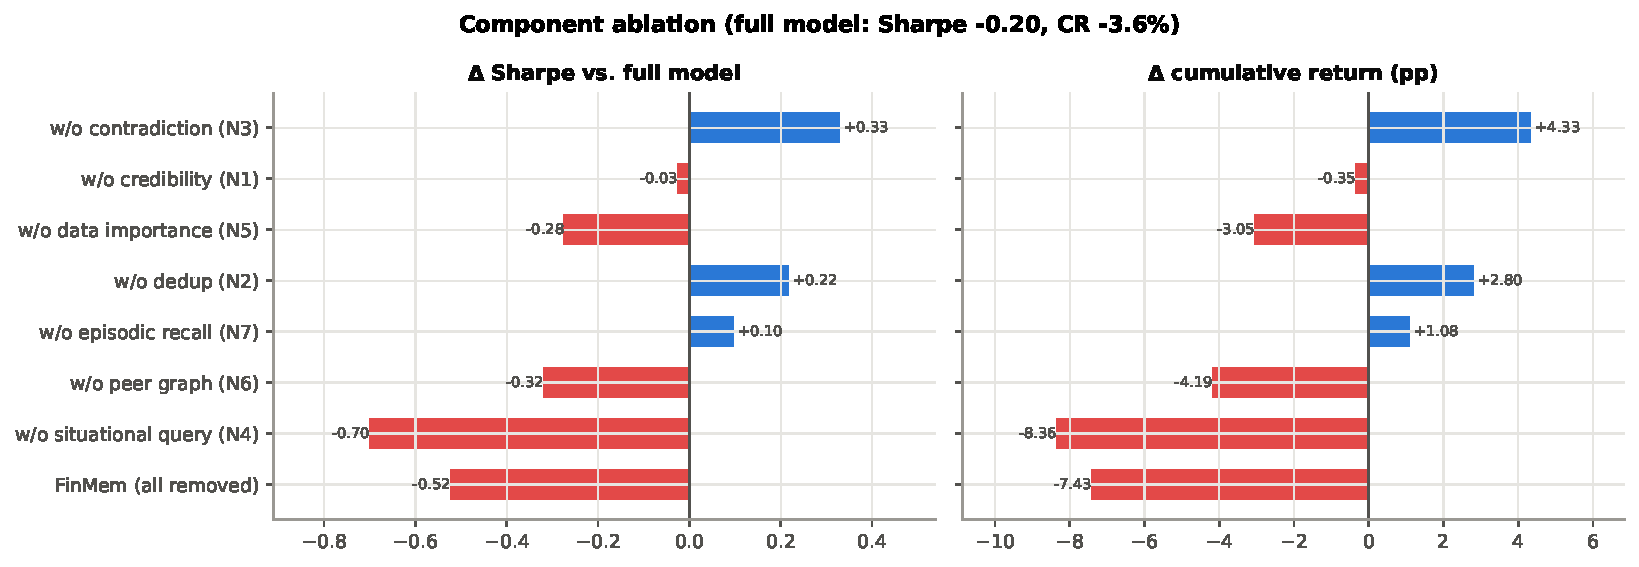
\includegraphics[width=\textwidth]{fig08_ablation.pdf}
\caption{Change in Sharpe ratio and cumulative return when a component is removed.}
\label{fig:ablation}
\end{figure}

\subsection{Sensitivity analyses}
\paragraph{Working-memory capacity.} Table~\ref{tab:topk} and Figure~\ref{fig:topk} vary $K$. Performance is non-monotonic and the spread across $K$ (FinMem: $-0.72$ to $2.27$) is larger than the difference between architectures at $K=5$; with $K=1$ FinMem performs best of all configurations. We kept FinMem's $K=5$ fixed in advance and report this sensitivity as a warning: choosing $K$ on the test period would be a form of selection bias~\cite{bailey2014deflated}.

\begin{table}[ht]
\centering
\caption{Sensitivity to working-memory capacity (top-$K$ per layer), Sharpe ratio, rolling protocol.}
\label{tab:topk}
\begin{tabular}{lrrrr}
\hline
System & $K=1$ & $K=3$ & $K=5$ & $K=10$ \\
\hline
FinMem & 2.27 & 0.11 & -0.72 & -0.38 \\
Ours & 0.51 & -0.64 & -0.20 & -0.46 \\
\hline
\end{tabular}
\end{table}


\begin{figure}[H]
\centering
\begin{minipage}{0.48\textwidth}\centering
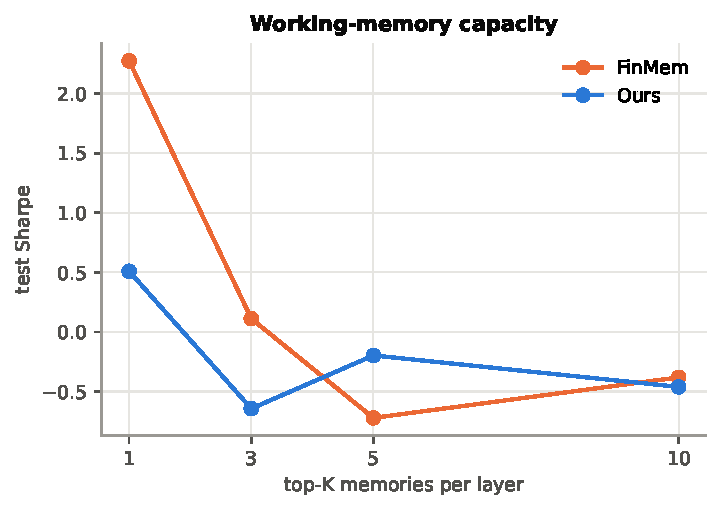
\includegraphics[width=\textwidth]{fig09_topk.pdf}
\caption{Sharpe ratio versus top-$K$.}
\label{fig:topk}
\end{minipage}\hfill
\begin{minipage}{0.48\textwidth}\centering
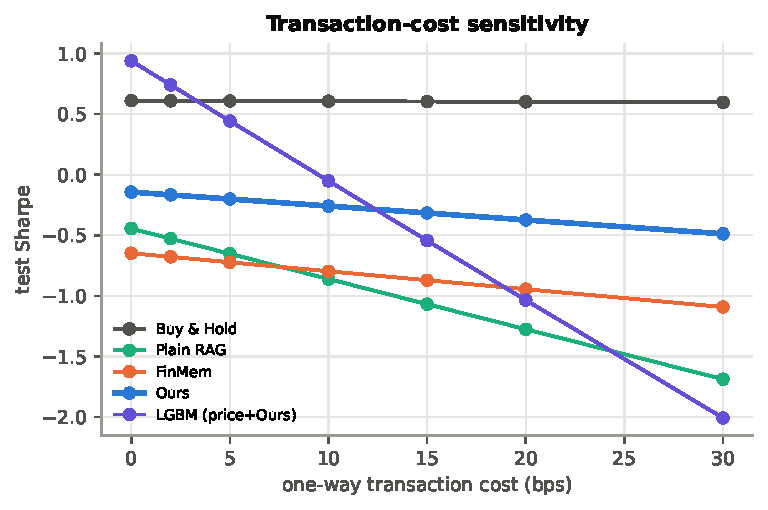
\includegraphics[width=\textwidth]{fig10_costs.pdf}
\caption{Sharpe ratio versus transaction cost.}
\label{fig:costs}
\end{minipage}
\end{figure}

\paragraph{Transaction costs.} The memory policies trade rarely (turnover 0.06--0.16 position units per day). Ours remains the best memory at every cost level from 0 to 30\,bps, while FinMem overtakes Plain RAG above about 8\,bps because Plain RAG trades twice as often (Figure~\ref{fig:costs}). The high-turnover LightGBM with memory features falls from a Sharpe ratio of 0.94 without costs to $-2.0$ at 30\,bps.

\paragraph{Fixed-split protocol.} Under the single test window of FinMem's design (Table~\ref{tab:fixed}), the ranking reverses: FinMem's validation-selected threshold ($\theta=0.4$) makes it almost always long, which matches buy-and-hold in a rising market, while ours, with $\theta=0.15$, trades more and loses. On the validation period itself ours had the highest IC of the three memories (0.087 versus 0.065 for FinMem and $-0.006$ for Plain RAG), and this ranking did not survive into the test period. The contrast between the two protocols is the strongest argument for walk-forward evaluation of trading agents.

\begin{table}[ht]
\centering
\caption{Ten-stock portfolio, fixed-split protocol (test 2026-05-01 to 2026-10-26, 123 sessions).}
\label{tab:fixed}
\small
\begin{tabular}{lrrrrrrr}
\hline
Strategy & CR (\%) & Sharpe & Sortino & Ann. Vol (\%) & MDD (\%) & Win (\%) & Turnover \\
\hline
Buy \& Hold & 6.79 & 0.68 & 1.07 & 23.89 & -13.19 & 51.2 & 0.01 \\
Momentum (1d) & -16.22 & -2.06 & -3.21 & 16.89 & -18.35 & 46.3 & 0.56 \\
TS-Momentum (20d) & -13.64 & -1.38 & -2.02 & 20.30 & -26.85 & 49.6 & 0.16 \\
Mean-Reversion (5d) & \textbf{14.97} & \textbf{1.80} & 2.47 & 16.67 & \textbf{-5.29} & 53.7 & 0.30 \\
MA-Crossover & -7.86 & -0.83 & -1.15 & 18.23 & -19.62 & 49.6 & 0.17 \\
Daily News Sentiment & -8.76 & -1.41 & -2.12 & 12.76 & -12.67 & 42.3 & 0.35 \\ \hline
LogReg (price) & -4.47 & -0.35 & -0.56 & 20.86 & -11.90 & 49.6 & 0.05 \\
LGBM (price) & -8.55 & -0.95 & -1.70 & 17.61 & -21.03 & 48.0 & 0.60 \\
LGBM (price+FinMem) & 11.95 & 1.46 & \textbf{2.68} & 16.76 & -6.03 & 48.8 & 0.59 \\
LGBM (price+Ours) & -8.18 & -0.94 & -1.48 & 16.98 & -16.66 & 51.2 & 0.64 \\ \hline
Plain RAG & -10.64 & -1.34 & -2.02 & 16.25 & -18.05 & 46.3 & 0.11 \\
FinMem & 5.25 & 0.67 & 1.10 & 18.08 & -10.60 & 52.0 & 0.01 \\
Ours & -15.37 & -2.21 & -3.13 & 14.97 & -17.95 & 44.7 & 0.07 \\
\hline
\end{tabular}
\end{table}


\subsection{Retrieval diagnostics}
Figure~\ref{fig:retrieval} characterises the retrieved context. Flat retrieval returns the most redundant context (mean pairwise similarity 0.45, against 0.36 for FinMem and 0.37 for ours) and only same-day news; FinMem's context is the oldest (mean age 58 days, dominated by filings and promoted items); ours retrieves fresher memories (26 days) while still covering all three layers. Over the run our memory merged 2{,}260 re-reported stories and retired 667 contradicted ones (Table~\ref{tab:icops}, Figure~\ref{fig:memdyn}). Learned credibility (Figure~\ref{fig:cred}) stays close to 0.5 for most categories; analyst notes (0.45) are the least reliable next-day guide and options-activity reports the most (0.64, but with only 80 observations).

\begin{figure}[H]
\centering
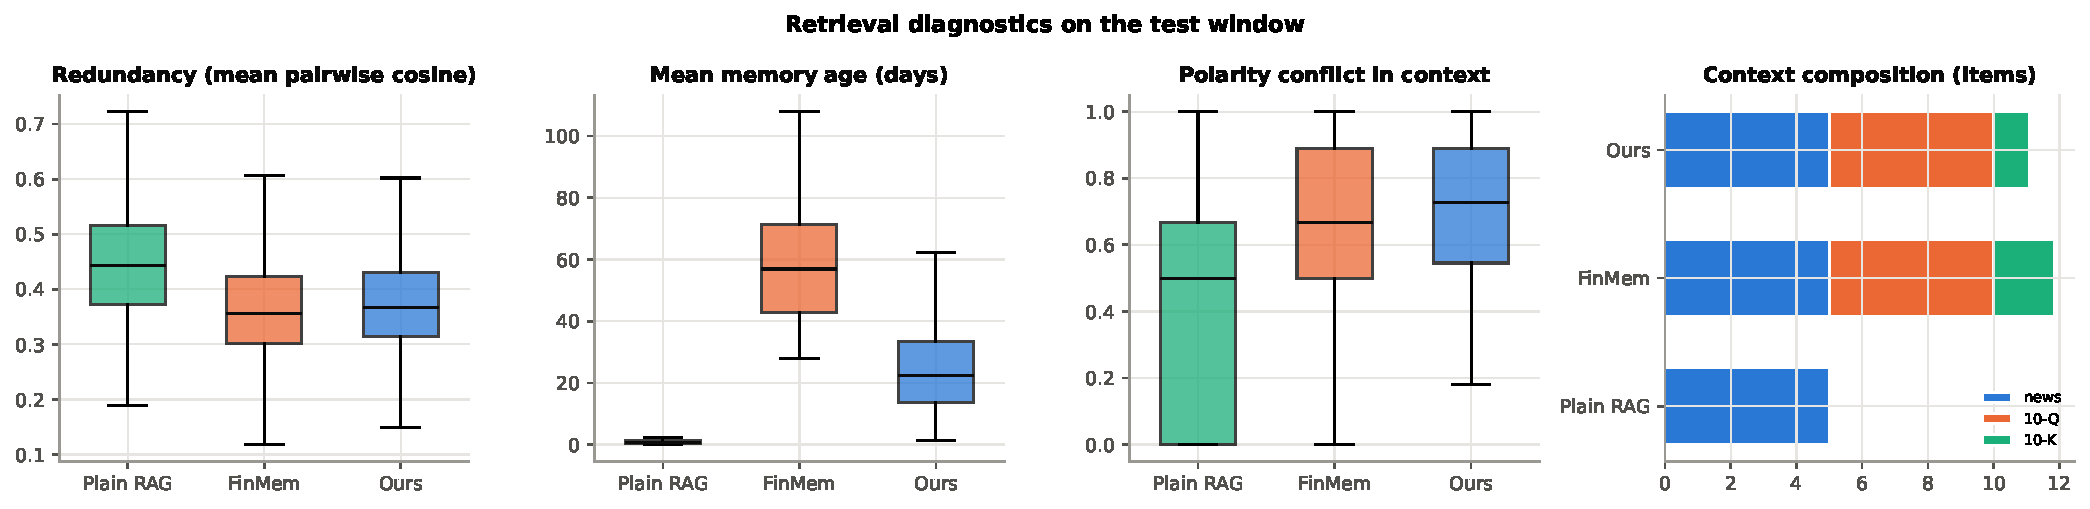
\includegraphics[width=\textwidth]{fig13_retrieval_diagnostics.pdf}
\caption{Retrieval diagnostics: redundancy, age, polarity conflict and layer composition of the retrieved context.}
\label{fig:retrieval}
\end{figure}

\begin{figure}[H]
\centering
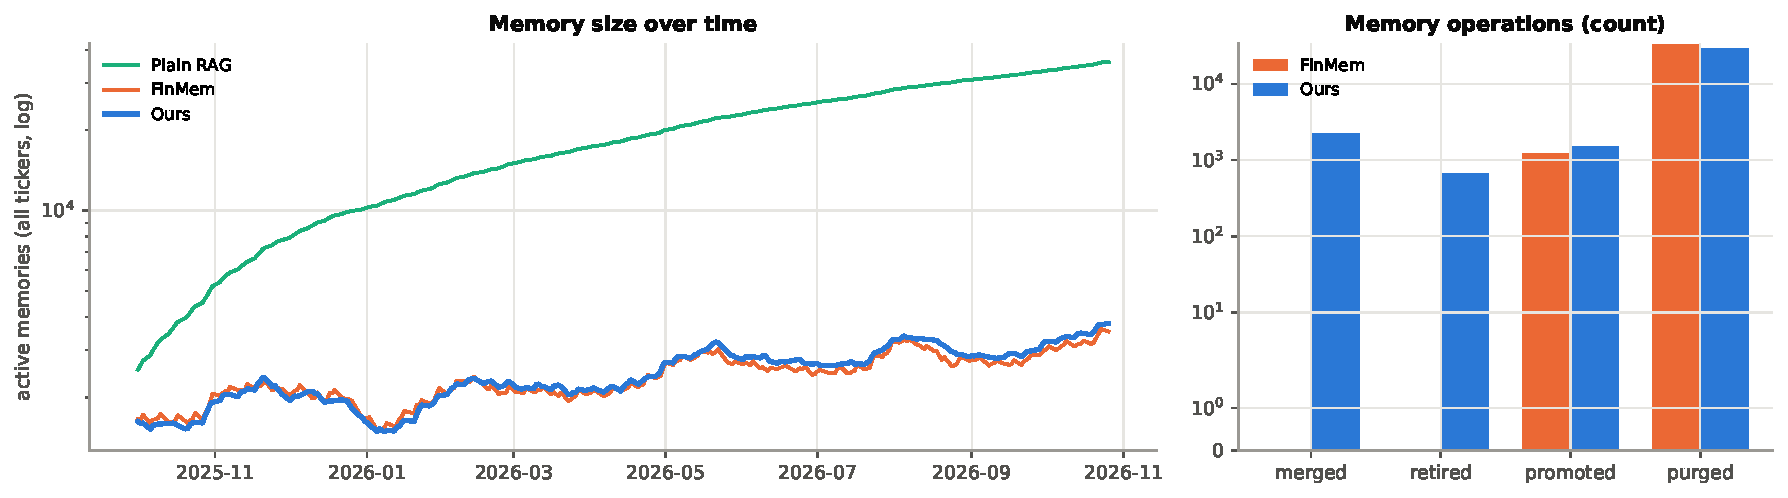
\includegraphics[width=\textwidth]{fig18_memory_dynamics.pdf}
\caption{Active memory size over time and memory operations.}
\label{fig:memdyn}
\end{figure}

\begin{figure}[H]
\centering
\begin{minipage}{0.55\textwidth}\centering
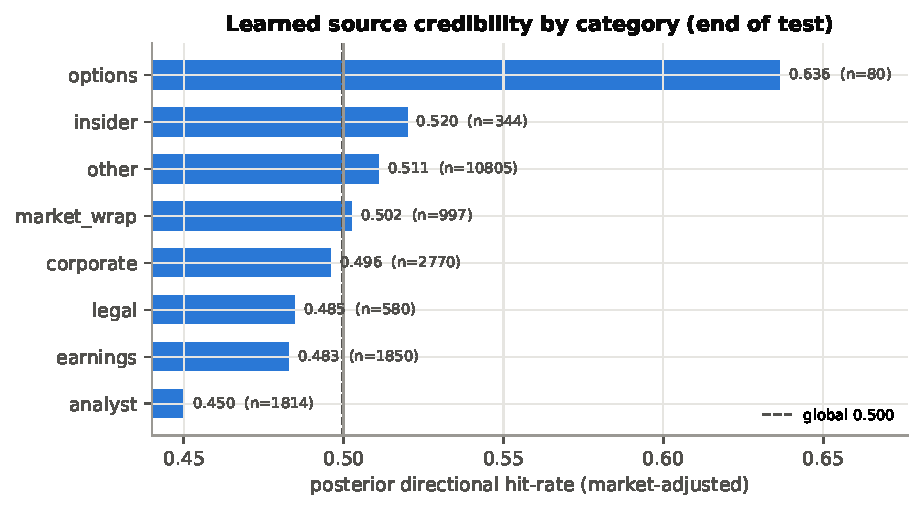
\includegraphics[width=\textwidth]{fig14_credibility.pdf}
\caption{Learned category credibility (N1).}
\label{fig:cred}
\end{minipage}\hfill
\begin{minipage}{0.42\textwidth}\centering
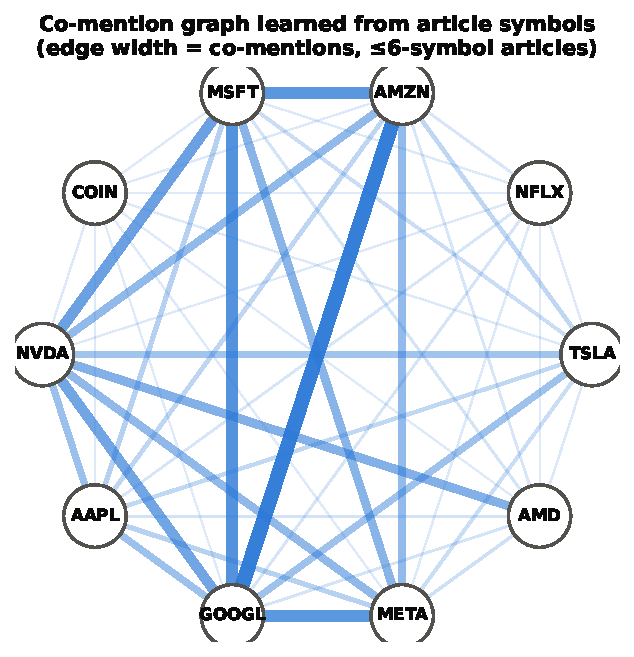
\includegraphics[width=\textwidth]{fig19_peer_graph.pdf}
\caption{Co-mention graph used by N6.}
\label{fig:peers}
\end{minipage}
\end{figure}

\subsection{LLM backbones}
Table~\ref{tab:llm} and Figure~\ref{fig:llm} report the LLM experiment: three free Groq backbones read the context retrieved by each memory (or none) for FinMem's five stocks over the last 50 test sessions (17 August -- 26 October 2026), 2{,}250 decisions in total, all parsed successfully. With every backbone, the context from our memory gives a higher return and a smaller drawdown than FinMem's context: $+2.55\%$ versus $-12.00\%$ (gpt-oss-120b), $+1.33\%$ versus $-10.70\%$ (gpt-oss-20b) and $-1.34\%$ versus $-4.79\%$ (qwen3.8-27b), with maximum drawdowns roughly halved ($-6.3/-4.8/-5.8\%$ versus $-14.7/-10.7/-10.7\%$). Pooled over backbones, the advantage over FinMem is 20.9 basis points per day but not significant (Wilcoxon $p=0.12$), and the advantage over the memory-less prompt is small and inconsistent (qwen3.8-27b does best without memory). None of the configurations clearly beats buy-and-hold over this short window ($+3.9\%$). In the action mix, our context (which includes the episodic-recall warning) makes gpt-oss-20b and qwen3.8-27b hold more often than FinMem's context (73\% and 92\% versus 61\% and 70\% Hold), while gpt-oss-120b holds equally often with both (45--46\%), so the gain is not only a matter of trading less. The three backbones agree on the same action in only 26\% of the decisions, so the choice of backbone is itself a large source of variance.

\begin{table}[ht]
\centering
\caption{LLM backbones deciding from the same retrieved memory (FinMem-style prompt, temperature 0, single trial), FinMem's five stocks, last 50 test sessions, 250 decisions per row.}
\label{tab:llm}
\small
\begin{tabular}{llrrrc}
\hline
Backbone & Memory & CR (\%) & Sharpe & MDD (\%) & Buy/Sell/Hold (\%) \\
\hline
gpt-oss-120b & No-Memory & -3.61 & -0.73 & -8.18 & 9/43/48 \\
gpt-oss-120b & FinMem & -12.00 & -3.15 & -14.74 & 28/26/46 \\
gpt-oss-120b & Ours & 2.55 & 0.74 & -6.33 & 28/27/45 \\
\hline
gpt-oss-20b & No-Memory & -6.59 & -1.74 & -7.14 & 6/56/39 \\
gpt-oss-20b & FinMem & -10.70 & -2.47 & -10.74 & 26/13/61 \\
gpt-oss-20b & Ours & 1.33 & 0.45 & -4.82 & 20/7/73 \\
\hline
qwen3.8-27b & No-Memory & 3.48 & 0.78 & -7.21 & 24/0/76 \\
qwen3.8-27b & FinMem & -4.79 & -1.15 & -10.73 & 16/13/70 \\
qwen3.8-27b & Ours & -1.34 & -0.27 & -5.77 & 6/2/92 \\
\hline
\multicolumn{6}{p{0.9\textwidth}}{\footnotesize Pooled over backbones: Ours vs FinMem: +20.9 bps/day, Wilcoxon $p=0.123$; Ours vs No-Memory: +6.1 bps/day, Wilcoxon $p=0.508$.} \\
\multicolumn{6}{p{0.9\textwidth}}{\footnotesize Buy \& Hold over the same window: CR 3.89\%.} \\
\hline
\end{tabular}
\end{table}


\begin{figure}[H]
\centering
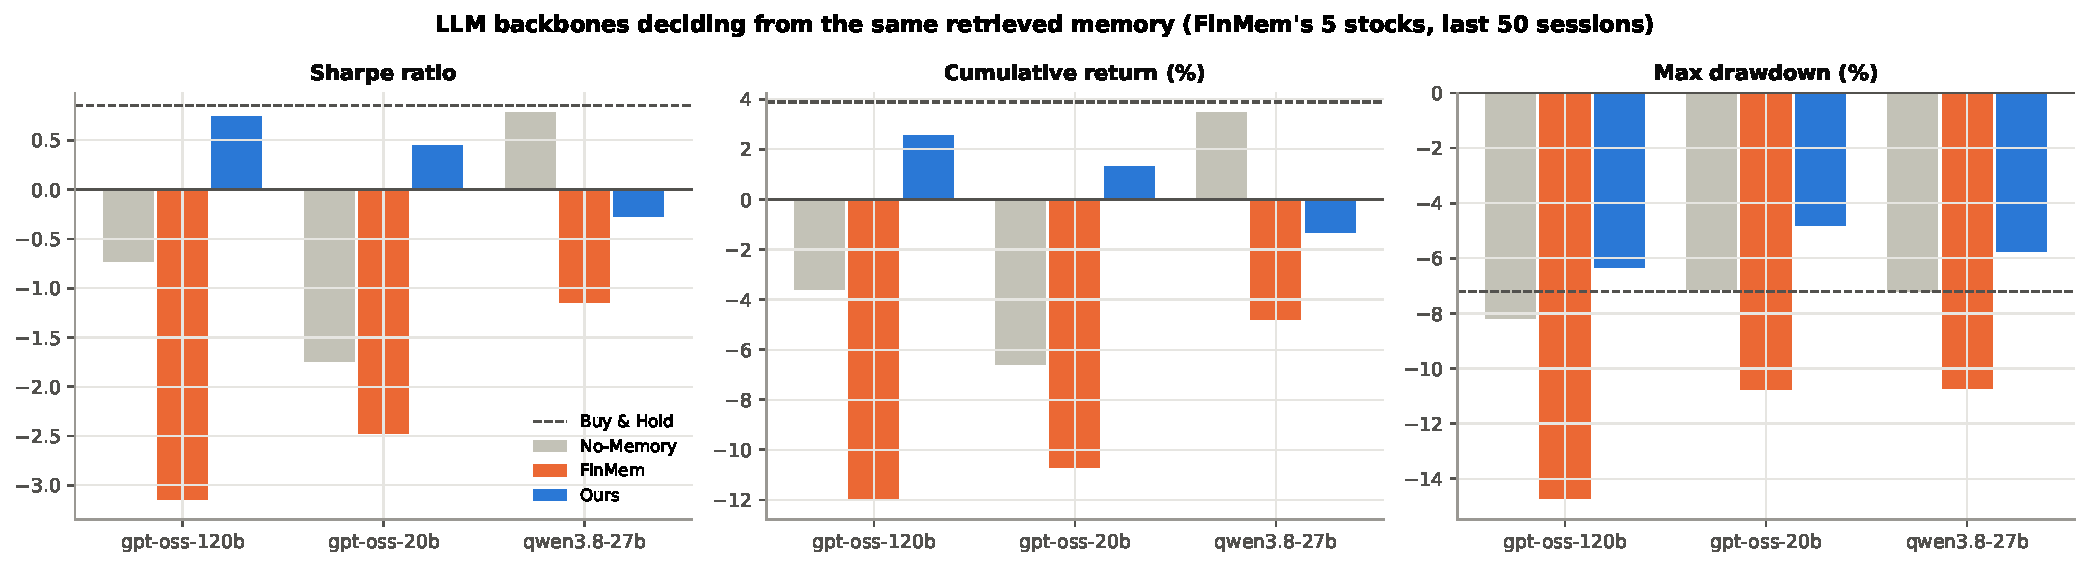
\includegraphics[width=\textwidth]{fig20_llm_backbones.pdf}
\caption{LLM backbones deciding from the same retrieved memory.}
\label{fig:llm}
\end{figure}

\section{Extension Models: Deep Learning, Reinforcement Learning and Pattern Matching}
\label{sec:ext-results}
The main study compares memory architectures with rule and gradient-boosting baselines. To test whether its conclusions depend on the model family, we evaluated five more models on exactly the same protocol (Section~\ref{sec:ext-design}): a GRU, a Transformer on price features, the same Transformer with our memory features, a tabular Q-learning agent and a nearest-neighbour pattern model, plus two exploratory combinations defined after the main results were known. The whole extension run (33 monthly network fits per model, ten Q-learning agents and ten analogue back-tests) took 531 seconds on the laptop CPU.

\subsection{Overall comparison}
Table~\ref{tab:ext-main} and Figures~\ref{fig:zoo-equity}--\ref{fig:zoo-sharpe} summarise all models. Four observations stand out.
\begin{enumerate}
  \item \textbf{A small Transformer on price features is competitive.} It earned $+11.6\%$ (Sharpe $0.95$) with the smallest drawdown of all models ($-7.9\%$), roughly on par with buy-and-hold ($+11.2\%$, $0.61$) and below the price-only LightGBM ($+19.4\%$, $1.15$). The GRU was weaker ($0.28$).
  \item \textbf{Adding news-memory features hurts learned models.} Giving the same Transformer our memory features lowered its Sharpe from $0.95$ to $0.09$ and deepened its drawdown from $-7.9\%$ to $-18.0\%$. This replicates, with a completely different model class, the main study's finding that memory features lower LightGBM's Sharpe (1.15 to 0.44). The evidence that next-day information in news memory is close to zero is therefore not specific to one model.
  \item \textbf{Reinforcement learning learned little that generalises.} The Q-learning agent earned $+4.4\%$ (Sharpe $0.39$), below buy-and-hold. It held a (long-only) position on 54\% of stock-days and its portfolio has a market beta of $0.84$, so its result largely follows the market.
  \item \textbf{The pattern model had the highest Sharpe ($1.45$), but the result is fragile} (Section~\ref{sec:analogs}): its default settings happen to be the best of nine combinations, and five of the nine are negative.
\end{enumerate}
None of these differences is statistically significant (Table~\ref{tab:ext-tests}): all 95\% bootstrap intervals for the Sharpe difference against buy-and-hold, LightGBM and our memory contain zero, and the smallest Wilcoxon $p$-value is $0.085$ (the exploratory model vote against our memory). The exploratory risk overlay, which keeps LightGBM's position but stays in cash when our memory abstains, cut LightGBM's drawdown from $-17.2\%$ to $-11.6\%$ and its volatility from 19\% to 11\% at the cost of return (Sharpe $1.03$ versus $1.15$), consistent with the earlier observation that episodic recall works more as a risk control than as a signal; because it was designed after the main results, it is a hypothesis for future work, not a finding.

\begin{table}[H]
\centering
\small
\caption{Extension models on the primary rolling protocol (10 stocks, 227 test days, 5 bps costs). Beta and alpha are against SPY; IC is the pooled Spearman correlation of the model's signal with the next-day return. $^{*}$Exploratory combinations defined after the main results were known.}
\label{tab:ext-main}
\resizebox{\textwidth}{!}{%
\begin{tabular}{lrrrrrrrr}
\toprule
Model & CR & Sharpe & Sortino & MDD & Vol & $\beta$ & $\alpha$/yr & IC \\
\midrule
Buy \& Hold & +11.2\% & +0.61 & +0.96 & -16.5\% & 24\% & +1.62 & -10.8\% & -- \\
LGBM (price) & +19.4\% & +1.15 & +1.91 & -17.2\% & 19\% & -0.11 & +23.2\% & -- \\
LogReg (price) & -21.5\% & -1.39 & -2.13 & -29.7\% & 18\% & -0.17 & -22.7\% & -- \\
GRU (price) & +3.0\% & +0.28 & +0.43 & -11.8\% & 16\% & +0.21 & +1.3\% & +0.017 \\
\textbf{Transformer (price)} & +11.6\% & +0.95 & +1.41 & -7.9\% & 14\% & -0.12 & +14.9\% & +0.024 \\
Transformer (price+memory) & +0.2\% & +0.09 & +0.15 & -18.0\% & 16\% & +0.07 & +0.5\% & +0.023 \\
\textbf{RL Q-learning} & +4.4\% & +0.39 & +0.58 & -14.7\% & 15\% & +0.84 & -7.2\% & -- \\
Pattern analogs (kNN) & +17.7\% & +1.45 & +2.15 & -6.4\% & 13\% & +0.49 & +11.2\% & +0.034 \\
\textbf{Ours} & -3.6\% & -0.20 & -0.30 & -15.2\% & 15\% & -0.33 & +2.3\% & -- \\
FinMem & -11.0\% & -0.72 & -1.03 & -19.7\% & 16\% & +0.64 & -21.7\% & -- \\
\midrule
LGBM + memory risk overlay$^{*}$ & +10.4\% & +1.03 & +1.60 & -11.6\% & 11\% & +0.06 & +10.6\% & +0.017 \\
Model vote (LGBM, Transformer, Ours)$^{*}$ & +14.9\% & +1.09 & +1.58 & -14.9\% & 15\% & -0.29 & +21.2\% & +0.036 \\
\bottomrule
\end{tabular}
}
\end{table}


\begin{figure}[H]
\centering
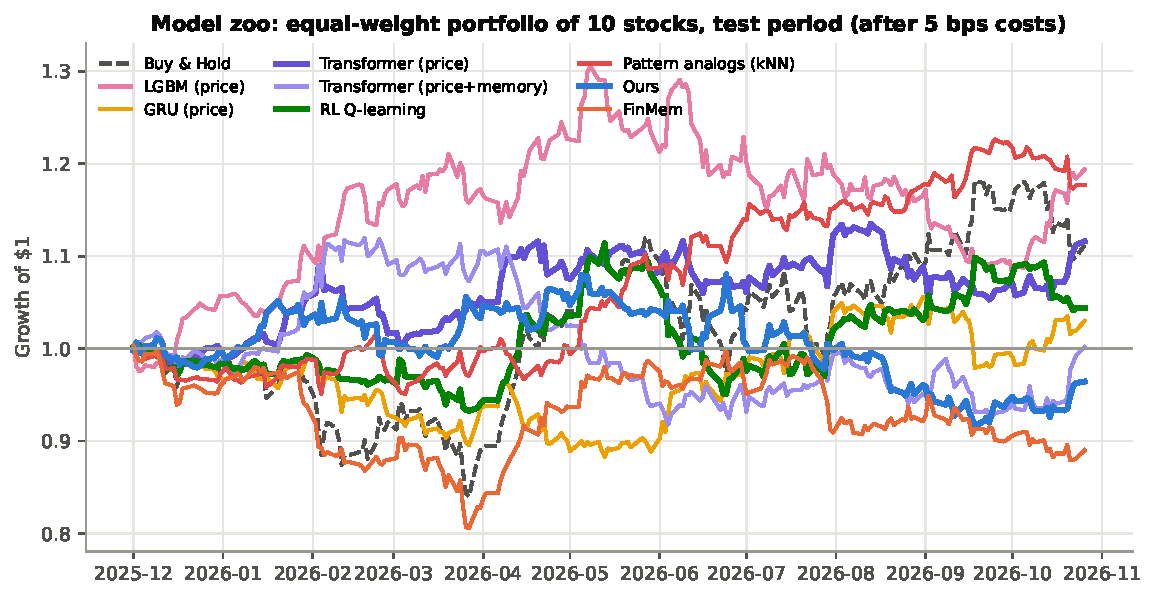
\includegraphics[width=\textwidth]{fig21_model_zoo_equity.pdf}
\caption{Growth of \$1 for all model families on the same 10-stock, 227-day test (equal weight, after costs).}
\label{fig:zoo-equity}
\end{figure}
\begin{figure}[H]
\centering
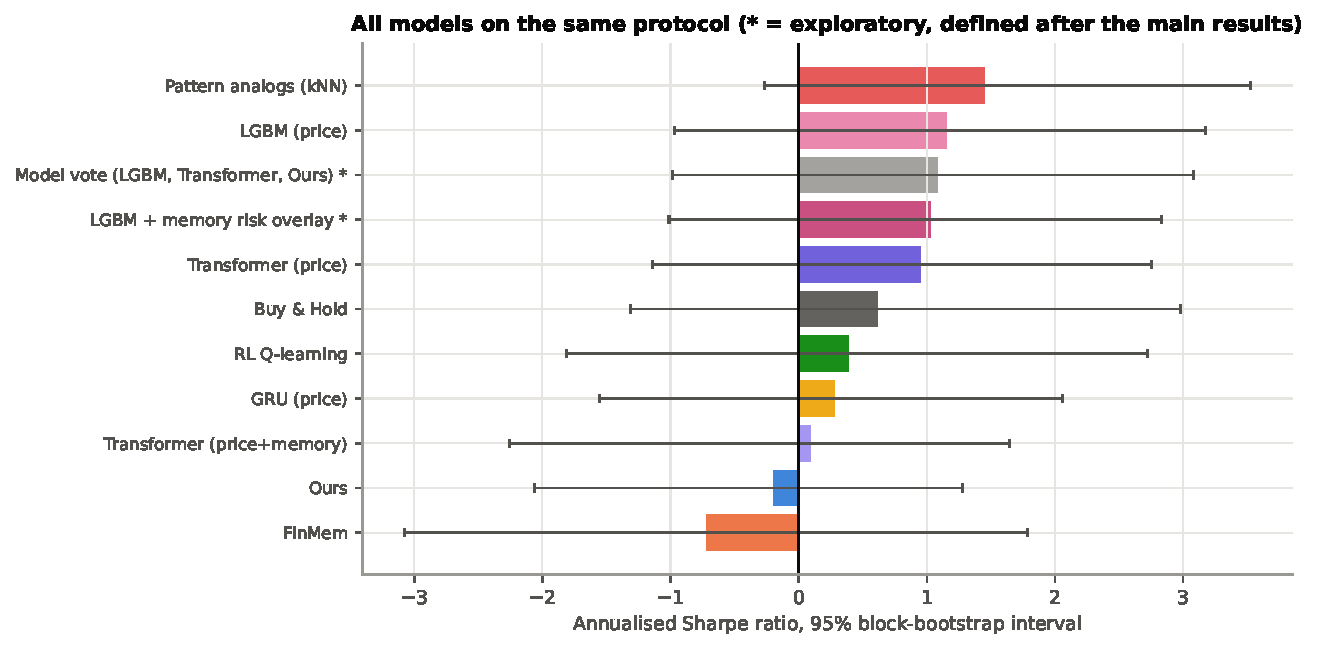
\includegraphics[width=\textwidth]{fig22_model_zoo_sharpe.pdf}
\caption{Sharpe ratio of every model with its 95\% moving-block bootstrap interval. All intervals overlap zero and each other.}
\label{fig:zoo-sharpe}
\end{figure}

\begin{figure}[!htbp]
\centering
\appshot{app_zoo_paper.png}
\caption{The same comparison in the application's Research lab.}
\label{fig:ui-zoo}
\end{figure}

\begin{table}[H]
\centering
\small
\caption{Pairwise comparisons of the extension models: $\Delta$Sharpe with 95\% block-bootstrap interval and Wilcoxon signed-rank $p$ on daily portfolio returns, against buy-and-hold, the price-only LightGBM and our memory.}
\label{tab:ext-tests}
\resizebox{\textwidth}{!}{%
\begin{tabular}{lrrrrrr}
\toprule
Model & \multicolumn{2}{c}{vs Buy \& Hold} & \multicolumn{2}{c}{vs LGBM (price)} & \multicolumn{2}{c}{vs Ours} \\
 & $\Delta$Sharpe [CI] & $p$ & $\Delta$Sharpe [CI] & $p$ & $\Delta$Sharpe [CI] & $p$ \\
\midrule
GRU (price) & -0.33 [-3.5, +2.5] & 0.72 & -0.87 [-3.7, +1.9] & 0.71 & +0.48 [-1.9, +3.2] & 0.58 \\
Transformer (price) & +0.34 [-2.7, +3.0] & 0.73 & -0.20 [-2.8, +2.1] & 0.82 & +1.15 [-0.9, +3.2] & 0.12 \\
Transformer (price+memory) & -0.52 [-4.7, +2.5] & 0.78 & -1.06 [-4.2, +1.2] & 0.95 & +0.29 [-2.3, +2.4] & 0.58 \\
RL Q-learning & -0.22 [-1.4, +1.0] & 0.49 & -0.76 [-3.7, +2.4] & 0.41 & +0.58 [-2.0, +3.8] & 0.77 \\
Pattern analogs (kNN) & +0.84 [-2.0, +3.3] & 0.50 & +0.30 [-2.7, +3.7] & 0.78 & +1.65 [-0.4, +4.5] & 0.24 \\
LGBM + memory risk overlay$^{*}$ & +0.42 [-2.9, +3.1] & 0.82 & -0.12 [-1.5, +1.2] & 0.41 & +1.23 [-1.2, +3.9] & 0.59 \\
Model vote (LGBM, Transformer, Ours)$^{*}$ & +0.48 [-2.9, +3.3] & 0.82 & -0.06 [-2.0, +1.6] & 0.98 & +1.28 [-0.4, +3.1] & 0.09 \\
\bottomrule
\end{tabular}
}
\end{table}


\subsection{What the neural networks learned}
Figure~\ref{fig:deep-training} looks inside the networks. On the held-out last 15\% of each training set, the validation loss never fell clearly below that of a coin flip ($\ln 2 = 0.693$): the best validation losses averaged $0.683$ (GRU), $0.689$ (Transformer) and $0.693$ (Transformer with memory), and early stopping chose epoch 7 on average for the Transformer. The training loss of the memory-augmented Transformer fell much faster than that of the price-only one while its validation loss rose, the signature of over-fitting to extra features that do not generalise. The attention of the decision day over the 20-day window is almost uniform (the dotted line marks $1/20$); the price-only Transformer puts slightly more weight on the most recent five days (25.6\% versus 24.8\% on the oldest five). In short, the networks found only a faint next-day signal, and their trading results should be read with that in mind.

\begin{figure}[H]
\centering
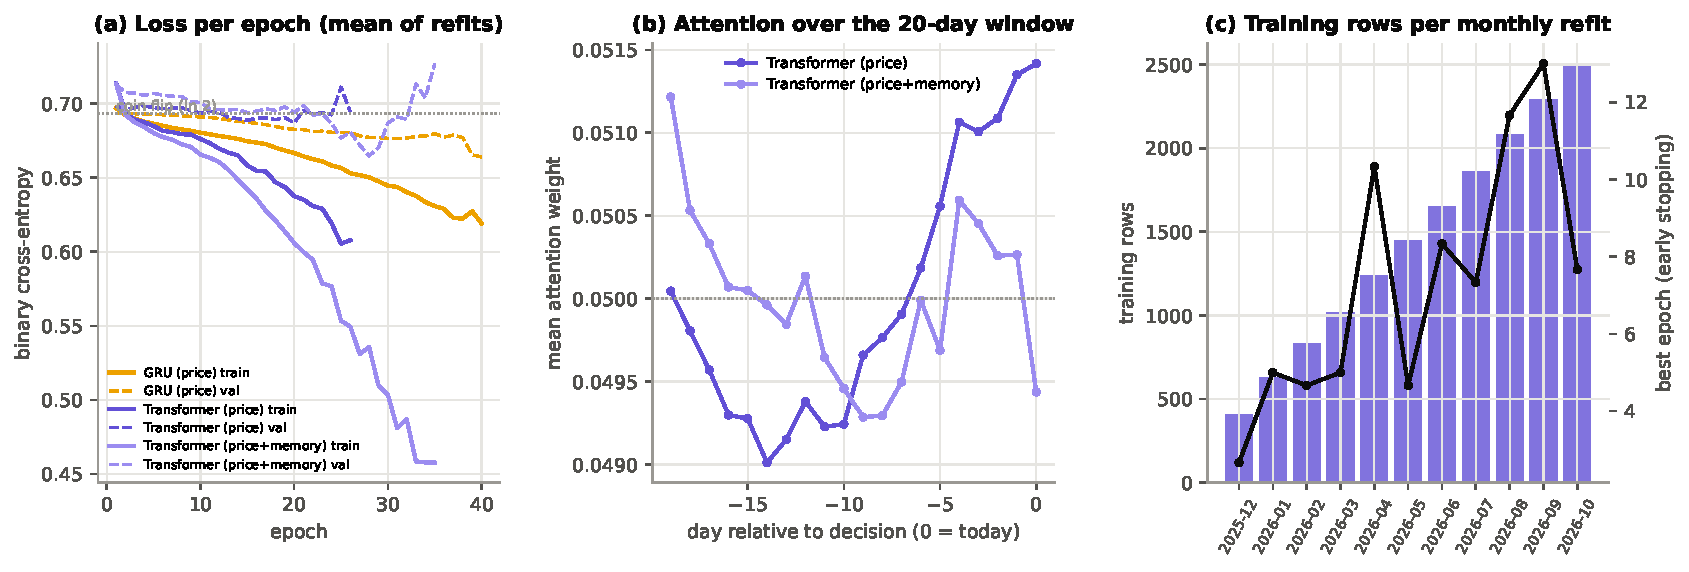
\includegraphics[width=\textwidth]{fig23_deep_training.pdf}
\caption{Deep models: (a) training and validation loss per epoch averaged over refits; (b) attention of the decision day over the 20-day window; (c) size of the training set at each monthly refit and the epoch chosen by early stopping.}
\label{fig:deep-training}
\end{figure}

\subsection{Reinforcement-learning agent}
Figure~\ref{fig:rl} shows the Q-learning agent. Its pre-training reward per decision fluctuates between passes instead of rising steadily, because each pass explores differently and daily rewards are dominated by noise. After 30 passes and the online updates of the test window, the agent had learned from 42{,}320 transitions and visited 25 of the 36 possible situations. Per stock it beat buy-and-hold on four stocks, AAPL (Sharpe $2.03$ versus $1.05$), AMD ($2.09$ versus $1.86$), MSFT and COIN, and lost on the other six, most clearly on NVDA, GOOGL and TSLA (Table~\ref{tab:ext-per-ticker}). The learned policy (panel c) is mostly ``stay invested'', with a strong exception: when the stock has fallen over five days, is below its 20-day average and RSI is neutral, the agent prefers to sell what it holds. The application exposes the same agent per stock, with its Q-table, its decision log and the reward of every decision (Figure~\ref{fig:ui-rl}).

\begin{figure}[H]
\centering
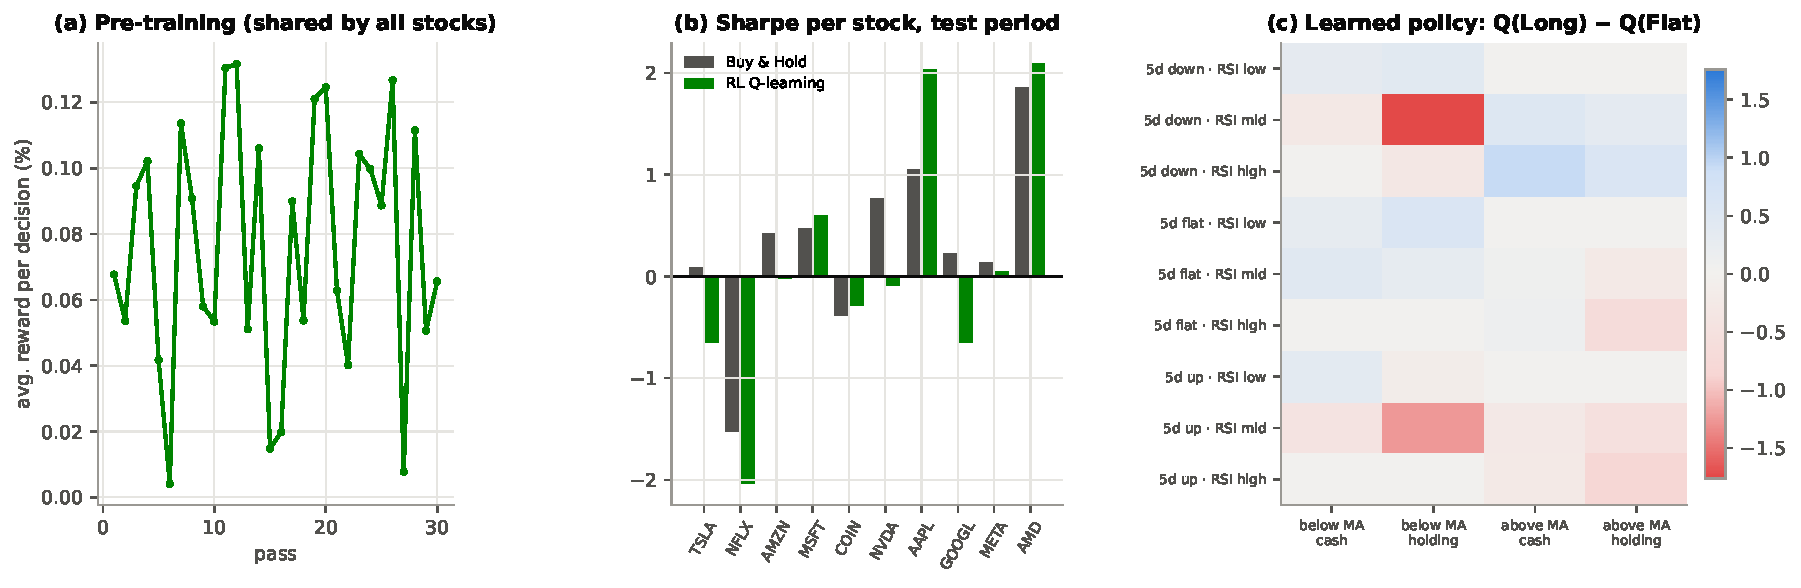
\includegraphics[width=\textwidth]{fig24_rl_agent.pdf}
\caption{Q-learning agent: (a) average reward per decision in each pre-training pass; (b) Sharpe ratio per stock against buy-and-hold in the test period; (c) learned preference for holding over cash, $Q(\text{Long})-Q(\text{Flat})$, in each market situation (averaged over the ten stock-specific agents).}
\label{fig:rl}
\end{figure}

\begin{table}[H]
\centering
\small
\caption{Sharpe ratio per stock in the test period.}
\label{tab:ext-per-ticker}
\resizebox{\textwidth}{!}{%
\begin{tabular}{lrrrrrrrrrr}
\toprule
Model & TSLA & NFLX & AMZN & MSFT & COIN & NVDA & AAPL & GOOGL & META & AMD \\
\midrule
Buy \& Hold & +0.09 & -1.52 & +0.42 & +0.47 & -0.38 & +0.77 & +1.05 & +0.23 & +0.13 & +1.86 \\
LGBM & +1.38 & -0.06 & +0.69 & -1.22 & +0.68 & +2.13 & -0.92 & +0.57 & +0.18 & +0.63 \\
GRU & -0.72 & +0.03 & +1.21 & -0.90 & +0.42 & +1.16 & +0.02 & -0.28 & +0.54 & -0.28 \\
Transf. & +0.69 & +0.50 & +0.02 & +0.53 & +0.23 & +0.36 & +0.18 & -0.10 & +0.52 & +0.16 \\
Transf.+mem & -0.79 & +1.08 & -0.65 & -1.43 & +0.36 & +1.47 & -0.91 & -0.48 & +2.20 & -0.77 \\
RL Q-learning & -0.65 & -2.04 & -0.02 & +0.59 & -0.28 & -0.09 & +2.03 & -0.65 & +0.05 & +2.09 \\
Analogs & -2.29 & +0.82 & +0.75 & -0.10 & +1.26 & +0.96 & +0.35 & +0.22 & +0.82 & +1.13 \\
Ours & -1.39 & +2.33 & -0.52 & +0.64 & +0.08 & -0.64 & +0.66 & +0.27 & -1.66 & +0.12 \\
FinMem & -0.99 & +0.26 & -0.54 & +0.05 & -1.73 & +0.84 & +0.56 & -1.61 & +0.09 & +0.86 \\
\bottomrule
\end{tabular}
}
\end{table}


\subsection{Pattern analogues}
\label{sec:analogs}
Figure~\ref{fig:analogs} repeats the pattern model for every combination of pattern length (10, 20, 40 days) and look-ahead (5, 10, 20 days) on a common test period. Averaged over the ten stocks, five of the nine settings have a negative Sharpe ratio, two more are close to zero (0.01 and 0.04), and only one setting, the 20-day pattern with a 10-day look-ahead (0.50), beats the average buy-and-hold Sharpe ratio of 0.35; even that setting beats buy-and-hold on just 6 of 10 stocks. The default (20-day pattern, 10-day look-ahead, chosen for the application before any test) happens to be the best cell. We therefore do not claim that chart patterns predict returns: the strong portfolio result of Table~\ref{tab:ext-main} is the kind of outcome that the multiple-testing literature~\cite{harvey2016cross,bailey2014deflated} warns about. For a single stock the picture can be much worse; on TSLA alone the same settings lost $50\%$, and the forecasts were negatively correlated with what happened next (Figure~\ref{fig:ui-pattern}).

\begin{figure}[H]
\centering
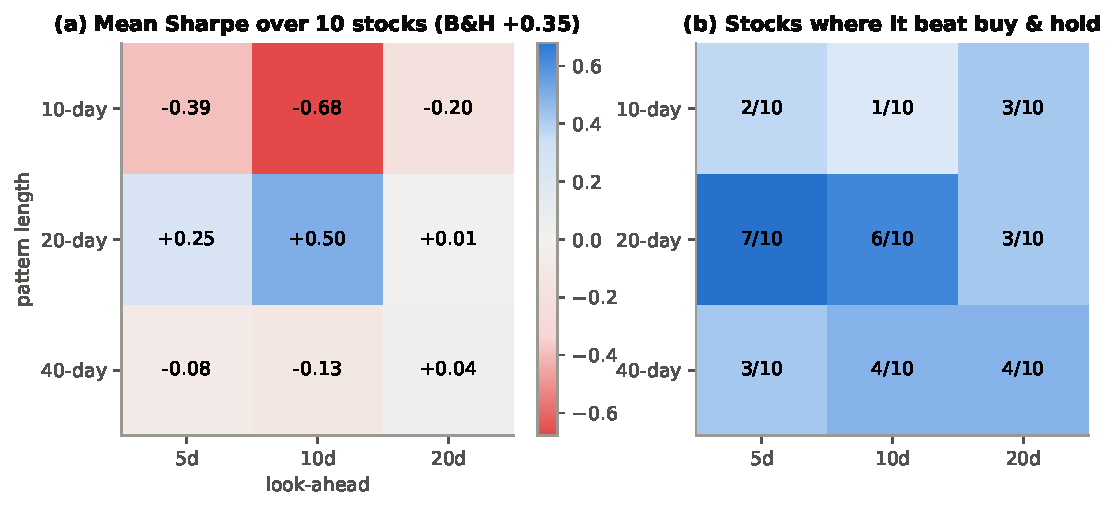
\includegraphics[width=\textwidth]{fig25_pattern_analogs.pdf}
\caption{Robustness of the pattern model: (a) mean Sharpe over the ten stocks for every pattern length and look-ahead, compared with buy-and-hold; (b) number of stocks on which each setting beat buy-and-hold.}
\label{fig:analogs}
\end{figure}
\begin{figure}[!htbp]
\centering
\appshot{app_pattern_paper_1.png}
\caption{Pattern finder in the application (TSLA): the latest 20-day pattern (bold) against the most similar past windows and what followed, the verdict, the daily back-test against buy-and-hold and the robustness grid.}
\label{fig:ui-pattern}
\end{figure}
\begin{figure}[!htbp]
\ContinuedFloat
\centering
\appshot{app_pattern_paper_2.png}
\caption[]{(continued)}
\end{figure}

\section{Portfolio Construction}
\label{sec:alloc-results}
The application advises how to split a budget across stocks (Section~\ref{sec:autopilot-design}). Table~\ref{tab:ext-alloc} and Figure~\ref{fig:alloc} compare the methods walk-forward: every 21 trading days the weights are recomputed from the previous 120 days only, with 80\% of the budget invested and at most 25\% per stock. Equal weight ($+10.7\%$, Sharpe $0.77$) and risk parity ($+9.2\%$, $0.75$) did better than minimum variance ($+5.1\%$, $0.51$), which concentrated in a few calm stocks (up to the 25\% cap in AAPL); all three had similar drawdowns of about $-12\%$. This matches the classic out-of-sample result that naive diversification is hard to beat~\cite{demiguel2009naive}. Investing the same 80\% in the S\&P 500 was the best risk-adjusted choice ($+10.0\%$, Sharpe $1.26$, drawdown $-7.1\%$): the ten technology-heavy stocks are highly correlated (Figure~\ref{fig:market-risk}), so splitting money among them diversifies less than holding the broad market. The application shows these numbers next to its suggestion so that the user sees this trade-off.

\begin{table}[H]
\centering
\small
\caption{Budget-split (portfolio construction) methods, walk-forward with monthly rebalancing, 80\% invested, at most 25\% of the budget per stock. SPY row: the same 80\% invested in the S\&P 500.}
\label{tab:ext-alloc}
\begin{tabular}{lrrrr}
\toprule
Method & Return & Volatility & Sharpe & MDD \\
\midrule
Risk parity (inverse volatility) & +9.2\% & 18\% & +0.75 & -11.7\% \\
Minimum variance & +5.1\% & 15\% & +0.51 & -11.6\% \\
Equal weight & +10.7\% & 20\% & +0.77 & -12.1\% \\
SPY (same exposure) & +10.0\% & 10\% & +1.26 & -7.1\% \\
\bottomrule
\end{tabular}
\end{table}


\begin{figure}[H]
\centering
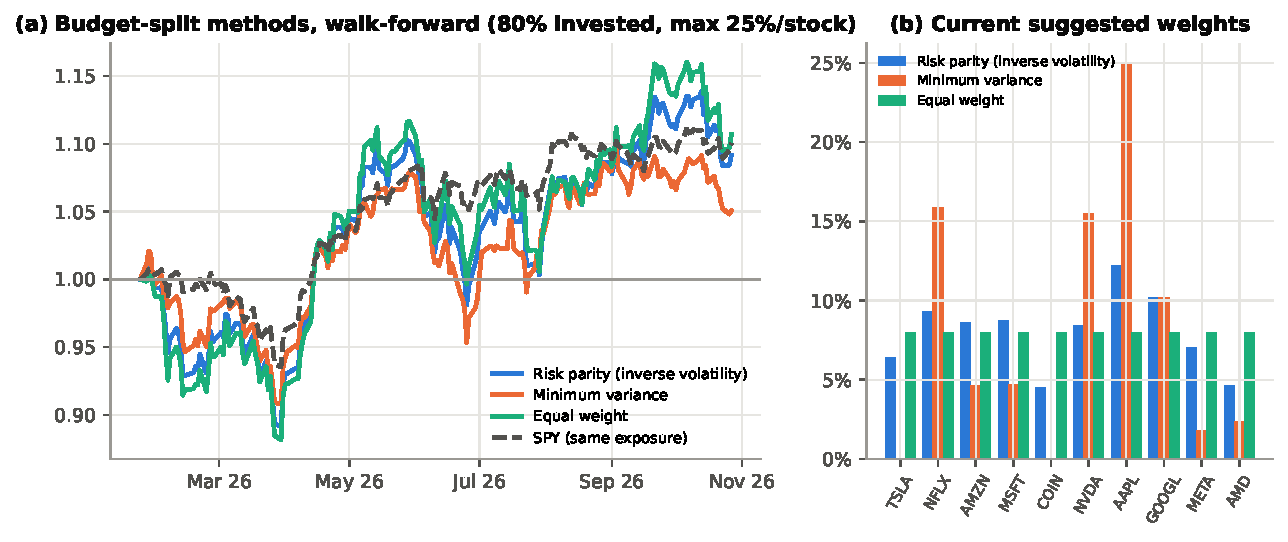
\includegraphics[width=\textwidth]{fig26_allocation.pdf}
\caption{Budget-split methods: (a) walk-forward growth with monthly rebalancing; (b) weights each method suggests today.}
\label{fig:alloc}
\end{figure}
\begin{figure}[!htbp]
\centering
\appshot{app_split_paper_1.png}
\caption{Budget split in the application: method choice, suggested amounts per stock with the trades needed to reach them, plan statistics and the walk-forward comparison.}
\label{fig:ui-split}
\end{figure}
\begin{figure}[!htbp]
\ContinuedFloat
\centering
\appshot{app_split_paper_2.png}
\caption[]{(continued)}
\end{figure}

\section{Robustness and Statistical Power}
\label{sec:robust}

\subsection{Market exposure (CAPM)}
Raw returns mix skill with market exposure. Table~\ref{tab:ext-capm} and Figure~\ref{fig:capm} decompose every strategy's daily portfolio return into a market beta and an annualised alpha against the S\&P 500. The equal-weight basket of our ten stocks has a beta of $1.62$: buy-and-hold is a leveraged bet on the market and its alpha is negative ($-10.8\%$). Our memory has a \emph{negative} beta ($-0.33$, because it is short 58\% of the time) and a small positive alpha ($+2.3\%$), whereas FinMem has a positive beta ($0.64$) and a clearly negative alpha ($-21.7\%$). In a year in which the market rose, a negative beta explains most of the gap between our memory and buy-and-hold. The largest alphas belong to the price-only LightGBM ($+23.2\%$, $t=1.18$), the Transformer ($+14.9\%$, $t=1.03$) and the pattern model ($+11.2\%$); none is statistically significant ($|t|<2$).

\begin{table}[H]
\centering
\small
\caption{CAPM decomposition of daily portfolio returns against SPY: market beta, annualised alpha and its $t$-statistic.}
\label{tab:ext-capm}
\begin{tabular}{lrrr}
\toprule
Strategy & $\beta$ & $\alpha$ per year & $t(\alpha)$ \\
\midrule
Buy \& Hold & +1.62 & -10.8\% & -0.82 \\
LGBM (price) & -0.11 & +23.2\% & +1.18 \\
LogReg (price) & -0.17 & -22.7\% & -1.18 \\
Ours & -0.33 & +2.3\% & +0.15 \\
FinMem & +0.64 & -21.7\% & -1.47 \\
Plain RAG & +0.18 & -12.7\% & -0.80 \\
GRU (price) & +0.21 & +1.3\% & +0.08 \\
Transformer (price) & -0.12 & +14.9\% & +1.03 \\
Transformer (price+memory) & +0.07 & +0.5\% & +0.03 \\
RL Q-learning & +0.84 & -7.2\% & -0.61 \\
Pattern analogs (kNN) & +0.49 & +11.2\% & +0.92 \\
Momentum (1d) & -0.02 & -10.0\% & -0.54 \\
MA-Crossover & -0.23 & +1.4\% & +0.07 \\
Mean-Reversion (5d) & +0.19 & -6.7\% & -0.37 \\
\bottomrule
\end{tabular}
\end{table}


\begin{figure}[H]
\centering
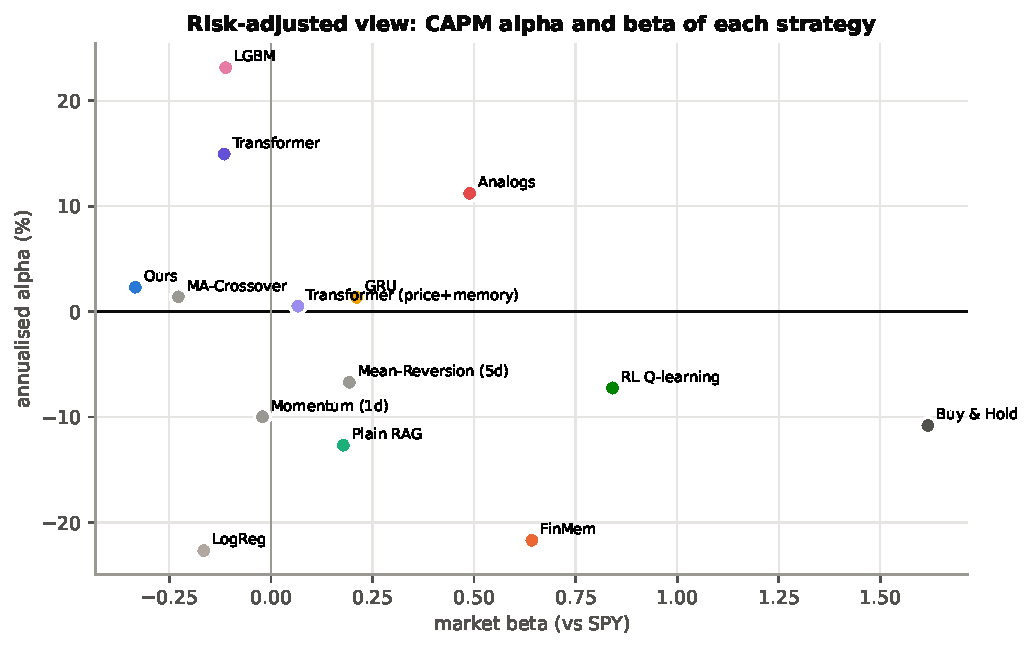
\includegraphics[width=0.85\textwidth]{fig27_capm_alpha_beta.pdf}
\caption{Market beta and annualised CAPM alpha of every strategy against the S\&P 500.}
\label{fig:capm}
\end{figure}

\subsection{Does Tesla drive the result?}
Tesla fell $5.3\%$ over the test window and was the stock on which our memory did worst (Sharpe $-1.39$). Table~\ref{tab:ext-robust} and Figure~\ref{fig:robust} recompute the portfolio without it. Our memory improves from $-0.20$ to $+0.23$ and FinMem from $-0.72$ to $-0.43$, but the ranking does not change: buy-and-hold ($0.67$), LightGBM ($0.92$) and the Transformer ($0.79$) remain ahead. Leaving out each stock in turn, our memory beats FinMem in 9 of 10 cases (the exception is leaving out COIN), and the Sharpe advantage ranges from $-0.34$ to $+1.11$ around the full-sample $+0.52$. The comparison between memories is therefore not an artefact of one stock, while the conclusion that news memory does not beat buy-and-hold also holds without Tesla. Choosing the end of the test period by waiting for any stock to recover would bias the evaluation and was deliberately avoided.

\begin{table}[H]
\centering
\small
\caption{Robustness to the stock set: Sharpe with all ten stocks, without Tesla, and on FinMem's five stocks.}
\label{tab:ext-robust}
\begin{tabular}{lrrr}
\toprule
Model & 10 stocks & without TSLA & FinMem's 5 \\
\midrule
Buy \& Hold & +0.61 & +0.67 & -0.34 \\
LGBM (price) & +1.15 & +0.92 & +0.74 \\
Ours & -0.20 & +0.23 & +0.28 \\
FinMem & -0.72 & -0.43 & -1.59 \\
Plain RAG & -0.65 & -0.10 & -1.59 \\
Transformer (price) & +0.95 & +0.79 & +0.77 \\
RL Q-learning & +0.39 & +0.59 & -0.77 \\
\bottomrule
\end{tabular}
\end{table}


\begin{figure}[H]
\centering
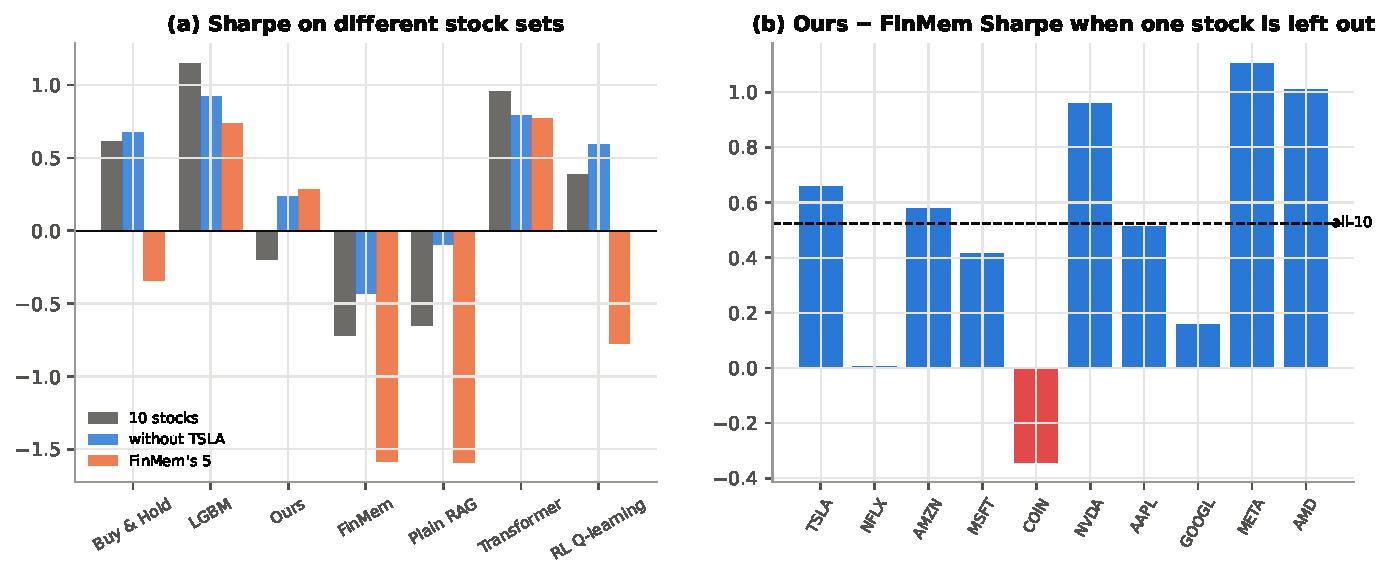
\includegraphics[width=\textwidth]{fig28_robustness.pdf}
\caption{Robustness: (a) Sharpe ratio on all ten stocks, without Tesla and on FinMem's five stocks; (b) Sharpe advantage of our memory over FinMem when one stock is left out (dashed line: all ten stocks).}
\label{fig:robust}
\end{figure}

\subsection{Market regimes}
Table~\ref{tab:ext-regimes} and Figure~\ref{fig:regimes} split the test days by whether the S\&P 500 rose (117 days) or fell (110 days). Buy-and-hold gains about 100 basis points on up days and loses about 95 on down days. Our memory and the Transformer behave in the opposite way, losing slightly on up days and gaining 16--19 basis points on down days, and LightGBM gains a little on both (6 and 11 basis points); FinMem and the Q-learning agent follow the market. Models that hedge market falls are attractive as diversifiers, but over a rising year they lag buy-and-hold.

\begin{table}[H]
\centering
\small
\caption{Average daily result (basis points) on days when the S\&P 500 rose versus fell.}
\label{tab:ext-regimes}
\begin{tabular}{lrr}
\toprule
Strategy & up days & down days \\
\midrule
Buy \& Hold & +100.2 & -94.6 \\
LGBM (price) & +6.2 & +11.0 \\
Ours & -17.2 & +15.9 \\
FinMem & +35.8 & -47.6 \\
Plain RAG & +8.5 & -17.1 \\
Transformer (price) & -8.0 & +19.3 \\
RL Q-learning & +53.8 & -52.3 \\
Pattern analogs (kNN) & +32.2 & -18.7 \\
\bottomrule
\end{tabular}
\end{table}


\begin{figure}[H]
\centering
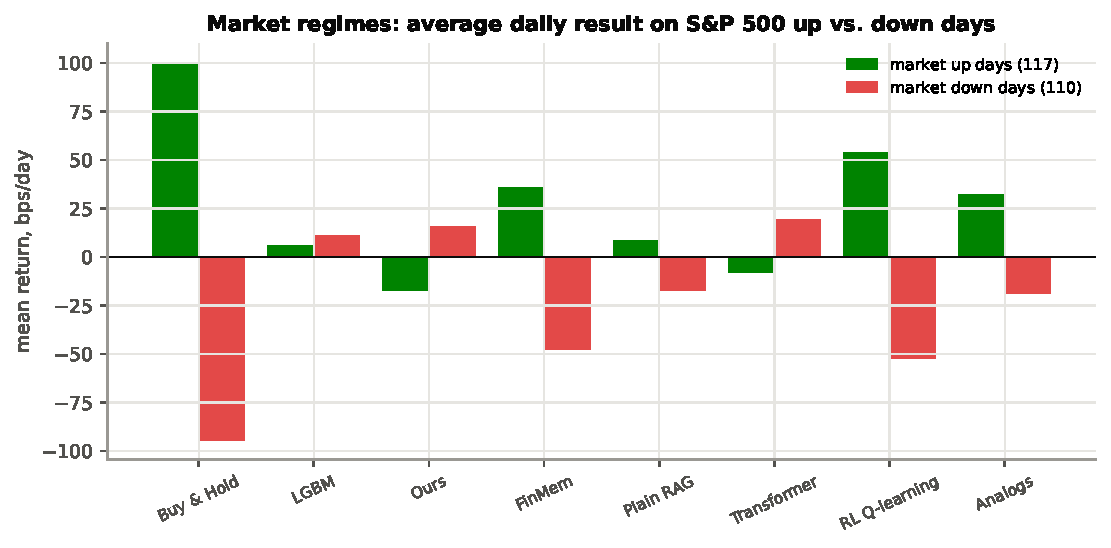
\includegraphics[width=\textwidth]{fig30_regimes.pdf}
\caption{Average daily result on days when the S\&P 500 rose versus fell.}
\label{fig:regimes}
\end{figure}
\begin{figure}[H]
\centering
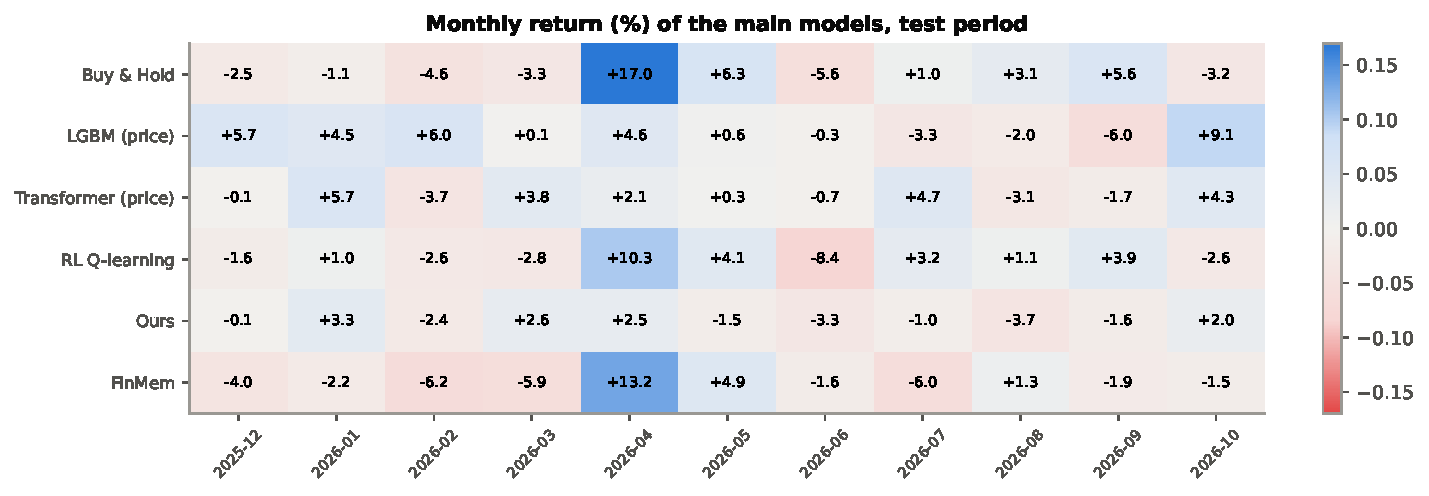
\includegraphics[width=\textwidth]{fig32_monthly_models.pdf}
\caption{Monthly returns of the main models in the test period.}
\label{fig:monthly-models}
\end{figure}

\subsection{Statistical power}
How much data would we need to prove that our memory beats FinMem? The daily difference between the two portfolios averages $\powerMean$ basis points with a standard deviation of $\powerSd$ basis points. With $\powerN$ days, a two-sided test at the 5\% level has 80\% power only for differences of at least $\powerMde$ basis points per day, seven times larger than the observed one. Detecting the observed edge with 80\% power would need about $\powerNeed$ trading days, roughly $\powerYears$ years (Figure~\ref{fig:power}). No realistic extension of the test period, and certainly not waiting a few weeks for a stock to recover, can turn this comparison into a significant result. The honest conclusion is that the memory comparison is \emph{directionally consistent} (positive in 9 of 10 leave-one-out cases, on FinMem's own stocks and with every LLM backbone) but \emph{statistically inconclusive}.

\begin{figure}[H]
\centering
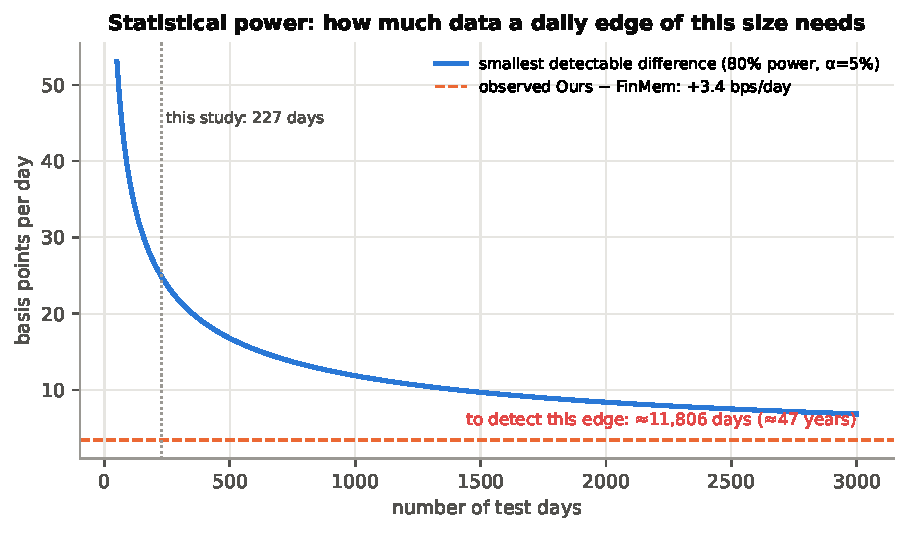
\includegraphics[width=0.85\textwidth]{fig29_power.pdf}
\caption{Smallest daily return difference detectable with 80\% power as a function of the number of test days, compared with the observed difference between our memory and FinMem.}
\label{fig:power}
\end{figure}

\subsection{Risk profile of the universe}
Table~\ref{tab:ext-stock-risk} and Figure~\ref{fig:market-risk} describe the stocks themselves. Annualised volatility ranges from 25\% (AAPL) to 69\% (COIN and AMD); COIN fell 64\% from its peak. The pairwise correlations are moderate (mostly 0.1--0.5), while the stocks' correlations with the S\&P 500 and Nasdaq-100 reach 0.6--0.7, so a large part of every stock's movement is common market risk. These numbers also explain why risk-parity weights favour AAPL and MSFT and give little to COIN and AMD.

\begin{table}[H]
\centering
\small
\caption{Risk profile of each stock over the full price history (Aug 2025 -- Oct 2026).}
\label{tab:ext-stock-risk}
\resizebox{\textwidth}{!}{%
\begin{tabular}{lrrrrrrr}
\toprule
Stock & Vol/yr & MDD & VaR$_{95}$ & CVaR$_{95}$ & $\beta$ & Skew & Ex.\ kurt. \\
\midrule
TSLA & 45\% & -39.1\% & 4.3\% & 5.9\% & 2.27 & -0.29 & 1.82 \\
NFLX & 35\% & -50.5\% & 3.4\% & 5.2\% & 0.29 & +0.17 & 6.95 \\
AMZN & 33\% & -21.7\% & 3.0\% & 4.0\% & 1.46 & +1.49 & 9.58 \\
MSFT & 30\% & -34.5\% & 2.7\% & 3.8\% & 0.99 & +1.35 & 15.55 \\
COIN & 69\% & -63.6\% & 6.5\% & 8.2\% & 2.93 & +0.53 & 1.11 \\
NVDA & 36\% & -20.2\% & 3.7\% & 4.5\% & 1.91 & +0.17 & 0.67 \\
AAPL & 25\% & -13.8\% & 2.0\% & 3.4\% & 0.69 & -0.24 & 3.06 \\
GOOGL & 31\% & -21.2\% & 2.5\% & 3.7\% & 1.38 & +0.77 & 3.78 \\
META & 40\% & -33.3\% & 3.5\% & 5.7\% & 1.48 & +0.21 & 4.39 \\
AMD & 69\% & -27.8\% & 5.9\% & 8.0\% & 3.13 & +0.73 & 4.00 \\
\bottomrule
\end{tabular}
}
\end{table}


\begin{figure}[H]
\centering
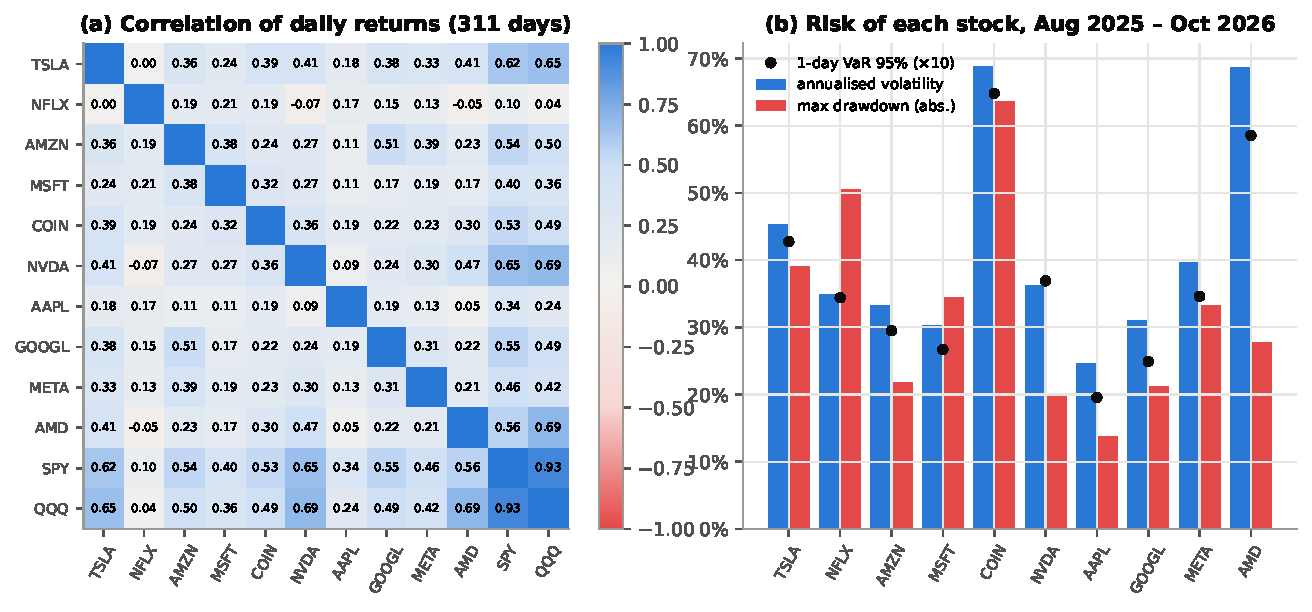
\includegraphics[width=\textwidth]{fig31_market_risk.pdf}
\caption{Market structure: (a) correlation of daily returns over the full history; (b) volatility, maximum drawdown and one-day 95\% value-at-risk of each stock.}
\label{fig:market-risk}
\end{figure}

\section{The Application}
\label{sec:app-results}
The application operationalises these findings. Because no single signal is reliable, its default recommendation is a conservative consensus: the memory action and the price-model vote must not disagree, the price model votes only when $|P(\text{up})-0.5|\ge 0.03$, episodic abstention forces Hold, and confidence is capped at 0.6. The LLM sees exactly the context used in the study and must cite memory IDs, which the interface highlights so that the user can verify the rationale. A refresh action downloads new news, prices and filings, annotates only the new items and replays the memory.

\paragraph{Safe autonomy.} The AI Autopilot (Figure~\ref{fig:ui-autopilot}) can run on a schedule during U.S.\ market hours, but every order passes the hard guardrail of Section~\ref{sec:autopilot-design}, and the default permission mode asks the user to approve each trade. In testing, the guardrail correctly sized orders by the tightest limit, blocked new buys after the daily-loss or drawdown limit while still allowing exits, refused stocks outside the allowed list, expired unanswered proposals and re-checked approvals; the emergency stop cancelled the queue and prevented the autopilot from being restarted until the user resumed trading. A safety gap of the earlier prototype was found and closed during this work: in Alpaca mode, agent orders used to bypass the position and loss limits because those were only implemented in the local simulator; all agent orders now pass the same guardrail regardless of the broker.
\paragraph{Insights for non-specialists.} The Insights page turns the analyses of this chapter into interactive tools for the selected stock: the budget split (Figure~\ref{fig:ui-split}), the pattern finder (Figure~\ref{fig:ui-pattern}), a Monte Carlo ``what-if'' that resamples historical days to show the distribution of future account values (Figure~\ref{fig:ui-whatif}), a risk report and a correlation matrix (Figure~\ref{fig:ui-risk}), and the algorithm board (Figures~\ref{fig:ui-algo}--\ref{fig:ui-rl}). The board answers the question users most often ask about an AI recommendation, ``how often has this been right?'': for each of 18 algorithms it shows today's call next to its out-of-sample hit rate, return, Sharpe ratio and full decision log, read directly from the study's results file.

\begin{figure}[!htbp]
\centering
\appshot{app_whatif_paper.png}
\caption{What-if: where the money is today (allocation and share of risk) and 2{,}000 simulated futures of the account value.}
\label{fig:ui-whatif}
\end{figure}
\begin{figure}[!htbp]
\centering
\appshot{app_risk_paper.png}
\caption{Risk tab for COIN: distribution of daily returns against a normal curve, value-at-risk and drawdown history.}
\label{fig:ui-risk}
\end{figure}
\begin{figure}[!htbp]
\centering
\appshot{app_algorithms_board_paper_1.png}
\caption{Algorithm board for NVDA: what each of 18 algorithms says today, with its out-of-sample record and a growth sparkline; the box names the experience data file.}
\label{fig:ui-algo}
\end{figure}
\begin{figure}[!htbp]
\ContinuedFloat
\centering
\appshot{app_algorithms_board_paper_2.png}
\caption[]{(continued)}
\end{figure}
\begin{figure}[!htbp]
\centering
\appshot{app_experience_paper.png}
\caption{Experience log of one algorithm: every decision, the position held, the next-day move and whether it was right.}
\label{fig:ui-experience}
\end{figure}
\begin{figure}[!htbp]
\centering
\appshot{app_rl_paper_1.png}
\caption{The Q-learning agent in the application: how it works in four steps, today's situation and Q-values, learning curve, test against buy-and-hold, learned Q-table and its most recent experiences.}
\label{fig:ui-rl}
\end{figure}
\begin{figure}[!htbp]
\ContinuedFloat
\centering
\appshot{app_rl_paper_2.png}
\caption[]{(continued)}
\end{figure}

\paragraph{Usability and quality.} The interface is available in English and Bangla (about 750 strings, checked automatically for completeness), in light and dark themes and on phones (Figure~\ref{fig:ui-mobile}). Figure~\ref{fig:ui-home-bn} shows the Home page of Figure~\ref{fig:ui-home} in Bangla: every label, explanation and status message is translated, while prices and percentages keep Latin digits so that numbers stay unambiguous. Testing in a headless browser also revealed and fixed several defects: the trade chart showed Tesla's prices for five of the ten stocks and drew synthetic candles (it now uses the real daily bars of each stock), two ``sell'' buttons called functions that did not exist, ``limit'' and ``stop'' order types were silently executed as market orders (they were removed), and two pages shared element identifiers so that one page's chart was drawn into another. API keys can be added from the interface and are verified with the provider before they are stored; the browser never receives a full key.

\begin{figure}[!htbp]
\centering
\appshot{app_home_bn_paper.png}
\caption{The Home page of Figure~\ref{fig:ui-home} in Bangla.}
\label{fig:ui-home-bn}
\end{figure}

\section{Summary}
We implemented and tested the full pipeline, five extension models and the application. Our memory is the strongest of the memory architectures under the primary protocol and on FinMem's own stocks, with lower drawdown, but the improvement is not statistically significant, the predictive content of news memory is close to zero, and buy-and-hold and a price-only model are better over this period. Results also depend strongly on the evaluation protocol and on $K$, which supports rigorous walk-forward evaluation for LLM trading agents. The extension experiments confirm these conclusions with other model families: a small Transformer on price features is competitive with buy-and-hold and LightGBM, adding news-memory features hurts it as it hurts LightGBM, a Q-learning agent mostly learns to stay invested, and an apparently strong chart-pattern result is fragile across settings. CAPM, leave-one-out and regime analyses show that the memory comparison is not driven by Tesla and that the gap to buy-and-hold is largely explained by market exposure, while a power analysis shows that about $\powerYears$ years of data would be needed to establish the observed edge statistically.

\chapter{Standards and Design Constraints}
\label{ch:sic}

This chapter lists the standards our design complies with, the constraints that shaped it, a cost analysis with an alternative budget, and the mapping of the project to complex engineering problem and activity attributes.

\section{Compliance with the Standards}

\subsection{Software Standards}
\begin{itemize}
  \item \textbf{Python PEP~8 / PEP~484}: code style and type hints throughout the package; alternatives (no style guide, or a different language) would reduce readability for future students.
  \item \textbf{ISO/IEC/IEEE 29119 (software testing)} principles: requirement-linked unit and integration tests (\testcount{} automated tests, run before each commit), including tests that encode the no-look-ahead requirement.
  \item \textbf{Semantic versioning and packaging (PEP~621)}: the project is an installable package with declared dependencies and console entry points.
  \item \textbf{Reproducible research practice}: versioned data, fixed random seeds, cached LLM responses keyed by prompt hash, and scripts that regenerate every table and figure. The alternative of reporting hand-copied numbers was rejected because it is error-prone.
\end{itemize}

\subsection{Hardware Standards}
The system runs on commodity x86-64 hardware and needs no GPU; inference uses CPU builds of PyTorch. This was preferred over GPU-dependent pipelines because it keeps the project reproducible on student laptops.

\subsection{Communication Standards}
\begin{itemize}
  \item \textbf{HTTP/1.1 over TLS (HTTPS)} and \textbf{REST with JSON (RFC~8259)} for all external APIs (Alpaca, SEC EDGAR, Groq, OpenRouter) and for the application's own API.
  \item \textbf{OpenAI-compatible chat-completions schema} for LLM providers, which lets the same client address several providers; provider-specific SDKs were avoided to keep backbones interchangeable.
  \item \textbf{SEC EDGAR fair-access policy}: requests identify the client in the User-Agent header and respect rate limits.
  \item \textbf{ISO~8601} dates and \textbf{IANA time zones} (America/New\_York) for point-in-time alignment.
  \item \textbf{Same-origin policy and CORS (Fetch standard)}: endpoints that read or change API keys and trading controls check the request's \texttt{Origin} and \texttt{Host} headers and only accept the local machine.
\end{itemize}

\subsection{Usability and Accessibility Standards}
\begin{itemize}
  \item \textbf{WCAG~2.1 principles}: colour is never the only carrier of meaning (signs, labels and icons accompany green/red), interactive elements have accessible names, focus is visible, and both a light and a dark theme are offered.
  \item \textbf{Unicode and localisation}: the whole interface is available in English and Bangla (UTF-8, Bengali script with a Bengali web font); numbers keep Latin digits so that prices are unambiguous.
  \item \textbf{Responsive design}: the layout adapts from desktop to phone width (sidebar becomes a bottom navigation bar).
\end{itemize}

\section{Design Constraints}
\subsection{Economic Constraint}
The project had no budget for paid data or inference. We therefore used Alpaca's free news and market data, SEC EDGAR, open encoders (FinBERT, MiniLM) and free LLM tiers. The free tiers limit the LLM experiment (on Groq, 8{,}000 tokens per minute and 200{,}000 tokens per day per model and account; on OpenRouter, 50 free-model requests per day per account), which is why it covers five stocks and 50 sessions with a single trial per model and three backbones.

\subsection{Environmental Constraint}
Running small open encoders on a CPU once and caching their outputs uses far less energy than sending every article to a large hosted LLM. LLM calls are cached so that re-running analyses consumes no additional inference.

\subsection{Ethical Constraint}
The system is a research and decision-support tool, not financial advice. It reports negative and non-significant results explicitly, separates post-hoc variants from pre-specified ones, and the application displays the study's limitations next to its recommendations. News content is used only as headline-level text for research; full articles are not redistributed.

\subsection{Health and Safety Constraint}
Automated trading can cause financial harm. Paper trading is the default; live trading requires both a command-line flag and an environment confirmation. When the agent is allowed to act autonomously, every order passes one server-side guardrail with user-defined hard limits (budget, cash reserve, per-stock and per-order caps, daily-loss and drawdown limits, trades per day); the default permission mode requires the user's approval for each trade; switching to fully automatic mode shows an explicit warning that our research found the signals weak; and an emergency stop pauses the agent, cancels pending orders and can close all positions.

\subsection{Social Constraint}
Over-confident trading tools can encourage retail investors to take excessive risk. The interface therefore shows confidence capped at 60\%, highlights disagreement between models, links each decision to the evidence it relies on, shows every algorithm's out-of-sample track record next to its current advice, and explains metrics in plain language in English and Bangla so that users who are not finance specialists can judge the risk.

\subsection{Political Constraint}
Data providers' terms of service and securities regulation constrain use. We use data only within the providers' terms, do not execute live trades by default and make no claims of guaranteed returns.

\subsection{Sustainability}
The modular design (data, memory, policies, evaluation, application) lets future students replace components, add tickers or data sources, and re-run the full study with a few commands. Incremental refresh keeps the dataset current without re-downloading or re-annotating history.

\section{Cost Analysis}
\begin{table}[H]
\centering
\caption{Budget used and an alternative (paid) budget for a comparable study.}
\label{tab:cost}
\begin{tabular}{lrr}
\hline
Item & Used (USD) & Alternative (USD) \\
\hline
News and market data (Alpaca free / paid SIP) & 0 & 99 per month \\
SEC filings (EDGAR) & 0 & 0 \\
Annotation (FinBERT, MiniLM on CPU / GPT-4-class API) & 0 & $\approx$ 50--150 \\
LLM decisions (free tiers / paid API, 3 models) & 0 & $\approx$ 20--60 \\
Cloud compute (laptop / small cloud VM) & 0 & $\approx$ 30 per month \\
\hline
Total for the study & 0 & $\approx$ 200--350 \\
\hline
\end{tabular}
\end{table}
The alternative budget would remove the free-tier limits (more LLM trials, larger universes, full filing text) and is the recommended path for extending the work. A possible revenue model for the application is a subscription for analysts who want inspectable, evidence-linked news monitoring, with live-trading integration offered only to licensed users.

\section{Complex Engineering Problem}
\subsection{Complex Problem Solving}
\begin{table}[H]
\centering
\caption{Mapping with complex problem solving.}
\label{tab:p_solve}
\small
\setlength{\tabcolsep}{4pt}
\begin{tabular}{|*{7}{C{0.105\textwidth}|}}
\hline
P1 & P2 & P3 & P4 & P5 & P6 & P7\\
Depth of Knowledge & Range of Conflicting Require\-ments & Depth of Analysis & Familiarity of Issues & Extent of Applicable Codes & Extent of Stakeholder Involvement & Inter\-dependence\\
\hline
$\surd$ & $\surd$ & $\surd$ & $\surd$ & & & $\surd$\\
\hline
\end{tabular}
\end{table}
\paragraph{P1 Depth of knowledge.} The project requires knowledge of NLP (transformers, embeddings), information retrieval, LLM agents, financial markets and microstructure (point-in-time data, costs), machine learning and non-parametric statistics. Table~\ref{tab:k_profile} maps it to the knowledge profiles.
\begin{table}[H]
\centering
\caption{Mapping of P1 with the knowledge profiles.}
\label{tab:k_profile}
\small
\begin{tabular}{|p{0.08\textwidth}|p{0.3\textwidth}|p{0.52\textwidth}|}
\hline
Profile & Attribute & Rationale in this project \\
\hline
K2 & Mathematics, statistics and computing & Decay and scoring functions, Beta--Bernoulli credibility, Wilcoxon, Holm, Diebold--Mariano, block bootstrap, CAPM regression and power analysis \\
K3 & Engineering fundamentals & Data structures for the memory store, algorithm design of the day-major replay, software architecture of package and application \\
K4 & Specialist knowledge & Transformer encoders (FinBERT, MiniLM), retrieval-augmented LLM agents, GRU/Transformer forecasting, Q-learning, financial markets \\
K5 & Engineering design & Design of the seven memory components, the evaluation protocols and the safe-autonomy guardrail \\
K6 & Engineering practice & Automated testing, reproducible pipelines, REST APIs of data, LLM and broker providers, credential handling \\
K7 & Engineering in society & Financial risk to users, honest reporting of negative results, paper trading by default, human approval \\
K8 & Research literature & Re-evaluation of FinMem and related LLM-agent, memory and back-testing literature \\
\hline
\end{tabular}
\end{table}
\paragraph{P2 Conflicting requirements.} Realism versus cost (free tiers), responsiveness versus rigour (incremental refresh versus full replay), and autonomy versus safety (agent decisions versus human approval).
\paragraph{P3 Depth of analysis.} No closed-form solution exists; designs were compared through controlled ablations, two protocols, sensitivity analyses and significance tests.
\paragraph{P4 Familiarity of issues.} Look-ahead bias, selection bias and regime dependence are subtle, uncommon issues that invalidate many published back-tests and had to be identified and controlled.
\paragraph{P7 Inter\-dependence.} Data alignment, annotation, memory, policies, evaluation and the application depend on one another; a timing error in one stage silently corrupts all later results.

\subsection{Engineering Activities}
\begin{table}[H]
\centering
\caption{Mapping with complex engineering activities.}
\label{tab:e_act}
\small
\begin{tabular}{|*{5}{C{0.16\textwidth}|}}
\hline
A1 & A2 & A3 & A4 & A5\\
Range of resources & Level of Interaction & Innovation & Consequences for society and environment & Familiarity\\
\hline
$\surd$ & $\surd$ & $\surd$ & $\surd$ & \\
\hline
\end{tabular}
\end{table}
\paragraph{A1 Range of resources.} Four external services, pretrained models, open-source libraries and a team of five.
\paragraph{A2 Level of interaction.} The system interacts with data providers, LLM providers, a broker and the user, and the user remains in the loop for every order.
\paragraph{A3 Innovation.} Seven new memory components and a stricter evaluation protocol for LLM trading agents.
\paragraph{A4 Consequences.} Automated trading advice can affect users' finances; safety guards, transparency and honest reporting address this.

\section{Summary}
The design follows software, communication and data-access standards, is shaped by economic, ethical and safety constraints, was completed at zero monetary cost, and addresses a complex engineering problem across several knowledge areas.

\chapter{Conclusion}
\label{ch:concl}

This chapter summarises the work, discusses its limitations and outlines future work.

\section{Summary}
We designed a self-correcting agent memory for LLM trading agents and evaluated it on a point-in-time dataset of 23{,}247 news articles, 93 SEC filings and daily prices for ten stocks over September 2025 -- October 2026, against a faithful re-implementation of FinMem and other baselines. On top of a layered long-term memory, it adds hierarchical online source credibility, duplicate consolidation, contradiction retirement, a situational query, data-driven importance, a co-mention peer graph and outcome-aware episodic recall. Under a rolling walk-forward evaluation with transaction costs, our memory was the best of the evaluated memory architectures (Sharpe $-0.20$ versus $-0.72$ for FinMem, maximum drawdown $-15.2\%$ versus $-19.7\%$) and turned FinMem's own five stocks from a $-28.6\%$ loss into a $+3.5\%$ gain. With three LLM backbones reading the retrieved context, our memory also beat FinMem's context with every backbone and roughly halved the drawdown. These improvements are not statistically significant; the next-day predictive content of every news-memory signal was close to zero; and buy-and-hold and a price-only LightGBM model performed better in this period. Results also changed sign between a fixed split and the rolling protocol and varied strongly with the number of retrieved memories. Five additional model families evaluated on the same protocol support the same picture: a small price-only Transformer was competitive with buy-and-hold (Sharpe $0.95$, smallest drawdown), adding our news-memory features lowered its Sharpe to $0.09$ just as they lowered LightGBM's, a Q-learning agent mostly followed the market, and an apparently strong chart-pattern result was fragile across settings. Robustness analyses showed that our memory beats FinMem in 9 of 10 leave-one-stock-out comparisons, that the gap to buy-and-hold is largely due to a negative market beta in a rising year, and that about 47 years of daily data would be needed to establish the observed edge over FinMem at conventional significance. Our main conclusions are therefore that (i) agent memory design measurably changes the retrieved context (fresher, credibility-weighted, with duplicates merged and contradicted facts retired) and the risk profile of the agent, and verifying memories against source reliability and past outcomes works above all as a risk control; (ii) LLM trading agents should be evaluated walk-forward, with costs and significance tests, before any claim of outperformance; and (iii) under such an evaluation, the gains reported for existing layered memory do not transfer to recent data. We packaged the agent in a bilingual application for non-specialist users that exposes its evidence and every algorithm's out-of-sample record, advises how to split a budget, and lets the agent act autonomously only inside user-defined guardrails, with a human-approval mode as the default.

\section{Limitation}
\begin{itemize}
  \item \textbf{Period and universe}: about one year and ten liquid large caps; results may differ for small caps, other markets or longer horizons.
  \item \textbf{Signals}: headline-level FinBERT polarity and numeric XBRL summaries replace FinMem's GPT-generated summaries of full articles and filings; richer text could carry more information.
  \item \textbf{Decision horizon}: only next-day close-to-close trading was evaluated; news may matter more at intraday or multi-week horizons.
  \item \textbf{LLM experiment}: free-tier limits restricted it to three backbones, five stocks, 50 sessions and one trial per model at temperature 0; the backbones agree on only about a quarter of the decisions, so more trials and models are needed.
  \item \textbf{Statistical power}: 227 sessions are too few to detect small daily differences; non-significance does not prove equality.
  \item \textbf{Post-hoc analysis}: one variant (signed credibility) and two combinations (risk overlay, model vote) were designed after seeing test results; they are reported separately and excluded from the main conclusions.
  \item \textbf{Model capacity}: the GRU and Transformer are deliberately small and the Q-learning agent uses a coarse 36-state description of the market; larger models and richer states need far more data than one year of daily bars.
  \item \textbf{Multiple comparisons in the extensions}: twelve models were compared; the best one (pattern analogues) is exactly the kind of winner that selection inflates, which is why its sensitivity grid is reported.
  \item \textbf{Application}: the autopilot was tested on a paper account and with unit tests; it has not been operated over a long live period, and exchange holidays are not modelled in its market-hours check.
\end{itemize}

\section{Future Work}
\begin{itemize}
  \item Extend the data to several years and a broader universe, and evaluate multi-day and intraday horizons where news effects may be stronger.
  \item Summarise full articles and filing text with an LLM to enrich memory, and measure whether richer memory changes the predictive content.
  \item Use the memory as a risk overlay (position sizing, abstention) on top of a price model rather than as a stand-alone signal, as suggested by the drawdown effect of N1 and N7 and by the exploratory overlay that cut LightGBM's drawdown from $-17.2\%$ to $-11.6\%$; this must be tested on new data because it was defined after the results were known.
  \item Pre-register an extension of the test window with a fixed end date and evaluate the frozen models on it, and pool evidence across more stocks and markets to approach the sample sizes the power analysis calls for.
  \item Replace the tabular Q-learning agent with deep RL (e.g.\ PPO) on richer states once several years of data are available, and evaluate pre-trained time-series Transformers.
  \item Run multi-trial LLM experiments with paid inference and compare reasoning and non-reasoning models.
  \item Add live forward testing on the paper account to complement back-tests.
\end{itemize}



\bibliographystyle{unsrt}
\bibliography{fydp}
\addcontentsline{toc}{chapter}{References}

\clearpage
\appendix
\chapter{Reproducing the Results}
\label{app:repro}

All numbers, tables and figures in this report are produced by scripts from versioned data. On a laptop with Python~3.13:

\begin{verbatim}
python -m venv .venv && .venv/bin/pip install -e .[all] -r requirements.txt
# 1. dataset (needs free Alpaca keys; SEC EDGAR needs none)
.venv/bin/python scripts/build_dataset.py
# 2. main study: memory replay, both protocols, tables, figures 1-20
.venv/bin/python scripts/run_study.py --figures
# 3. LLM backbone experiment (needs free Groq keys)
.venv/bin/python scripts/run_llm_study.py
# 4. extension models: GRU, Transformer, Q-learning, analogues
.venv/bin/python scripts/run_extensions.py
# 5. figures 21-32 and LaTeX tables
.venv/bin/python scripts/make_extension_figures.py
.venv/bin/python scripts/export_latex_tables.py
.venv/bin/python scripts/export_extension_tables.py
.venv/bin/python scripts/crop_paper_screens.py   # screenshots sized for A4
# 6. tests and application
.venv/bin/python -m pytest -q
./run_dashboard.sh            # http://localhost:8050
\end{verbatim}

\chapter{Hyperparameters}
\label{app:hyper}

\begin{table}[H]
\centering
\small
\caption{Settings of every model. All were fixed before the test period was evaluated, except the two exploratory combinations.}
\label{tab:hyper}
\begin{tabular}{p{0.24\textwidth}p{0.68\textwidth}}
\toprule
Component & Settings \\
\midrule
FinMem & $Q=14/90/365$ days; $\alpha=0.9/0.967/0.988$; importance $v\in\{40,60,80\}$; purge at recency $<0.05$ or importance $<5$; access bonus $+5$; top-$K=5$ per layer \\
Ours (N1--N7) & FinMem core; hierarchical Beta--Bernoulli credibility (author $\rightarrow$ category $\rightarrow$ global, prior strength 8); duplicates: cosine $\ge0.88$ with the same polarity sign; contradiction: cosine $\ge0.72$, opposite polarity, $|s|\ge0.3$; 3 peers; episodic recall over the 10 nearest past contexts, at least 5 required \\
Threshold rule & $\theta\in\{0,0.05,0.1,0.15,0.2,0.3,0.4\}$, re-selected monthly on the previous 42 sessions \\
LightGBM & 200 trees, learning rate 0.03, 15 leaves, min.\ 40 samples per leaf, subsample 0.8, column sample 0.8, $\lambda=1$; 3 seeds \\
Logistic regression & standardised features, $C=0.5$ \\
GRU & 20-day window, 9 price features, hidden size 32, ticker embedding 4, dropout 0.2 \\
Transformer & 20-day window, $d=32$, 2 layers, 2 heads, feed-forward 64, dropout 0.1, learned positions, ticker embedding \\
Deep training & BCE loss, AdamW ($10^{-3}$, weight decay $10^{-3}$), batch 64, clip 1.0, $\le40$ epochs, early stopping patience 6 on the last 15\% of training rows, 3 seeds, monthly refit \\
Q-learning & 36 states, actions Flat/Long, $\alpha=0.1$, $\gamma=0.9$, 30 pre-training passes, $\varepsilon$ from 1 to 0.05, online updates in the test window, cost 5\,bps per switch \\
Pattern analogues & window 20 days, horizon 10 days, $k=8$, same-stock search, threshold 1\%, $P(\text{up})$ bounds 0.55/0.45 \\
Decision margin (ML/DL) & long if $P(\text{up})>0.52$, short if $<0.48$, otherwise keep \\
Costs & 5 basis points per unit of position change \\
Allocation back-test & 120-day estimation window, rebalance every 21 days, 20\% cash reserve, 25\% cap per stock \\
\bottomrule
\end{tabular}
\end{table}

\chapter{Application Programming Interface}
\label{app:api}

\begin{table}[H]
\centering
\small
\caption{Main HTTP endpoints of the application (JSON over HTTP on localhost).}
\label{tab:api}
\begin{tabular}{p{0.38\textwidth}p{0.55\textwidth}}
\toprule
Endpoint & Purpose \\
\midrule
\texttt{GET /api/portfolio} & account value, cash, positions, risk, orders \\
\texttt{GET /api/market\_data?ticker=} & daily OHLCV with indicators, live quote for today \\
\texttt{GET /api/agent/brief?ticker=} & retrieved memories, signals of the three memories, consensus \\
\texttt{POST /api/agent/llm} & LLM decision with the study prompt \\
\texttt{GET /api/agent/scan} & ten-stock scanner \\
\texttt{GET /api/research} & study results for the Research Lab \\
\texttt{GET /api/analytics/allocation} & budget split, rebalancing amounts, walk-forward comparison \\
\texttt{GET /api/analytics/analogs}, \texttt{/backtest}, \texttt{/sweep} & chart-pattern analogues and their evaluation \\
\texttt{GET /api/analytics/risk}, \texttt{/correlation}, \texttt{/portfolio} & risk report, correlation matrix, Monte Carlo equity distribution \\
\texttt{GET /api/analytics/algorithms}, \texttt{/experience}, \texttt{/rl} & algorithm board, decision log, Q-learning agent \\
\texttt{GET /api/autopilot/status} & limits, configuration, approval queue, activity log \\
\texttt{POST /api/autopilot/config} & save budget, limits and autopilot settings \\
\texttt{POST /api/autopilot/run\_once}, \texttt{/resolve}, \texttt{/kill}, \texttt{/resume}, \texttt{/rebalance} & run a check, approve/reject, emergency stop, resume, queue a rebalance \\
\texttt{GET /api/credentials}, \texttt{POST /api/credentials/save|test|remove} & key status (masked), verify and store, test, remove \\
\bottomrule
\end{tabular}
\end{table}

\chapter{User Guide (English and Bangla)}
\label{app:guide}

\begin{enumerate}
  \item \textbf{Connect accounts} (Settings $\rightarrow$ Connections): paste the Alpaca \emph{paper} key and secret and at least one Groq or OpenRouter key, then press \emph{Save \& test}. Only keys that the provider accepts are saved.
  \item \textbf{Set the budget} (Settings $\rightarrow$ Budget \& limits): total budget, cash to keep, the most that may go into one stock or one order, the daily-loss and drawdown limits and the stocks the AI may buy. A sentence under the form explains the limits in plain words.
  \item \textbf{Choose a stock} with the picker at the top; every page follows it.
  \item \textbf{Look before acting}: the Home page shows the AI's view in plain words, the Trade page the chart signals, the Insights pages the budget split, similar past charts, possible futures, risk, correlation and what every algorithm says with its track record.
  \item \textbf{Let the AI work}: on the AI Autopilot page choose how much freedom it gets (start with \emph{Ask me first}), how it decides and how often it checks, then start it. Approve or reject its proposals in the queue; the emergency stop halts everything.
  \item \textbf{Language and theme}: switch between English and Bangla and between light and dark mode in the top bar.
\end{enumerate}

\begin{figure}[H]
\centering
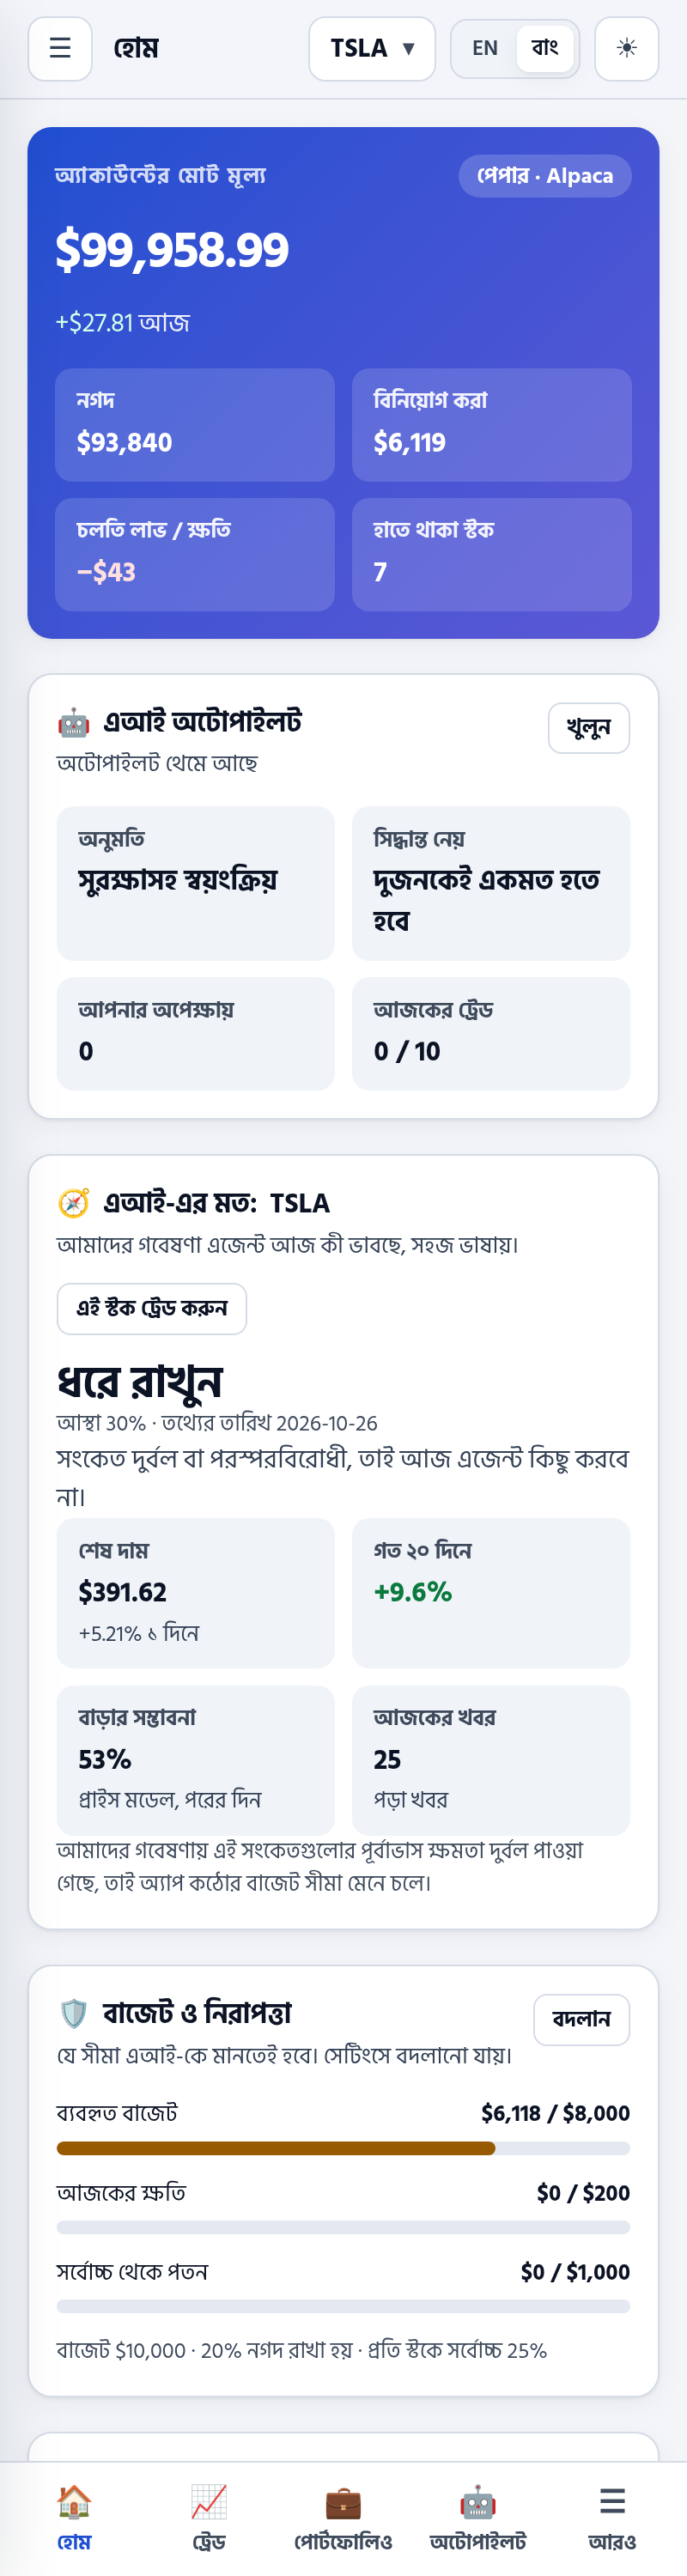
\includegraphics[height=0.8\textheight]{app_mobile_home_bn.png}
\hspace{0.03\textwidth}
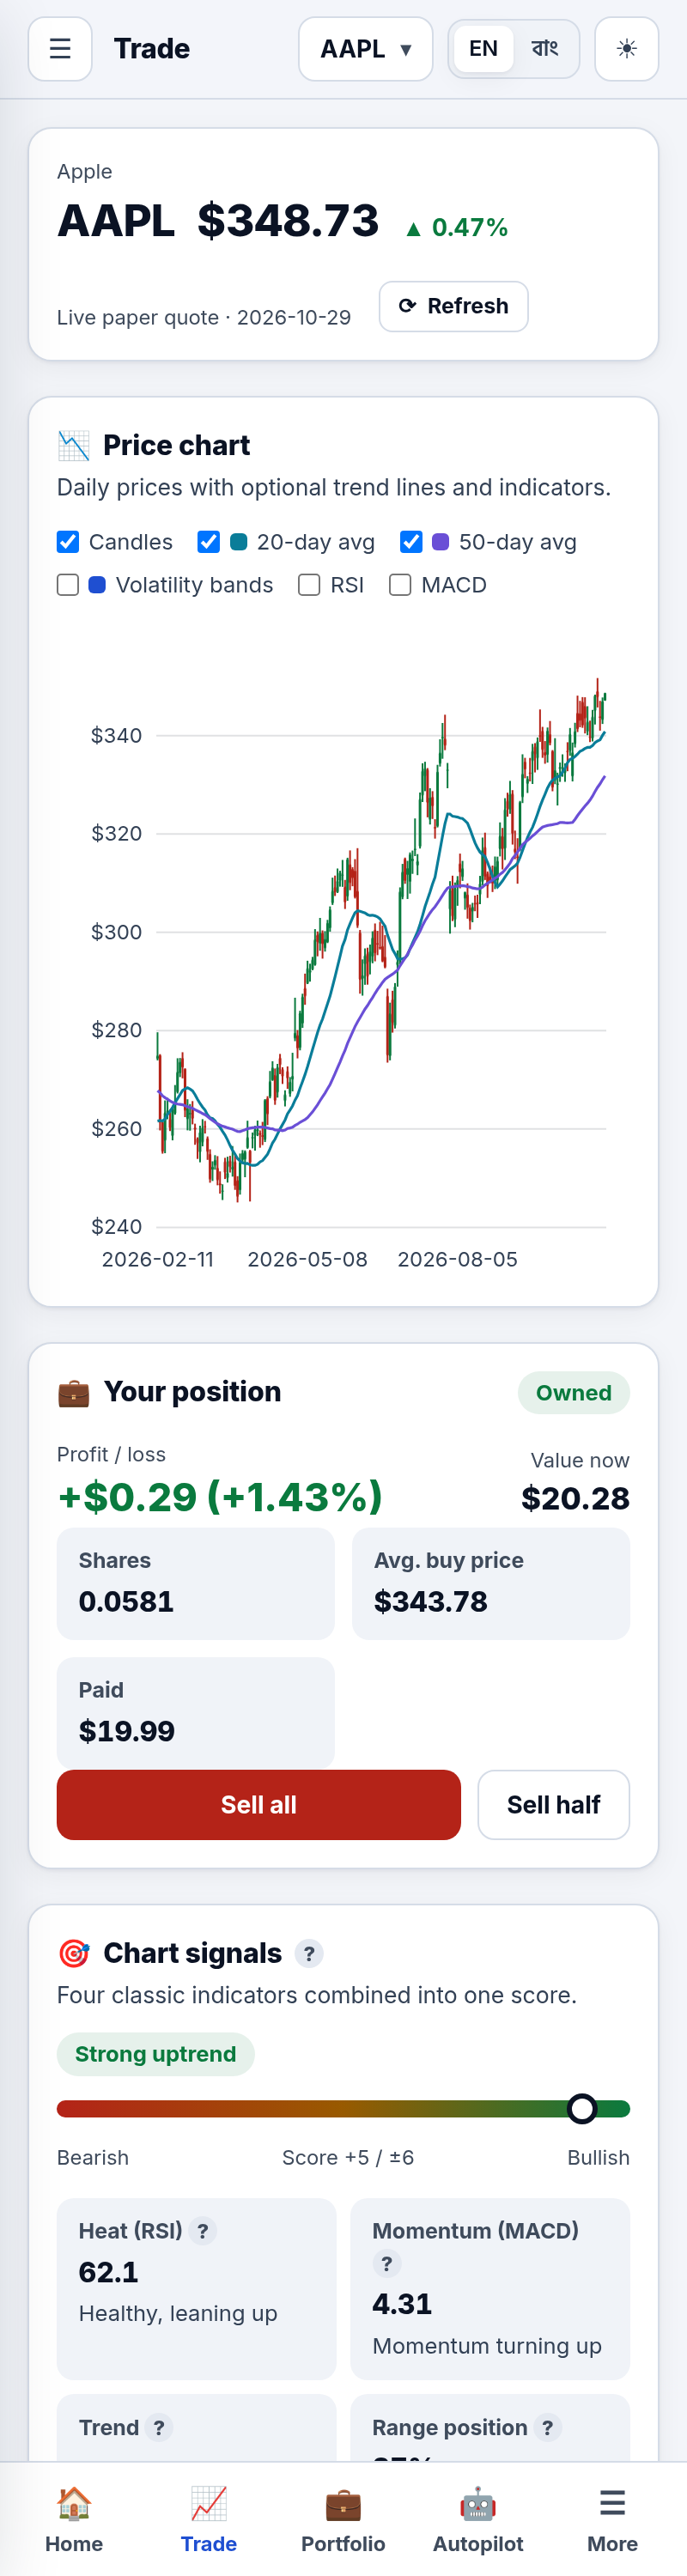
\includegraphics[height=0.8\textheight]{app_mobile_trade.png}
\caption{The application on a phone: Home in Bangla (left) and Trade in English (right).}
\label{fig:ui-mobile}
\end{figure}


%\phantomsection

%\addcontentsline{toc}{chapter}{Appendices}
%\chapter{Amino Acids\label{appAmino}}
%\begin{figure}[h]
%\begin{center}
%\includegraphics[width=1\textwidth]{./images/background/aminoacids}
%\end{center}
%\caption{Twenty different amino acids, their structures and chemical properties.\index{Amino Acid!chemical properties}\cite{Lehninger2012}.}
%\end{figure}
%\clearpage
%\thispagestyle{empty}
%\mbox{}

%\clearpage
%\phantomsection
%\addcontentsline{toc}{chapter}{Index}
%\printindex

\end{document}
